\chapter{Range-clone}
\label{chap:clone}

This chapter describes how to implement another type of namespace operations,
the file or directory clone, in a full-path-indexed file system.
File or directory clones are useful in many cases.
For example,
many people build versioning file systems~\citep{efs, cvfs, versionfs}
which constantly make read-only clones of files and directories.
Therefore, a user can get an old version of a file or directory after committing
unwanted changes to the file or directory.
Also, container applications usually clone the image file
before booting the container.

Similar to file or directory renames,
we implement file or directory clones with the range-clone operation on \bets.
Unlike a range-rename operation, which completes all its work at once,
a range-clone operation injects a new type of message, the \goto message,
into the root node of the \bet.
The \bet then flushes \goto messages with other messages in batches, gradually
finishing the range-clone work.
Therefore,
the range-clone operation fits into the write-optimized framework of \bets,
and the I/O cost of a range-clone operation is amortized with other operations.

Section~\ref{sec:rc:int} describes the range-clone interface and how to implement
file or directory renames and clones in full-path-indexed \betrfs by calling the
range-clone operation.
Section~\ref{sec:rc:rc} discusses how to implement the range-clone operation.
In particular, we first describe an implementation of the range-clone operation
with techniques introduced by the range-rename operation,
finishing all work on the critical path.
Then, we introduce the \goto message that delays most of the range-clone work
to the flushing process in the data structure.
Finally, Section~\ref{sec:rc:impl} explains some implementation details in the
range-clone operation.

\section{The range-clone interface}
\label{sec:rc:int}

Range-clone is defined as range-clone(\spre, \dpre).
Range-clone(\spre, \dpre) does the following things atomically:
\begin{itemize}
\item the range-clone operation deletes all destination key/value pairs from
    the key/value store;
\item then, for each source key/value pair $(k,v)$ in the key/value store,
    the range-clone operation creates a key/value pair $(k',v)$ to the
    key/value store, where $k$ is the concatenation of \spre and some suffix
    $s$ and $k'$ is the concatenation of \dpre and the same suffix $s$;
\end{itemize}
Therefore, range-clone(\spre, \dpre) is equivalent to range-rename(\spre, \dpre)
without deleting source key/value pairs.

\begin{table}[t]
    \centering
    \begin{tabular}{c | l}
        \hline
        Type of File System Operation & Key/Value Store Operations \\
        \hline
        \hline
        File Rename & transaction\_begin(); \\
                    & \mdb$\rightarrow$put(\textit{dst}); \\
                    & \mdb$\rightarrow$del(\textit{src}); \\
                    & \ddb$\rightarrow$range-clone(\textit{src}, \textit{dst}); \\
                    & \ddb$\rightarrow$range-delete(\textit{src}) \\
                    & transaction\_end(); \\
        \hline
        Directory Rename & transaction\_begin(); \\
                         & \mdb$\rightarrow$put(\textit{dst}); \\
                         & \mdb$\rightarrow$del(\textit{src}); \\
                         & \mdb$\rightarrow$range-clone(\textit{src/}, \textit{dst/}); \\
                         & \mdb$\rightarrow$range-delete(\textit{src/}); \\
                         & \ddb$\rightarrow$range-clone(\textit{src/}, \textit{dst/}); \\
                         & \ddb$\rightarrow$range-delete(\textit{src/}); \\
                         & transaction\_end(); \\
        \hline
        File Clone  & transaction\_begin(); \\
                    & \mdb$\rightarrow$put(\textit{dst}); \\
                    & \ddb$\rightarrow$range-clone(\textit{src}, \textit{dst}); \\
                    & transaction\_end(); \\
        \hline
        Directory Clone  & transaction\_begin(); \\
                         & \mdb$\rightarrow$put(\textit{dst}); \\
                         & \mdb$\rightarrow$range-clone(\textit{src/}, \textit{dst/}); \\
                         & \ddb$\rightarrow$range-clone(\textit{src/}, \textit{dst/}); \\
                         & transaction\_end(); \\
        \hline
    \end{tabular}
    \caption[Full-path-indexed \betrfs implements file system renames and clones with range-clone]{\label{tab:fsrc}
        Full-path-indexed \betrfs renames or clones \textit{src} to \textit{dst} by
        invoking range-clone and other operations on \bets.}
\end{table}

Table~\ref{tab:fsrc} summarizes how \betrfs implements file or
directory renames and clones by invoking the range-clone operation.
Because a range-clone operation is the same as a range-rename operation without
deleting the source key/value pairs,
\betrfs can complete a range-rename operation with a range-clone operation and
a range-delete operation (described in Section~\ref{sec:bg:fpi})
that deletes all source key/value pairs.
Therefore, \betrfs implements file or directory renames
by replacing the range-rename operation in Table~\ref{tab:fsrr} with
a range-clone operation and a range-delete operation.
And if \betrfs calls the range-clone operation without the range-delete
operation,
the source key/value pairs of metadata and data stay in the key/value store.
In such a scenario, the file system completes file or directory clones if it
doesn't delete the metadata for the source file or directory
(in rename, this delete is not covered in the range-rename operation).

Also, \betrfs puts all operations in a file system rename in a transaction
so that all changes are committed atomically.

\section{The range-clone operation}
\label{sec:rc:rc}

This section shows the implementation of the range-clone operation.

Section~\ref{sec:rc:crit} shows all the changes needed if we perform all
range-clone work on the critical path.
In particular, we show that the range-clone operation can be implemented
by modifying the range-rename operation.
This implementation shows all the work in the range-clone operation and
helps the understanding of the write-optimized implementation described in
later sections.
Then, Section~\ref{sec:rc:goto} introduces \goto messages.
The range-rename operation can return to the application immediately
after injecting a \goto message into the root node,
without slicing out the subtrees.
Finally, Section~\ref{sec:rc:flush} shows how \goto messages are flushed in
the data structure, gradually finishing the range-clone work.

\subsection{Range-clone, on the critical path}
\label{sec:rc:crit}

\begin{figure}
    \begin{subfigure}{\textwidth}
        \centering
        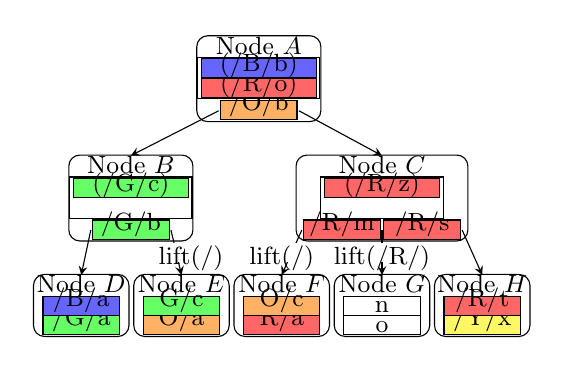
\begin{tikzpicture}
    \node[anchor=south, rectangle, rounded corners, minimum width=.1\textwidth, minimum height=.065\textwidth, draw=black] at (.0\textwidth, 0) {};
    \node[anchor=south, font=\small] at (.0\textwidth, .036\textwidth) {Node $F$};
    \node[anchor=south, rectangle, minimum width=.08\textwidth, minimum height=.02\textwidth, draw=black, fill={red!60}] at (.0\textwidth, .002\textwidth) {};
    \node[anchor=south, font=\small] at (.0\textwidth, -0.005\textwidth) {R/a};
    \node[anchor=south, rectangle, minimum width=.08\textwidth, minimum height=.02\textwidth, draw=black, fill={orange!60}] at (.0\textwidth, .022\textwidth) {};
    \node[anchor=south, font=\small] at (.0\textwidth, .015\textwidth) {O/c};

    \node[anchor=south, rectangle, rounded corners, minimum width=.1\textwidth, minimum height=.065\textwidth, draw=black] at (.105\textwidth, 0) {};
    \node[anchor=south, font=\small] at (.105\textwidth, .036\textwidth) {Node $G$};
    \node[anchor=south, rectangle, minimum width=.08\textwidth, minimum height=.02\textwidth, draw=black] at (.105\textwidth, .002\textwidth) {};
    \node[anchor=south, font=\small] at (.105\textwidth, -0.005\textwidth) {o};
    \node[anchor=south, rectangle, minimum width=.08\textwidth, minimum height=.02\textwidth, draw=black] at (.105\textwidth, .022\textwidth) {};
    \node[anchor=south, font=\small] at (.105\textwidth, .015\textwidth) {n};

    \node[anchor=south, rectangle, rounded corners, minimum width=.1\textwidth, minimum height=.065\textwidth, draw=black] at (.21\textwidth, 0) {};
    \node[anchor=south, font=\small] at (.21\textwidth, .036\textwidth) {Node $H$};
    \node[anchor=south, rectangle, minimum width=.08\textwidth, minimum height=.02\textwidth, draw=black, fill={yellow!60}] at (.21\textwidth, .002\textwidth) {};
    \node[anchor=south, font=\small] at (.21\textwidth, -0.005\textwidth) {/Y/x};
    \node[anchor=south, rectangle, minimum width=.08\textwidth, minimum height=.02\textwidth, draw=black, fill={red!60}] at (.21\textwidth, .022\textwidth) {};
    \node[anchor=south, font=\small] at (.21\textwidth, .015\textwidth) {/R/t};

    \node[anchor=south, rectangle, rounded corners, minimum width=.1\textwidth, minimum height=.065\textwidth, draw=black] at (-.105\textwidth, 0) {};
    \node[anchor=south, font=\small] at (-.105\textwidth, .036\textwidth) {Node $E$};
    \node[anchor=south, rectangle, minimum width=.08\textwidth, minimum height=.02\textwidth, draw=black, fill={orange!60}] at (-.105\textwidth, .002\textwidth) {};
    \node[anchor=south, font=\small] at (-.105\textwidth, -0.005\textwidth) {O/a};
    \node[anchor=south, rectangle, minimum width=.08\textwidth, minimum height=.02\textwidth, draw=black, fill={green!60}] at (-.105\textwidth, .022\textwidth) {};
    \node[anchor=south, font=\small] at (-.105\textwidth, .015\textwidth) {G/c};

    \node[anchor=south, rectangle, rounded corners, minimum width=.1\textwidth, minimum height=.065\textwidth, draw=black] at (-.21\textwidth, 0) {};
    \node[anchor=south, font=\small] at (-.21\textwidth, .036\textwidth) {Node $D$};
    \node[anchor=south, rectangle, minimum width=.08\textwidth, minimum height=.02\textwidth, draw=black, fill={green!60}] at (-.21\textwidth, .002\textwidth) {};
    \node[anchor=south, font=\small] at (-.21\textwidth, -0.005\textwidth) {/G/a};
    \node[anchor=south, rectangle, minimum width=.08\textwidth, minimum height=.02\textwidth, draw=black, fill={blue!60}] at (-.21\textwidth, .022\textwidth) {};
    \node[anchor=south, font=\small] at (-.21\textwidth, .015\textwidth) {/B/a};

    \node[anchor=south, rectangle, rounded corners, minimum width=.13\textwidth, minimum height=.09\textwidth, draw=black] at (-.158\textwidth, .1\textwidth) {};
    \node[anchor=south, font=\small] at (-.158\textwidth, .161\textwidth) {Node $B$};
    \node[anchor=south, rectangle, minimum width=.08\textwidth, minimum height=.02\textwidth, draw=black, fill={green!60}] at (-.158\textwidth, .102\textwidth) {};
    \node[anchor=south, font=\small] at (-.158\textwidth, .095\textwidth) {/G/b};
    \node[anchor=south, rectangle,minimum width=.128\textwidth, minimum height=.043\textwidth, draw=black] at (-.158\textwidth, .124\textwidth) {};
    \node[anchor=south, rectangle, minimum width=.12\textwidth, minimum height=.02\textwidth, draw=black, fill={green!60}] at (-.158\textwidth, .146\textwidth) {};
    \node[anchor=south, font=\small] at  (-.158\textwidth, .136\textwidth) {\delm(/G/c)};

    \node[anchor=south, rectangle, rounded corners, minimum width=.18\textwidth, minimum height=.09\textwidth, draw=black] at (.105\textwidth, .1\textwidth) {};
    \node[anchor=south, font=\small] at (.105\textwidth, .161\textwidth) {Node $C$};
    \node[anchor=south, rectangle, minimum width=.08\textwidth, minimum height=.02\textwidth, draw=black, fill={red!60}] at (.063\textwidth, .102\textwidth) {};
    \node[anchor=south, font=\small] at (.063\textwidth, .095\textwidth) {/R/m};
    \node[anchor=south, rectangle, minimum width=.08\textwidth, minimum height=.02\textwidth, draw=black, fill={red!60}] at (.147\textwidth, .102\textwidth) {};
    \node[anchor=south, font=\small] at (.147\textwidth, .095\textwidth) {/R/s};
    \node[anchor=south, rectangle, minimum width=.128\textwidth, minimum height=.043\textwidth, draw=black] at (.105\textwidth, .124\textwidth) {};
    \node[anchor=south, rectangle, minimum width=.12\textwidth, minimum height=.02\textwidth, draw=black, fill={red!60}] at (.105\textwidth, .146\textwidth) {};
    \node[anchor=south, font=\small] at  (.105\textwidth, .136\textwidth) {\putm(/R/z)};

    \node[anchor=south, rectangle, rounded corners, minimum width=.13\textwidth, minimum height=.09\textwidth, draw=black] at (-.024\textwidth, .225\textwidth) {};
    \node[anchor=south, font=\small] at (-.024\textwidth, .286\textwidth) {Node $A$};
    \node[anchor=south, rectangle, minimum width=.08\textwidth, minimum height=.02\textwidth, draw=black, fill={orange!60}] at (-.024\textwidth, .227\textwidth) {};
    \node[anchor=south, font=\small] at (-.024\textwidth, .22\textwidth) {/O/b};
    \node[anchor=south, rectangle, minimum width=.128\textwidth, minimum height=.043\textwidth, draw=black] at (-.024\textwidth, .249\textwidth) {};
    \node[anchor=south, rectangle, minimum width=.12\textwidth, minimum height=.02\textwidth, draw=black, fill={red!60}] at (-.024\textwidth, .25\textwidth) {};
    \node[anchor=south, font=\small] at  (-.024\textwidth, .24\textwidth) {\delm(/R/o)};
    \node[anchor=south, rectangle, minimum width=.12\textwidth, minimum height=.02\textwidth, draw=black, fill={blue!60}] at (-.024\textwidth, .271\textwidth) {};
    \node[anchor=south, font=\small] at  (-.024\textwidth, .261\textwidth) {\putm(/B/b)};

    \draw[->, >=stealth] (-.2\textwidth, .112\textwidth) -- (-.21\textwidth, .065\textwidth);
    \draw[->, >=stealth] (-.116\textwidth, .112\textwidth) -- (-.105\textwidth, .065\textwidth);
    \draw[->, >=stealth] (.021\textwidth, .112\textwidth) -- (.0\textwidth, .065\textwidth);
    \draw[->, >=stealth] (.105\textwidth, .112\textwidth) -- (.105\textwidth, .065\textwidth);
    \draw[->, >=stealth] (.189\textwidth, .112\textwidth) -- (.21\textwidth, .065\textwidth);
    \draw[->, >=stealth] (-.066\textwidth, .237\textwidth) -- (-.158\textwidth, .19\textwidth);
    \draw[->, >=stealth] (.018\textwidth, .237\textwidth) -- (.105\textwidth, .19\textwidth);

    \node[anchor=north,rectangle, minimum height=.02\textwidth, minimum width=.05\textwidth, fill={white}] at (-.095\textwidth, .099\textwidth) {};
    \node[anchor=north, font=\small] at (-.095\textwidth, .106\textwidth) {lift(/)};
    \node[anchor=north,rectangle, minimum height=.02\textwidth, minimum width=.05\textwidth, fill={white}] at (.0\textwidth, .099\textwidth) {};
    \node[anchor=north, font=\small] at (.0\textwidth, .106\textwidth) {lift(/)};
    \node[anchor=north,rectangle, minimum height=.02\textwidth, minimum width=.05\textwidth, fill={white}] at (.105\textwidth, .099\textwidth) {};
    \node[anchor=north, font=\small] at (.105\textwidth, .106\textwidth) {lift(/R/)};
\end{tikzpicture}

        \caption{\label{subfig:rc-1} The \bet before the range-clone operation.}
    \end{subfigure}
    \begin{subfigure}{\textwidth}
        \centering
        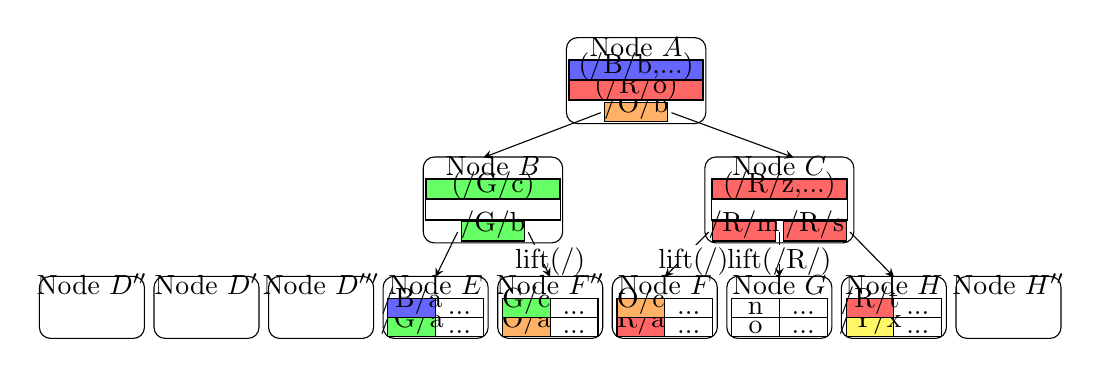
\begin{tikzpicture}
    \node[anchor=south, rectangle, rounded corners, minimum width=.11\textwidth, minimum height=.065\textwidth, draw=black] at (-.005\textwidth, 0) {};
    \node[anchor=south] at (-.005\textwidth, .036\textwidth) {Node $F$};
    \node[anchor=south, rectangle, minimum width=.05\textwidth, minimum height=.02\textwidth, draw=black, fill={red!60}] at (-.03\textwidth, .002\textwidth) {};
    \node[anchor=south] at (-.03\textwidth, -0.005\textwidth) {R/a};
    \node[anchor=south, rectangle, minimum width=.05\textwidth, minimum height=.02\textwidth, draw=black] at (.02\textwidth, .002\textwidth) {};
    \node[anchor=south] at (.02\textwidth, -0.005\textwidth) {...};
    \node[anchor=south, rectangle, minimum width=.05\textwidth, minimum height=.02\textwidth, draw=black, fill={orange!60}] at (-.03\textwidth, .022\textwidth) {};
    \node[anchor=south] at (-.03\textwidth, .015\textwidth) {O/c};
    \node[anchor=south, rectangle, minimum width=.05\textwidth, minimum height=.02\textwidth, draw=black] at (.02\textwidth, .022\textwidth) {};
    \node[anchor=south] at (.02\textwidth, .015\textwidth) {...};

    \node[anchor=south, rectangle, rounded corners, minimum width=.11\textwidth, minimum height=.065\textwidth, draw=black] at (.115\textwidth, 0) {};
    \node[anchor=south] at (.115\textwidth, .036\textwidth) {Node $G$};
    \node[anchor=south, rectangle, minimum width=.05\textwidth, minimum height=.02\textwidth, draw=black] at (.09\textwidth, .002\textwidth) {};
    \node[anchor=south] at (.09\textwidth, -0.005\textwidth) {o};
    \node[anchor=south, rectangle, minimum width=.05\textwidth, minimum height=.02\textwidth, draw=black] at (.14\textwidth, .002\textwidth) {};
    \node[anchor=south] at (.14\textwidth, -0.005\textwidth) {...};
    \node[anchor=south, rectangle, minimum width=.05\textwidth, minimum height=.02\textwidth, draw=black] at (.09\textwidth, .022\textwidth) {};
    \node[anchor=south] at (.09\textwidth, .015\textwidth) {n};
    \node[anchor=south, rectangle, minimum width=.05\textwidth, minimum height=.02\textwidth, draw=black] at (.14\textwidth, .022\textwidth) {};
    \node[anchor=south] at (.14\textwidth, .015\textwidth) {...};

    \node[anchor=south, rectangle, rounded corners, minimum width=.11\textwidth, minimum height=.065\textwidth, draw=black] at (.235\textwidth, 0) {};
    \node[anchor=south] at (.235\textwidth, .036\textwidth) {Node $H$};
    \node[anchor=south, rectangle, minimum width=.05\textwidth, minimum height=.02\textwidth, draw=black, fill={yellow!60}] at (.21\textwidth, .002\textwidth) {};
    \node[anchor=south] at (.21\textwidth, -0.005\textwidth) {/Y/x};
    \node[anchor=south, rectangle, minimum width=.05\textwidth, minimum height=.02\textwidth, draw=black] at (.26\textwidth, .002\textwidth) {};
    \node[anchor=south] at (.26\textwidth, -0.005\textwidth) {...};
    \node[anchor=south, rectangle, minimum width=.05\textwidth, minimum height=.02\textwidth, draw=black, fill={red!60}] at (.21\textwidth, .022\textwidth) {};
    \node[anchor=south] at (.21\textwidth, .015\textwidth) {/R/t};
    \node[anchor=south, rectangle, minimum width=.05\textwidth, minimum height=.02\textwidth, draw=black] at (.26\textwidth, .022\textwidth) {};
    \node[anchor=south] at (.26\textwidth, .015\textwidth) {...};

    \node[anchor=south, rectangle, rounded corners, minimum width=.11\textwidth, minimum height=.065\textwidth, draw=black] at (.355\textwidth, 0) {};
    \node[anchor=south] at (.355\textwidth, .036\textwidth) {Node $H''$};

    \node[anchor=south, rectangle, rounded corners, minimum width=.11\textwidth, minimum height=.065\textwidth, draw=black] at (-.125\textwidth, 0) {};
    \node[anchor=south] at (-.125\textwidth, .036\textwidth) {Node $F''$};
    \node[anchor=south, rectangle, minimum width=.05\textwidth, minimum height=.02\textwidth, draw=black, fill={orange!60}] at (-.15\textwidth, .002\textwidth) {};
    \node[anchor=south] at (-.15\textwidth, -0.005\textwidth) {O/a};
    \node[anchor=south, rectangle, minimum width=.05\textwidth, minimum height=.02\textwidth, draw=black] at (-.1\textwidth, .002\textwidth) {};
    \node[anchor=south] at (-.1\textwidth, -0.005\textwidth) {...};
    \node[anchor=south, rectangle, minimum width=.05\textwidth, minimum height=.02\textwidth, draw=black, fill={green!60}] at (-.15\textwidth, .022\textwidth) {};
    \node[anchor=south] at (-.15\textwidth, .015\textwidth) {G/c};
    \node[anchor=south, rectangle, minimum width=.05\textwidth, minimum height=.02\textwidth, draw=black] at (-.1\textwidth, .022\textwidth) {};
    \node[anchor=south] at (-.1\textwidth, .015\textwidth) {...};

    \node[anchor=south, rectangle, rounded corners, minimum width=.11\textwidth, minimum height=.065\textwidth, draw=black] at (-.245\textwidth, 0) {};
    \node[anchor=south] at (-.245\textwidth, .036\textwidth) {Node $E$};
    \node[anchor=south, rectangle, minimum width=.05\textwidth, minimum height=.02\textwidth, draw=black, fill={green!60}] at (-.27\textwidth, .002\textwidth) {};
    \node[anchor=south] at (-.27\textwidth, -0.005\textwidth) {/G/a};
    \node[anchor=south, rectangle, minimum width=.05\textwidth, minimum height=.02\textwidth, draw=black] at (-.22\textwidth, .002\textwidth) {};
    \node[anchor=south] at (-.22\textwidth, -0.005\textwidth) {...};
    \node[anchor=south, rectangle, minimum width=.05\textwidth, minimum height=.02\textwidth, draw=black, fill={blue!60}] at (-.27\textwidth, .022\textwidth) {};
    \node[anchor=south] at (-.27\textwidth, .015\textwidth) {/B/a};
    \node[anchor=south, rectangle, minimum width=.05\textwidth, minimum height=.02\textwidth, draw=black] at (-.22\textwidth, .022\textwidth) {};
    \node[anchor=south] at (-.22\textwidth, .015\textwidth) {...};

    \node[anchor=south, rectangle, rounded corners, minimum width=.11\textwidth, minimum height=.065\textwidth, draw=black] at (-.365\textwidth, 0) {};
    \node[anchor=south] at (-.365\textwidth, .036\textwidth) {Node $D'''$};

    \node[anchor=south, rectangle, rounded corners, minimum width=.11\textwidth, minimum height=.065\textwidth, draw=black] at (-.485\textwidth, 0) {};
    \node[anchor=south] at (-.485\textwidth, .036\textwidth) {Node $D'$};

    \node[anchor=south, rectangle, rounded corners, minimum width=.11\textwidth, minimum height=.065\textwidth, draw=black] at (-.605\textwidth, 0) {};
    \node[anchor=south] at (-.605\textwidth, .036\textwidth) {Node $D''$};

    \node[anchor=south, rectangle, rounded corners, minimum width=.146\textwidth, minimum height=.09\textwidth, draw=black] at (-.185\textwidth, .1\textwidth) {};
    \node[anchor=south] at (-.185\textwidth, .161\textwidth) {Node $B$};
    \node[anchor=south, rectangle, minimum width=.066\textwidth, minimum height=.02\textwidth, draw=black, fill={green!60}] at (-.185\textwidth, .102\textwidth) {};
    \node[anchor=south] at (-.185\textwidth, .095\textwidth) {/G/b};
    \node[anchor=south, rectangle,minimum width=.142\textwidth, minimum height=.043\textwidth, draw=black] at (-.185\textwidth, .124\textwidth) {};
    \node[anchor=south, rectangle, minimum width=.14\textwidth, minimum height=.02\textwidth, draw=black, fill={green!60}] at (-.185\textwidth, .146\textwidth) {};
    \node[anchor=south] at  (-.185\textwidth, .136\textwidth) {\delm(/G/c)};

    \node[anchor=south, rectangle, rounded corners, minimum width=.156\textwidth, minimum height=.09\textwidth, draw=black] at (.115\textwidth, .1\textwidth) {};
    \node[anchor=south] at (.115\textwidth, .161\textwidth) {Node $C$};
    \node[anchor=south, rectangle, minimum width=.066\textwidth, minimum height=.02\textwidth, draw=black, fill={red!60}] at (.078\textwidth, .102\textwidth) {};
    \node[anchor=south] at (.078\textwidth, .095\textwidth) {/R/m};
    \node[anchor=south, rectangle, minimum width=.066\textwidth, minimum height=.02\textwidth, draw=black, fill={red!60}] at (.152\textwidth, .102\textwidth) {};
    \node[anchor=south] at (.152\textwidth, .095\textwidth) {/R/s};
    \node[anchor=south, rectangle, minimum width=.142\textwidth, minimum height=.043\textwidth, draw=black] at (.115\textwidth, .124\textwidth) {};
    \node[anchor=south, rectangle, minimum width=.14\textwidth, minimum height=.02\textwidth, draw=black, fill={red!60}] at (.115\textwidth, .146\textwidth) {};
    \node[anchor=south] at  (.115\textwidth, .136\textwidth) {\putm(/R/z,...)};

    \node[anchor=south, rectangle, rounded corners, minimum width=.146\textwidth, minimum height=.09\textwidth, draw=black] at (-.035\textwidth, .225\textwidth) {};
    \node[anchor=south] at (-.035\textwidth, .286\textwidth) {Node $A$};
    \node[anchor=south, rectangle, minimum width=.066\textwidth, minimum height=.02\textwidth, draw=black, fill={orange!60}] at (-.035\textwidth, .227\textwidth) {};
    \node[anchor=south] at (-.035\textwidth, .22\textwidth) {/O/b};
    \node[anchor=south, rectangle, minimum width=.142\textwidth, minimum height=.043\textwidth, draw=black] at (-.035\textwidth, .249\textwidth) {};
    \node[anchor=south, rectangle, minimum width=.14\textwidth, minimum height=.02\textwidth, draw=black, fill={red!60}] at (-.035\textwidth, .25\textwidth) {};
    \node[anchor=south] at  (-.035\textwidth, .24\textwidth) {\delm(/R/o)};
    \node[anchor=south, rectangle, minimum width=.14\textwidth, minimum height=.02\textwidth, draw=black, fill={blue!60}] at (-.035\textwidth, .271\textwidth) {};
    \node[anchor=south] at  (-.035\textwidth, .261\textwidth) {\putm(/B/b,...)};

    \draw[->, >=stealth] (-.222\textwidth, .112\textwidth) -- (-.245\textwidth, .065\textwidth);
    \draw[->, >=stealth] (-.148\textwidth, .112\textwidth) -- (-.125\textwidth, .065\textwidth);
    \draw[->, >=stealth] (.041\textwidth, .112\textwidth) -- (-.005\textwidth, .065\textwidth);
    \draw[->, >=stealth] (.115\textwidth, .112\textwidth) -- (.115\textwidth, .065\textwidth);
    \draw[->, >=stealth] (.189\textwidth, .112\textwidth) -- (.235\textwidth, .065\textwidth);
    \draw[->, >=stealth] (-.072\textwidth, .237\textwidth) -- (-.195\textwidth, .19\textwidth);
    \draw[->, >=stealth] (.002\textwidth, .237\textwidth) -- (.13\textwidth, .19\textwidth);

    \node[anchor=north,rectangle, minimum height=.02\textwidth, minimum width=.05\textwidth, fill={white}] at (-.125\textwidth, .099\textwidth) {};
    \node[anchor=north] at (-.125\textwidth, .106\textwidth) {lift(/)};
    \node[anchor=north,rectangle, minimum height=.02\textwidth, minimum width=.05\textwidth, fill={white}] at (.025\textwidth, .099\textwidth) {};
    \node[anchor=north] at (.025\textwidth, .106\textwidth) {lift(/)};
    \node[anchor=north,rectangle, minimum height=.02\textwidth, minimum width=.05\textwidth, fill={white}] at (.115\textwidth, .099\textwidth) {};
    \node[anchor=north] at (.115\textwidth, .106\textwidth) {lift(/R/)};
\end{tikzpicture}

        \caption{\label{subfig:rc-2} The range-clone operation slices out the
            source and destination subtrees.}
    \end{subfigure}
    \begin{subfigure}{\textwidth}
        \centering
        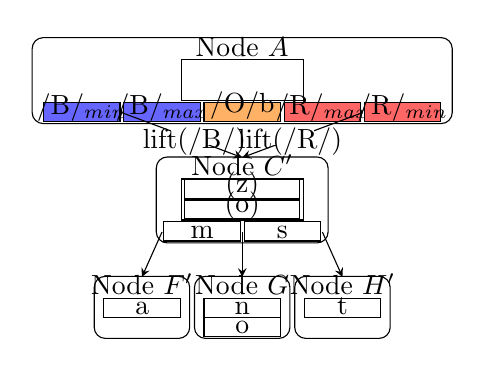
\begin{tikzpicture}
    \node[anchor=south, rectangle, rounded corners, minimum width=.1\textwidth, minimum height=.065\textwidth, draw=black] at (-.105\textwidth, 0) {};
    \node[anchor=south] at (-.105\textwidth, .036\textwidth) {Node $F'$};
    \node[anchor=south, rectangle, minimum width=.08\textwidth, minimum height=.02\textwidth, draw=black] at (-.105\textwidth, .022\textwidth) {};
    \node[anchor=south] at (-.105\textwidth, .015\textwidth) {a};

    \node[anchor=south, rectangle, rounded corners, minimum width=.1\textwidth, minimum height=.065\textwidth, draw=black] at (.0\textwidth, 0) {};
    \node[anchor=south] at (.0\textwidth, .036\textwidth) {Node $G$};
    \node[anchor=south, rectangle, minimum width=.08\textwidth, minimum height=.02\textwidth, draw=black] at (.0\textwidth, .002\textwidth) {};
    \node[anchor=south] at (.0\textwidth, -0.005\textwidth) {o};
    \node[anchor=south, rectangle, minimum width=.08\textwidth, minimum height=.02\textwidth, draw=black] at (.0\textwidth, .022\textwidth) {};
    \node[anchor=south] at (.0\textwidth, .015\textwidth) {n};

    \node[anchor=south, rectangle, rounded corners, minimum width=.1\textwidth, minimum height=.065\textwidth, draw=black] at (.105\textwidth, 0) {};
    \node[anchor=south] at (.105\textwidth, .036\textwidth) {Node $H'$};
    \node[anchor=south, rectangle, minimum width=.08\textwidth, minimum height=.02\textwidth, draw=black] at (.105\textwidth, .022\textwidth) {};
    \node[anchor=south] at (.105\textwidth, .015\textwidth) {t};

    \node[anchor=south, rectangle, rounded corners, minimum width=.18\textwidth, minimum height=.09\textwidth, draw=black] at (.0\textwidth, .1\textwidth) {};
    \node[anchor=south] at (.0\textwidth, .161\textwidth) {Node $C'$};
    \node[anchor=south, rectangle, minimum width=.08\textwidth, minimum height=.02\textwidth, draw=black] at (-.042\textwidth, .102\textwidth) {};
    \node[anchor=south] at (-.042\textwidth, .095\textwidth) {m};
    \node[anchor=south, rectangle, minimum width=.08\textwidth, minimum height=.02\textwidth, draw=black] at (.042\textwidth, .102\textwidth) {};
    \node[anchor=south] at (.042\textwidth, .095\textwidth) {s};
    \node[anchor=south, rectangle, minimum width=.128\textwidth, minimum height=.043\textwidth, draw=black] at (.0\textwidth, .124\textwidth) {};
    \node[anchor=south, rectangle, minimum width=.12\textwidth, minimum height=.02\textwidth, draw=black] at (.0\textwidth, .146\textwidth) {};
    \node[anchor=south] at  (.0\textwidth, .136\textwidth) {\putm(z)};
    \node[anchor=south, rectangle, minimum width=.12\textwidth, minimum height=.02\textwidth, draw=black] at (.0\textwidth, .125\textwidth) {};
    \node[anchor=south] at  (.0\textwidth, .115\textwidth) {\delm(o)};

    \node[anchor=south, rectangle, rounded corners, minimum width=.44\textwidth, minimum height=.09\textwidth, draw=black] at (.0\textwidth, .225\textwidth) {};
    \node[anchor=south] at (.0\textwidth, .286\textwidth) {Node $A$};
    \node[anchor=south, rectangle, minimum width=.08\textwidth, minimum height=.02\textwidth, draw=black, fill={blue!60}] at (-.168\textwidth, .227\textwidth) {};
    \node[anchor=south] at (-.168\textwidth, .218\textwidth) {/B/$_{min}$};
    \node[anchor=south, rectangle, minimum width=.08\textwidth, minimum height=.02\textwidth, draw=black, fill={blue!60}] at (-.084\textwidth, .227\textwidth) {};
    \node[anchor=south] at (-.084\textwidth, .218\textwidth) {/B/$_{max}$};
    \node[anchor=south, rectangle, minimum width=.08\textwidth, minimum height=.02\textwidth, draw=black, fill={orange!60}] at (.0\textwidth, .227\textwidth) {};
    \node[anchor=south] at (.0\textwidth, .22\textwidth) {/O/b};
    \node[anchor=south, rectangle, minimum width=.08\textwidth, minimum height=.02\textwidth, draw=black, fill={red!60}] at (.084\textwidth, .227\textwidth) {};
    \node[anchor=south] at (.084\textwidth, .218\textwidth) {/R/$_{max}$};
    \node[anchor=south, rectangle, minimum width=.08\textwidth, minimum height=.02\textwidth, draw=black, fill={red!60}] at (.168\textwidth, .227\textwidth) {};
    \node[anchor=south] at (.168\textwidth, .218\textwidth) {/R/$_{min}$};
    \node[anchor=south, rectangle, minimum width=.128\textwidth, minimum height=.043\textwidth, draw=black] at (.0\textwidth, .249\textwidth) {};

    \draw[->, >=stealth] (-.084\textwidth, .112\textwidth) -- (-.105\textwidth, .065\textwidth);
    \draw[->, >=stealth] (.0\textwidth, .112\textwidth) -- (.0\textwidth, .065\textwidth);
    \draw[->, >=stealth] (.084\textwidth, .112\textwidth) -- (.105\textwidth, .065\textwidth);
    \draw[->, >=stealth] (-.126\textwidth, .237\textwidth) -- (.0\textwidth, .19\textwidth);
    \draw[->, >=stealth] (.126\textwidth, .237\textwidth) -- (.0\textwidth, .19\textwidth);

    \node[anchor=north,rectangle, minimum height=.02\textwidth, minimum width=.05\textwidth, fill={white}] at (-.05\textwidth, .224\textwidth) {};
    \node[anchor=north] at (-.05\textwidth, .231\textwidth) {lift(/B/)};
    \node[anchor=north,rectangle, minimum height=.02\textwidth, minimum width=.05\textwidth, fill={white}] at (.05\textwidth, .224\textwidth) {};
    \node[anchor=north] at (.05\textwidth, .231\textwidth) {lift(/R/)};
\end{tikzpicture}

        \caption{\label{subfig:rc-3} The range-clone operations shares the source
            subtree at both source and destination and garbage-collects the
            destination subtree.}
    \end{subfigure}
    \caption[All operations in range-clone]{\label{fig:rc}
        An example of range-clone(``/R/'', ``/B/'') that completes all work
        in the critical path.}
\end{figure}

The range-clone operation can be implemented in the \bet by modifying the
range-rename operation.
In particular, after slicing out the source and destination subtrees with tree
surgery,
instead of swapping the two subtrees and injecting a range-delete message
for source keys in a range-rename operation,
a range-clone operation can share the source subtree in both source and
destination,
and garbage collect the destination subtree.

Figure~\ref{fig:rc} shows an example of performing the work of
range-clone(``/R/'', ``/B/'') on the lifted \bet in Figure~\ref{subfig:rc-1}.
Figure~\ref{subfig:rc-2} shows the lifted \bet after tree surgery.
Tree surgery slices out the source and destination subtrees,
after flushing pending messages to the LCAs.
This tree surgery is completely identical to that in the range-rename operation
(Figure~\ref{subfig:rr-2}).
In Figure~\ref{subfig:rc-3}, the lifted \bet garbage collects the destination
subtree, rooted at Node $B'$, and sets the parent-to-child pointer between
``/B/$_{min}$'' and ``/B/$_{max}$''
(``/B/$_{min}$'' and ``/B/$_{max}$'' are the minimum and maximum keys with
prefix ``/B/'', respectively)
to Node $C'$,
which is the root node of the source subtree.

The subtree rooted at Node $C'$ is now shared by two parent-to-child pointers,
and queries for
both ``/B/'' and ``/R/'' keys will fetch messages and key/value pairs in that
subtree.
However, because queries need to reconstruct the key by prepending lifted
prefixes on the root-to-leaf path, they get different keys following different
parent-to-child pointers.

Sharing a subtree among multiple parent-to-child pointers transforms a lifted
\bet into a lifted \bedag (Directed Acyclic Graph) with some constraints.
Because the \bedag is generated by sharing subtrees in a \bet,
there is still one root node in the \bedag,
which can reach all nodes in the \bedag through parent-to-child pointers.
And since the source and destination subtrees generated by tree surgery are at
the same height, the length of any root-to-leaf path in the \bedag is still
logarithmic in the size of the graph.

The lifted \bedag adds reference counts for \bet nodes to track the sharing
status.
In particular, \fti has a node table that a maps node ID to
the actual location of the node.
We store the reference count of each node in the node table alongside
the mapping.
Before flushing to a node, the \bedag must check the reference count of the node.
A reference count greater than 1 means the node is shared by multiple
parent-to-child pointers.
The lifted \bedag must break the sharing because other paths should not see the
messages this flush is going to inject into the node.

In a lifted \bedag, the root-to-leaf traversals of different queries may end up
reaching the same leaf node, fetching the same key/value pair.
However, because key lifting requires queries to reconstruct the full key by
concatenating lifted prefixes, different queries treat the same key/value pairs
with different prefixes.
For example, in Figure~\ref{subfig:rc-3}, queries for key ``/R/n'' and ``/B/n''
follow the same root-to-leaf path and get the same key/value pair from the
leaf node, Node $G$.
However, when walking down the tree from Node $A$ to Node $C$, the query for
key ``/R/n'' follows the parent-to-child pointer that lifts prefix ``/R/''.
Therefore, it gets key ``/R/n'' after prepending lifted prefixes along the
root-to-leaf path.
Similarly, the query for key ``/B/n'' gets a result with key ``/B/n''.

The lifted \bedag must break the sharing of a node when flushing messages
through one of its parent-to-child pointer.
Because these messages are injected into the tree after the range-clone
operation, they are not shared by all parent-to-child pointers.
Thus, the node can no longer be shared by multiple parents after flushing.
However, before accumulating enough messages to flush to the subtree,
the subtree is shared by multiple parent-to-child pointers,
which saves a lot of space compared to the naive approach that clones
the source subtree in the range-clone operation.

The lifted \bedag breaks the sharing of a node using Copy-on-Write (CoW).
For instance, after the range-clone operation, one parent of the shared node
might choose to flush its messages to the node.
At this moment, the lifted \bedag creates a new node that is identical to the
shared node, sharing the content and all children of the node.
The lifted \bedag then sets the parent-to-child pointer in the parent to the new
node and performs the flush.

\begin{figure}
    \begin{subfigure}{\textwidth}
        \centering
        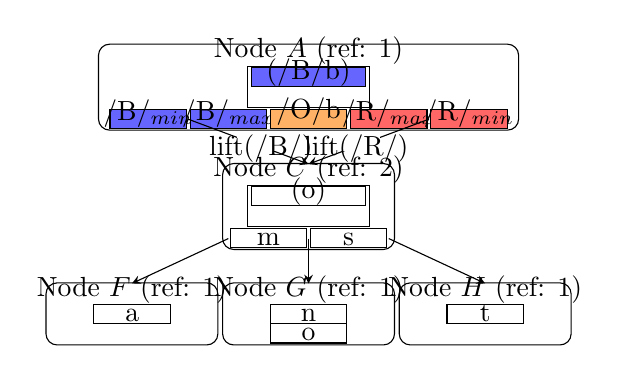
\begin{tikzpicture}
    \node[anchor=south, rectangle, rounded corners, minimum width=.18\textwidth, minimum height=.065\textwidth, draw=black] at (-.185\textwidth, 0) {};
    \node[anchor=south] at (-.185\textwidth, .034\textwidth) {Node $F$ (ref: 1)};
    \node[anchor=south, rectangle, minimum width=.08\textwidth, minimum height=.02\textwidth, draw=black] at (-.185\textwidth, .022\textwidth) {};
    \node[anchor=south] at (-.185\textwidth, .015\textwidth) {a};

    \node[anchor=south, rectangle, rounded corners, minimum width=.18\textwidth, minimum height=.065\textwidth, draw=black] at (.0\textwidth, 0) {};
    \node[anchor=south] at (.0\textwidth, .034\textwidth) {Node $G$ (ref: 1)};
    \node[anchor=south, rectangle, minimum width=.08\textwidth, minimum height=.02\textwidth, draw=black] at (.0\textwidth, .002\textwidth) {};
    \node[anchor=south] at (.0\textwidth, -0.005\textwidth) {o};
    \node[anchor=south, rectangle, minimum width=.08\textwidth, minimum height=.02\textwidth, draw=black] at (.0\textwidth, .022\textwidth) {};
    \node[anchor=south] at (.0\textwidth, .015\textwidth) {n};

    \node[anchor=south, rectangle, rounded corners, minimum width=.18\textwidth, minimum height=.065\textwidth, draw=black] at (.185\textwidth, 0) {};
    \node[anchor=south] at (.185\textwidth, .034\textwidth) {Node $H$ (ref: 1)};
    \node[anchor=south, rectangle, minimum width=.08\textwidth, minimum height=.02\textwidth, draw=black] at (.185\textwidth, .022\textwidth) {};
    \node[anchor=south] at (.185\textwidth, .015\textwidth) {t};

    \node[anchor=south, rectangle, rounded corners, minimum width=.18\textwidth, minimum height=.09\textwidth, draw=black] at (.0\textwidth, .1\textwidth) {};
    \node[anchor=south] at (.0\textwidth, .159\textwidth) {Node $C$ (ref: 2)};
    \node[anchor=south, rectangle, minimum width=.08\textwidth, minimum height=.02\textwidth, draw=black] at (-.042\textwidth, .102\textwidth) {};
    \node[anchor=south] at (-.042\textwidth, .095\textwidth) {m};
    \node[anchor=south, rectangle, minimum width=.08\textwidth, minimum height=.02\textwidth, draw=black] at (.042\textwidth, .102\textwidth) {};
    \node[anchor=south] at (.042\textwidth, .095\textwidth) {s};
    \node[anchor=south, rectangle, minimum width=.128\textwidth, minimum height=.043\textwidth, draw=black] at (.0\textwidth, .124\textwidth) {};
    \node[anchor=south, rectangle, minimum width=.12\textwidth, minimum height=.02\textwidth, draw=black] at (.0\textwidth, .146\textwidth) {};
    \node[anchor=south] at  (.0\textwidth, .136\textwidth) {\delm(o)};

    \node[anchor=south, rectangle, rounded corners, minimum width=.44\textwidth, minimum height=.09\textwidth, draw=black] at (.0\textwidth, .225\textwidth) {};
    \node[anchor=south] at (.0\textwidth, .284\textwidth) {Node $A$ (ref: 1)};
    \node[anchor=south, rectangle, minimum width=.08\textwidth, minimum height=.02\textwidth, draw=black, fill={blue!60}] at (-.168\textwidth, .227\textwidth) {};
    \node[anchor=south] at (-.168\textwidth, .218\textwidth) {/B/$_{min}$};
    \node[anchor=south, rectangle, minimum width=.08\textwidth, minimum height=.02\textwidth, draw=black, fill={blue!60}] at (-.084\textwidth, .227\textwidth) {};
    \node[anchor=south] at (-.084\textwidth, .218\textwidth) {/B/$_{max}$};
    \node[anchor=south, rectangle, minimum width=.08\textwidth, minimum height=.02\textwidth, draw=black, fill={orange!60}] at (.0\textwidth, .227\textwidth) {};
    \node[anchor=south] at (.0\textwidth, .22\textwidth) {/O/b};
    \node[anchor=south, rectangle, minimum width=.08\textwidth, minimum height=.02\textwidth, draw=black, fill={red!60}] at (.084\textwidth, .227\textwidth) {};
    \node[anchor=south] at (.084\textwidth, .218\textwidth) {/R/$_{max}$};
    \node[anchor=south, rectangle, minimum width=.08\textwidth, minimum height=.02\textwidth, draw=black, fill={red!60}] at (.168\textwidth, .227\textwidth) {};
    \node[anchor=south] at (.168\textwidth, .218\textwidth) {/R/$_{min}$};
    \node[anchor=south, rectangle, minimum width=.128\textwidth, minimum height=.043\textwidth, draw=black] at (.0\textwidth, .249\textwidth) {};
    \node[anchor=south, rectangle, minimum width=.12\textwidth, minimum height=.02\textwidth, draw=black, fill={blue!60}] at (.0\textwidth, .271\textwidth) {};
    \node[anchor=south] at  (.0\textwidth, .261\textwidth) {\putm(/B/b)};

    \draw[->, >=stealth] (-.084\textwidth, .112\textwidth) -- (-.185\textwidth, .065\textwidth);
    \draw[->, >=stealth] (.0\textwidth, .112\textwidth) -- (.0\textwidth, .065\textwidth);
    \draw[->, >=stealth] (.084\textwidth, .112\textwidth) -- (.185\textwidth, .065\textwidth);
    \draw[->, >=stealth] (-.126\textwidth, .237\textwidth) -- (.0\textwidth, .19\textwidth);
    \draw[->, >=stealth] (.126\textwidth, .237\textwidth) -- (.0\textwidth, .19\textwidth);

    \node[anchor=north,rectangle, minimum height=.02\textwidth, minimum width=.05\textwidth, fill={white}] at (-.05\textwidth, .224\textwidth) {};
    \node[anchor=north] at (-.05\textwidth, .231\textwidth) {lift(/B/)};
    \node[anchor=north,rectangle, minimum height=.02\textwidth, minimum width=.05\textwidth, fill={white}] at (.05\textwidth, .224\textwidth) {};
    \node[anchor=north] at (.05\textwidth, .231\textwidth) {lift(/R/)};
\end{tikzpicture}

        \caption{\label{subfig:cow-1} Node $C$ is a shared by two
            parent-to-child pointers in Node $A$.}
    \end{subfigure}
    \begin{subfigure}{\textwidth}
        \centering
        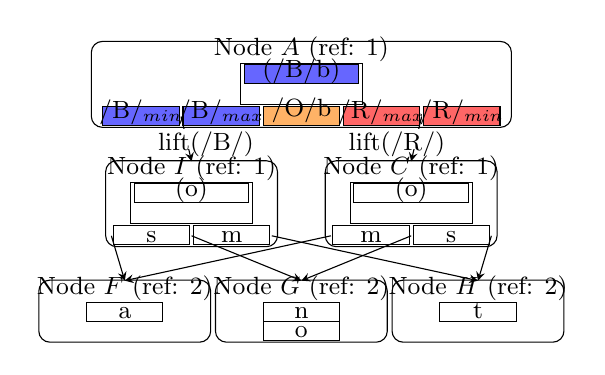
\begin{tikzpicture}
    \node[anchor=south, rectangle, rounded corners, minimum width=.18\textwidth, minimum height=.065\textwidth, draw=black] at (-.185\textwidth, 0) {};
    \node[anchor=south, font=\small] at (-.185\textwidth, .034\textwidth) {Node $F$ (ref: 2)};
    \node[anchor=south, rectangle, minimum width=.08\textwidth, minimum height=.02\textwidth, draw=black] at (-.185\textwidth, .022\textwidth) {};
    \node[anchor=south, font=\small] at (-.185\textwidth, .015\textwidth) {a};

    \node[anchor=south, rectangle, rounded corners, minimum width=.18\textwidth, minimum height=.065\textwidth, draw=black] at (.0\textwidth, 0) {};
    \node[anchor=south, font=\small] at (.0\textwidth, .034\textwidth) {Node $G$ (ref: 2)};
    \node[anchor=south, rectangle, minimum width=.08\textwidth, minimum height=.02\textwidth, draw=black] at (.0\textwidth, .002\textwidth) {};
    \node[anchor=south, font=\small] at (.0\textwidth, -0.005\textwidth) {o};
    \node[anchor=south, rectangle, minimum width=.08\textwidth, minimum height=.02\textwidth, draw=black] at (.0\textwidth, .022\textwidth) {};
    \node[anchor=south, font=\small] at (.0\textwidth, .015\textwidth) {n};

    \node[anchor=south, rectangle, rounded corners, minimum width=.18\textwidth, minimum height=.065\textwidth, draw=black] at (.185\textwidth, 0) {};
    \node[anchor=south, font=\small] at (.185\textwidth, .034\textwidth) {Node $H$ (ref: 2)};
    \node[anchor=south, rectangle, minimum width=.08\textwidth, minimum height=.02\textwidth, draw=black] at (.185\textwidth, .022\textwidth) {};
    \node[anchor=south, font=\small] at (.185\textwidth, .015\textwidth) {t};

    \node[anchor=south, rectangle, rounded corners, minimum width=.18\textwidth, minimum height=.09\textwidth, draw=black] at (-.115\textwidth, .1\textwidth) {};
    \node[anchor=south, font=\small] at (-.115\textwidth, .159\textwidth) {Node $I$ (ref: 1)};
    \node[anchor=south, rectangle, minimum width=.08\textwidth, minimum height=.02\textwidth, draw=black] at (-.073\textwidth, .102\textwidth) {};
    \node[anchor=south, font=\small] at (-.073\textwidth, .095\textwidth) {m};
    \node[anchor=south, rectangle, minimum width=.08\textwidth, minimum height=.02\textwidth, draw=black] at (-.157\textwidth, .102\textwidth) {};
    \node[anchor=south, font=\small] at (-.157\textwidth, .095\textwidth) {s};
    \node[anchor=south, rectangle, minimum width=.128\textwidth, minimum height=.043\textwidth, draw=black] at (-.115\textwidth, .124\textwidth) {};
    \node[anchor=south, rectangle, minimum width=.12\textwidth, minimum height=.02\textwidth, draw=black] at (-.115\textwidth, .146\textwidth) {};
    \node[anchor=south, font=\small] at  (-.115\textwidth, .136\textwidth) {\delm(o)};

    \node[anchor=south, rectangle, rounded corners, minimum width=.18\textwidth, minimum height=.09\textwidth, draw=black] at (.115\textwidth, .1\textwidth) {};
    \node[anchor=south, font=\small] at (.115\textwidth, .159\textwidth) {Node $C$ (ref: 1)};
    \node[anchor=south, rectangle, minimum width=.08\textwidth, minimum height=.02\textwidth, draw=black] at (.073\textwidth, .102\textwidth) {};
    \node[anchor=south, font=\small] at (.073\textwidth, .095\textwidth) {m};
    \node[anchor=south, rectangle, minimum width=.08\textwidth, minimum height=.02\textwidth, draw=black] at (.157\textwidth, .102\textwidth) {};
    \node[anchor=south, font=\small] at (.157\textwidth, .095\textwidth) {s};
    \node[anchor=south, rectangle, minimum width=.128\textwidth, minimum height=.043\textwidth, draw=black] at (.115\textwidth, .124\textwidth) {};
    \node[anchor=south, rectangle, minimum width=.12\textwidth, minimum height=.02\textwidth, draw=black] at (.115\textwidth, .146\textwidth) {};
    \node[anchor=south, font=\small] at  (.115\textwidth, .136\textwidth) {\delm(o)};

    \node[anchor=south, rectangle, rounded corners, minimum width=.44\textwidth, minimum height=.09\textwidth, draw=black] at (.0\textwidth, .225\textwidth) {};
    \node[anchor=south, font=\small] at (.0\textwidth, .284\textwidth) {Node $A$ (ref: 1)};
    \node[anchor=south, rectangle, minimum width=.08\textwidth, minimum height=.02\textwidth, draw=black, fill={blue!60}] at (-.168\textwidth, .227\textwidth) {};
    \node[anchor=south, font=\small] at (-.168\textwidth, .218\textwidth) {/B/$_{min}$};
    \node[anchor=south, rectangle, minimum width=.08\textwidth, minimum height=.02\textwidth, draw=black, fill={blue!60}] at (-.084\textwidth, .227\textwidth) {};
    \node[anchor=south, font=\small] at (-.084\textwidth, .218\textwidth) {/B/$_{max}$};
    \node[anchor=south, rectangle, minimum width=.08\textwidth, minimum height=.02\textwidth, draw=black, fill={orange!60}] at (.0\textwidth, .227\textwidth) {};
    \node[anchor=south, font=\small] at (.0\textwidth, .22\textwidth) {/O/b};
    \node[anchor=south, rectangle, minimum width=.08\textwidth, minimum height=.02\textwidth, draw=black, fill={red!60}] at (.084\textwidth, .227\textwidth) {};
    \node[anchor=south, font=\small] at (.084\textwidth, .218\textwidth) {/R/$_{max}$};
    \node[anchor=south, rectangle, minimum width=.08\textwidth, minimum height=.02\textwidth, draw=black, fill={red!60}] at (.168\textwidth, .227\textwidth) {};
    \node[anchor=south, font=\small] at (.168\textwidth, .218\textwidth) {/R/$_{min}$};
    \node[anchor=south, rectangle, minimum width=.128\textwidth, minimum height=.043\textwidth, draw=black] at (.0\textwidth, .249\textwidth) {};
    \node[anchor=south, rectangle, minimum width=.12\textwidth, minimum height=.02\textwidth, draw=black, fill={blue!60}] at (.0\textwidth, .271\textwidth) {};
    \node[anchor=south, font=\small] at  (.0\textwidth, .261\textwidth) {\putm(/B/b)};

    \draw[->, >=stealth] (-.199\textwidth, .112\textwidth) -- (-.185\textwidth, .065\textwidth);
    \draw[->, >=stealth] (-.115\textwidth, .112\textwidth) -- (.0\textwidth, .065\textwidth);
    \draw[->, >=stealth] (-.031\textwidth, .112\textwidth) -- (.185\textwidth, .065\textwidth);
    \draw[->, >=stealth] (.031\textwidth, .112\textwidth) -- (-.185\textwidth, .065\textwidth);
    \draw[->, >=stealth] (.115\textwidth, .112\textwidth) -- (.0\textwidth, .065\textwidth);
    \draw[->, >=stealth] (.199\textwidth, .112\textwidth) -- (.185\textwidth, .065\textwidth);
    \draw[->, >=stealth] (-.126\textwidth, .237\textwidth) -- (-.115\textwidth, .19\textwidth);
    \draw[->, >=stealth] (.126\textwidth, .237\textwidth) -- (.115\textwidth, .19\textwidth);

    \node[anchor=north,rectangle, minimum height=.02\textwidth, minimum width=.05\textwidth, fill={white}] at (-.1\textwidth, .224\textwidth) {};
    \node[anchor=north, font=\small] at (-.1\textwidth, .231\textwidth) {lift(/B/)};
    \node[anchor=north,rectangle, minimum height=.02\textwidth, minimum width=.05\textwidth, fill={white}] at (.1\textwidth, .224\textwidth) {};
    \node[anchor=north, font=\small] at (.1\textwidth, .231\textwidth) {lift(/R/)};
\end{tikzpicture}

        \caption{\label{subfig:cow-2} Before Node $A$ flushes ``/B/'' messages,
        it breaks the sharing by cloning Node $C$ to Node $I$.}
    \end{subfigure}
    \caption[\bedags break node sharing with CoW]{\label{fig:cow}
        When a parent want to flush messages to a shared node,
        it breaks the sharing by cloning the shared node.}
\end{figure}

Figure~\ref{fig:cow} shows an example of the CoW process.
In this example, we also show the reference count of a node alongside the node
ID.
In Figure~\ref{subfig:cow-1}, Node $A$ has two parent-to-child pointers to
Node $C$.
Therefore, the reference count of Node $C$ is 2 and
Node $F$, $G$ and $H$ have reference count 1.
When Node $A$ wants to flush messages with through the parent-to-child pointer
between ``/B/$_{min}$'' and ``/B/$_{max}$'',
the flushing process finds out that Node $C$ is a shared node because its
reference count is greater than 1.
Therefore, it clones Node $C$ to break the sharing.
As shown in Figure~\ref{subfig:cow-2}, the \bedag creates a new node, Node $I$,
that is identical to Node $C$.
Now, both Node $C$ and $I$ have reference count 1, while Node $F$, $G$, and
$H$ have reference count 2.
With the sharing broken, the \bedag can flush message \putm(``/B/b'',...) from
Node $A$ to Node $I$ without affecting the other root-to-leaf path that
includes Node $C$.

\subsection{Range-clone with \goto messages}
\label{sec:rc:goto}

Instead of completing all work on the critical path, range-clone can use a
new type of message, the \goto message, that delays tree surgery
in the lifted \bedag.

This subsection describes the \goto message and how the range-clone operation
can return to the user by injecting a \goto message into the root node.
The next subsection (Section~\ref{sec:rc:flush}) shows how the \bet flushes
a \goto message,
completing all work in the range-clone operation.

\paragraph{The \goto message.}
A \goto message consists of 3 parts: a \dpre, a \spre, a node ID
(with its height in the \bedag).
Generally speaking, a \goto message serves as an additional parent-to-child
pointer in the \bet node with an \xf (translate-and-filter) function.
Rather than following normal parent-to-child pointers in the node,
a query whose search key falls in the key range (\dpre$_{min}$, \dpre$_{max}$)
must follow the \goto message, that is, the next node the query visits
should be the node whose node ID is in the \goto message.
Also, the query should update its search key by replacing prefix \dpre with
prefix \spre.
Later, the query needs to reconstruct the result by replacing prefix \spre
with prefix \dpre in the key.
Therefore, the \goto message should filter out keys that are not in the
key range (\spre$_{min}$, \spre$_{max}$) in the subsequent search.

\begin{figure}
    \begin{subfigure}{\textwidth}
        \centering
        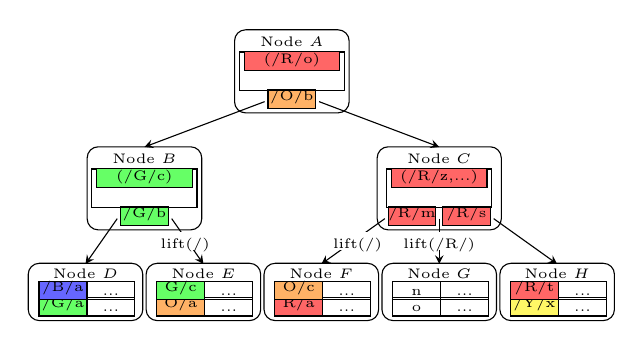
\begin{tikzpicture}[xscale=0.95, yscale=0.95]
            \node[anchor=south, rectangle, rounded corners, minimum height=.06\textwidth, minimum width=.12\textwidth, draw=black] at (0, 0) {};
            \node[anchor=south, font=\tiny] at (0, .036\textwidth) {Node $F$};
            \node[anchor=south, rectangle, minimum height=.015\textwidth, minimum width=.05\textwidth, draw=black, fill={red!60}] at (-.025\textwidth, .005\textwidth) {};
            \node[anchor=south, font=\tiny] at (-.025\textwidth, 0) {R/a};
            \node[anchor=south, rectangle, minimum height=.015\textwidth, minimum width=.05\textwidth, draw=black] at (.028\textwidth, .005\textwidth) {};
            \node[anchor=south, font=\tiny] at (.028\textwidth, 0) {...};
            \node[anchor=south, rectangle, minimum height=.015\textwidth, minimum width=.05\textwidth, draw=black, fill={orange!60}] at (-.025\textwidth, .023\textwidth) {};
            \node[anchor=south, font=\tiny] at (-.025\textwidth, .018\textwidth) {O/c};
            \node[anchor=south, rectangle, minimum height=.015\textwidth, minimum width=.05\textwidth, draw=black] at (.028\textwidth, .023\textwidth) {};
            \node[anchor=south, font=\tiny] at (.028\textwidth, .018\textwidth) {...};

            \node[anchor=south, rectangle, rounded corners, minimum height=.06\textwidth, minimum width=.12\textwidth, draw=black] at (.13\textwidth, 0) {};
            \node[anchor=south, font=\tiny] at (.13\textwidth, .036\textwidth) {Node $G$};
            \node[anchor=south, rectangle, minimum height=.015\textwidth, minimum width=.05\textwidth, draw=black] at (.105\textwidth, .005\textwidth) {};
            \node[anchor=south, font=\tiny] at (.105\textwidth, 0) {o};
            \node[anchor=south, rectangle, minimum height=.015\textwidth, minimum width=.05\textwidth, draw=black] at (.158\textwidth, .005\textwidth) {};
            \node[anchor=south, font=\tiny] at (.158\textwidth, 0) {...};
            \node[anchor=south, rectangle, minimum height=.015\textwidth, minimum width=.05\textwidth, draw=black] at (.105\textwidth, .023\textwidth) {};
            \node[anchor=south, font=\tiny] at (.105\textwidth, .018\textwidth) {n};
            \node[anchor=south, rectangle, minimum height=.015\textwidth, minimum width=.05\textwidth, draw=black] at (.158\textwidth, .023\textwidth) {};
            \node[anchor=south, font=\tiny] at (.158\textwidth, .018\textwidth) {...};

            \node[anchor=south, rectangle, rounded corners, minimum height=.06\textwidth, minimum width=.12\textwidth, draw=black] at (.26\textwidth, 0) {};
            \node[anchor=south, font=\tiny] at (.26\textwidth, .036\textwidth) {Node $H$};
            \node[anchor=south, rectangle, minimum height=.015\textwidth, minimum width=.05\textwidth, draw=black, fill={yellow!60}] at (.235\textwidth, .005\textwidth) {};
            \node[anchor=south, font=\tiny] at (.235\textwidth, 0) {/Y/x};
            \node[anchor=south, rectangle, minimum height=.015\textwidth, minimum width=.05\textwidth, draw=black] at (.288\textwidth, .005\textwidth) {};
            \node[anchor=south, font=\tiny] at (.288\textwidth, 0) {...};
            \node[anchor=south, rectangle, minimum height=.015\textwidth, minimum width=.05\textwidth, draw=black, fill={red!60}] at (.235\textwidth, .023\textwidth) {};
            \node[anchor=south, font=\tiny] at (.235\textwidth, .018\textwidth) {/R/t};
            \node[anchor=south, rectangle, minimum height=.015\textwidth, minimum width=.05\textwidth, draw=black] at (.288\textwidth, .023\textwidth) {};
            \node[anchor=south, font=\tiny] at (.288\textwidth, .018\textwidth) {...};

            \node[anchor=south, rectangle, rounded corners, minimum height=.06\textwidth, minimum width=.12\textwidth, draw=black] at (-.13\textwidth, 0) {};
            \node[anchor=south, font=\tiny] at (-.13\textwidth, .036\textwidth) {Node $E$};
            \node[anchor=south, rectangle, minimum height=.015\textwidth, minimum width=.05\textwidth, draw=black, fill={orange!60}] at (-.155\textwidth, .005\textwidth) {};
            \node[anchor=south, font=\tiny] at (-.155\textwidth, 0) {O/a};
            \node[anchor=south, rectangle, minimum height=.015\textwidth, minimum width=.05\textwidth, draw=black] at (-.102\textwidth, .005\textwidth) {};
            \node[anchor=south, font=\tiny] at (-.102\textwidth, 0) {...};
            \node[anchor=south, rectangle, minimum height=.015\textwidth, minimum width=.05\textwidth, draw=black, fill={green!60}] at (-.155\textwidth, .023\textwidth) {};
            \node[anchor=south, font=\tiny] at (-.155\textwidth, .018\textwidth) {G/c};
            \node[anchor=south, rectangle, minimum height=.015\textwidth, minimum width=.05\textwidth, draw=black] at (-.102\textwidth, .023\textwidth) {};
            \node[anchor=south, font=\tiny] at (-.102\textwidth, .018\textwidth) {...};

            \node[anchor=south, rectangle, rounded corners, minimum height=.06\textwidth, minimum width=.12\textwidth, draw=black] at (-.26\textwidth, 0) {};
            \node[anchor=south, font=\tiny] at (-.26\textwidth, .036\textwidth) {Node $D$};
            \node[anchor=south, rectangle, minimum height=.015\textwidth, minimum width=.05\textwidth, draw=black, fill={green!60}] at (-.285\textwidth, .005\textwidth) {};
            \node[anchor=south, font=\tiny] at (-.285\textwidth, 0) {/G/a};
            \node[anchor=south, rectangle, minimum height=.015\textwidth, minimum width=.05\textwidth, draw=black] at (-.232\textwidth, .005\textwidth) {};
            \node[anchor=south, font=\tiny] at (-.232\textwidth, 0) {...};
            \node[anchor=south, rectangle, minimum height=.015\textwidth, minimum width=.05\textwidth, draw=black, fill={blue!60}] at (-.285\textwidth, .023\textwidth) {};
            \node[anchor=south, font=\tiny] at (-.285\textwidth, .018\textwidth) {/B/a};
            \node[anchor=south, rectangle, minimum height=.015\textwidth, minimum width=.05\textwidth, draw=black] at (-.232\textwidth, .023\textwidth) {};
            \node[anchor=south, font=\tiny] at (-.232\textwidth, .018\textwidth) {...};

            \node[anchor=south, rectangle, rounded corners, minimum height=.087\textwidth, minimum width=.12\textwidth, draw=black] at (-.195\textwidth, .1\textwidth) {};
            \node[anchor=south, font=\tiny] at (-.195\textwidth, .163\textwidth) {Node $B$};
            \node[anchor=south, rectangle, minimum height=.015\textwidth, minimum width=.05\textwidth, draw=black, fill={green!60}] at (-.195\textwidth, .105\textwidth) {};
            \node[anchor=south, font=\tiny] at (-.195\textwidth, .1\textwidth) {/G/b};
            \node[anchor=south, rectangle, minimum height=.04\textwidth, minimum width=.11\textwidth, draw=black] at (-.195\textwidth, .125\textwidth) {};
            \node[anchor=south, rectangle, minimum height=.015\textwidth, minimum width=.1\textwidth, draw=black, fill={green!60}] at (-.195\textwidth, .147\textwidth) {};
            \node[anchor=south, font=\tiny] at  (-.195\textwidth, .141\textwidth) {\delm(/G/c)};

            \node[anchor=south, rectangle, rounded corners, minimum height=.087\textwidth, minimum width=.13\textwidth, draw=black] at (.13\textwidth, .1\textwidth) {};
            \node[anchor=south, font=\tiny] at (.13\textwidth, .163\textwidth) {Node $C$};
            \node[anchor=south, rectangle, minimum height=.015\textwidth, minimum width=.05\textwidth, draw=black, fill={red!60}] at (.1\textwidth, .105\textwidth) {};
            \node[anchor=south, font=\tiny] at (.1\textwidth, .1\textwidth) {/R/m};
            \node[anchor=south, rectangle, minimum height=.015\textwidth, minimum width=.05\textwidth, draw=black, fill={red!60}] at (.16\textwidth, .105\textwidth) {};
            \node[anchor=south, font=\tiny] at (.16\textwidth, .1\textwidth) {/R/s};
            \node[anchor=south, rectangle, minimum height=.04\textwidth, minimum width=.11\textwidth, draw=black] at (.13\textwidth, .125\textwidth) {};
            \node[anchor=south, rectangle, minimum height=.015\textwidth, minimum width=.1\textwidth, draw=black, fill={red!60}] at (.13\textwidth, .147\textwidth) {};
            \node[anchor=south, font=\tiny] at  (.13\textwidth, .141\textwidth) {\putm(/R/z,...)};

            \node[anchor=south, rectangle, rounded corners, minimum height=.087\textwidth, minimum width=.12\textwidth, draw=black] at (-.0325\textwidth, .229\textwidth) {};
            \node[anchor=south, font=\tiny] at (-.0325\textwidth, .292\textwidth) {Node $A$};
            \node[anchor=south, rectangle, minimum height=.015\textwidth, minimum width=.05\textwidth, draw=black, fill={orange!60}] at (-.0325\textwidth, .234\textwidth) {};
            \node[anchor=south, font=\tiny] at (-.0325\textwidth, .229\textwidth) {/O/b};
            \node[anchor=south, rectangle, minimum height=.04\textwidth, minimum width=.11\textwidth, draw=black] at (-.0325\textwidth, .254\textwidth) {};
            \node[anchor=south, rectangle, minimum height=.015\textwidth, minimum width=.1\textwidth, draw=black, fill={red!60}] at (-.0325\textwidth, .276\textwidth) {};
            \node[anchor=south, font=\tiny] at  (-.0325\textwidth, .27\textwidth) {\delm(/R/o)};

            \draw[->, >=stealth] (-.225\textwidth, .113\textwidth) -- (-.26\textwidth, .063\textwidth);
            \draw[->, >=stealth] (-.165\textwidth, .113\textwidth) -- (-.13\textwidth, .063\textwidth);
            \draw[->, >=stealth] (.13\textwidth, .113\textwidth) -- (.13\textwidth, .063\textwidth);
            \draw[->, >=stealth] (.19\textwidth, .113\textwidth) -- (.26\textwidth, .063\textwidth);
            \draw[->, >=stealth] (.07\textwidth, .113\textwidth) -- (0, .063\textwidth);
            \draw[->, >=stealth] (-.0625\textwidth, .242\textwidth) -- (-.195\textwidth, .192\textwidth);
            \draw[->, >=stealth] (-.0025\textwidth, .242\textwidth) -- (.13\textwidth, .192\textwidth);

            \node[anchor=north,rectangle, minimum height=.015\textwidth, minimum width=.05\textwidth, fill={white}] at (.13\textwidth, .099\textwidth) {};
            \node[anchor=north, font=\tiny] at (.13\textwidth, .102\textwidth) {lift(/R/)};
            \node[anchor=north,rectangle, minimum height=.015\textwidth, minimum width=.05\textwidth, fill={white}] at (.04\textwidth, .099\textwidth) {};
            \node[anchor=north, font=\tiny] at (.04\textwidth, .102\textwidth) {lift(/)};
            \node[anchor=north,rectangle, minimum height=.015\textwidth, minimum width=.05\textwidth, fill={white}] at (-.15\textwidth, .099\textwidth) {};
            \node[anchor=north, font=\tiny] at (-.15\textwidth, .102\textwidth) {lift(/)};
        \end{tikzpicture}
        \caption{\label{subfig:goto-1} The \bet before the range-clone operation.}
    \end{subfigure}
    \begin{subfigure}{\textwidth}
        \centering
        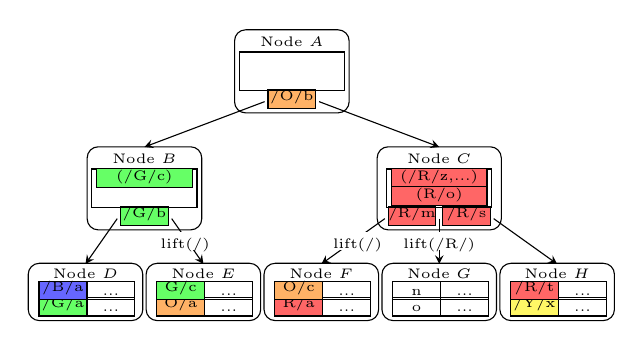
\begin{tikzpicture}[xscale=0.95, yscale=0.95]
            \node[anchor=south, rectangle, rounded corners, minimum height=.06\textwidth, minimum width=.12\textwidth, draw=black] at (0, 0) {};
            \node[anchor=south, font=\tiny] at (0, .036\textwidth) {Node $F$};
            \node[anchor=south, rectangle, minimum height=.015\textwidth, minimum width=.05\textwidth, draw=black, fill={red!60}] at (-.025\textwidth, .005\textwidth) {};
            \node[anchor=south, font=\tiny] at (-.025\textwidth, 0) {R/a};
            \node[anchor=south, rectangle, minimum height=.015\textwidth, minimum width=.05\textwidth, draw=black] at (.028\textwidth, .005\textwidth) {};
            \node[anchor=south, font=\tiny] at (.028\textwidth, 0) {...};
            \node[anchor=south, rectangle, minimum height=.015\textwidth, minimum width=.05\textwidth, draw=black, fill={orange!60}] at (-.025\textwidth, .023\textwidth) {};
            \node[anchor=south, font=\tiny] at (-.025\textwidth, .018\textwidth) {O/c};
            \node[anchor=south, rectangle, minimum height=.015\textwidth, minimum width=.05\textwidth, draw=black] at (.028\textwidth, .023\textwidth) {};
            \node[anchor=south, font=\tiny] at (.028\textwidth, .018\textwidth) {...};

            \node[anchor=south, rectangle, rounded corners, minimum height=.06\textwidth, minimum width=.12\textwidth, draw=black] at (.13\textwidth, 0) {};
            \node[anchor=south, font=\tiny] at (.13\textwidth, .036\textwidth) {Node $G$};
            \node[anchor=south, rectangle, minimum height=.015\textwidth, minimum width=.05\textwidth, draw=black] at (.105\textwidth, .005\textwidth) {};
            \node[anchor=south, font=\tiny] at (.105\textwidth, 0) {o};
            \node[anchor=south, rectangle, minimum height=.015\textwidth, minimum width=.05\textwidth, draw=black] at (.158\textwidth, .005\textwidth) {};
            \node[anchor=south, font=\tiny] at (.158\textwidth, 0) {...};
            \node[anchor=south, rectangle, minimum height=.015\textwidth, minimum width=.05\textwidth, draw=black] at (.105\textwidth, .023\textwidth) {};
            \node[anchor=south, font=\tiny] at (.105\textwidth, .018\textwidth) {n};
            \node[anchor=south, rectangle, minimum height=.015\textwidth, minimum width=.05\textwidth, draw=black] at (.158\textwidth, .023\textwidth) {};
            \node[anchor=south, font=\tiny] at (.158\textwidth, .018\textwidth) {...};

            \node[anchor=south, rectangle, rounded corners, minimum height=.06\textwidth, minimum width=.12\textwidth, draw=black] at (.26\textwidth, 0) {};
            \node[anchor=south, font=\tiny] at (.26\textwidth, .036\textwidth) {Node $H$};
            \node[anchor=south, rectangle, minimum height=.015\textwidth, minimum width=.05\textwidth, draw=black, fill={yellow!60}] at (.235\textwidth, .005\textwidth) {};
            \node[anchor=south, font=\tiny] at (.235\textwidth, 0) {/Y/x};
            \node[anchor=south, rectangle, minimum height=.015\textwidth, minimum width=.05\textwidth, draw=black] at (.288\textwidth, .005\textwidth) {};
            \node[anchor=south, font=\tiny] at (.288\textwidth, 0) {...};
            \node[anchor=south, rectangle, minimum height=.015\textwidth, minimum width=.05\textwidth, draw=black, fill={red!60}] at (.235\textwidth, .023\textwidth) {};
            \node[anchor=south, font=\tiny] at (.235\textwidth, .018\textwidth) {/R/t};
            \node[anchor=south, rectangle, minimum height=.015\textwidth, minimum width=.05\textwidth, draw=black] at (.288\textwidth, .023\textwidth) {};
            \node[anchor=south, font=\tiny] at (.288\textwidth, .018\textwidth) {...};

            \node[anchor=south, rectangle, rounded corners, minimum height=.06\textwidth, minimum width=.12\textwidth, draw=black] at (-.13\textwidth, 0) {};
            \node[anchor=south, font=\tiny] at (-.13\textwidth, .036\textwidth) {Node $E$};
            \node[anchor=south, rectangle, minimum height=.015\textwidth, minimum width=.05\textwidth, draw=black, fill={orange!60}] at (-.155\textwidth, .005\textwidth) {};
            \node[anchor=south, font=\tiny] at (-.155\textwidth, 0) {O/a};
            \node[anchor=south, rectangle, minimum height=.015\textwidth, minimum width=.05\textwidth, draw=black] at (-.102\textwidth, .005\textwidth) {};
            \node[anchor=south, font=\tiny] at (-.102\textwidth, 0) {...};
            \node[anchor=south, rectangle, minimum height=.015\textwidth, minimum width=.05\textwidth, draw=black, fill={green!60}] at (-.155\textwidth, .023\textwidth) {};
            \node[anchor=south, font=\tiny] at (-.155\textwidth, .018\textwidth) {G/c};
            \node[anchor=south, rectangle, minimum height=.015\textwidth, minimum width=.05\textwidth, draw=black] at (-.102\textwidth, .023\textwidth) {};
            \node[anchor=south, font=\tiny] at (-.102\textwidth, .018\textwidth) {...};

            \node[anchor=south, rectangle, rounded corners, minimum height=.06\textwidth, minimum width=.12\textwidth, draw=black] at (-.26\textwidth, 0) {};
            \node[anchor=south, font=\tiny] at (-.26\textwidth, .036\textwidth) {Node $D$};
            \node[anchor=south, rectangle, minimum height=.015\textwidth, minimum width=.05\textwidth, draw=black, fill={green!60}] at (-.285\textwidth, .005\textwidth) {};
            \node[anchor=south, font=\tiny] at (-.285\textwidth, 0) {/G/a};
            \node[anchor=south, rectangle, minimum height=.015\textwidth, minimum width=.05\textwidth, draw=black] at (-.232\textwidth, .005\textwidth) {};
            \node[anchor=south, font=\tiny] at (-.232\textwidth, 0) {...};
            \node[anchor=south, rectangle, minimum height=.015\textwidth, minimum width=.05\textwidth, draw=black, fill={blue!60}] at (-.285\textwidth, .023\textwidth) {};
            \node[anchor=south, font=\tiny] at (-.285\textwidth, .018\textwidth) {/B/a};
            \node[anchor=south, rectangle, minimum height=.015\textwidth, minimum width=.05\textwidth, draw=black] at (-.232\textwidth, .023\textwidth) {};
            \node[anchor=south, font=\tiny] at (-.232\textwidth, .018\textwidth) {...};

            \node[anchor=south, rectangle, rounded corners, minimum height=.087\textwidth, minimum width=.12\textwidth, draw=black] at (-.195\textwidth, .1\textwidth) {};
            \node[anchor=south, font=\tiny] at (-.195\textwidth, .163\textwidth) {Node $B$};
            \node[anchor=south, rectangle, minimum height=.015\textwidth, minimum width=.05\textwidth, draw=black, fill={green!60}] at (-.195\textwidth, .105\textwidth) {};
            \node[anchor=south, font=\tiny] at (-.195\textwidth, .1\textwidth) {/G/b};
            \node[anchor=south, rectangle, minimum height=.04\textwidth, minimum width=.11\textwidth, draw=black] at (-.195\textwidth, .125\textwidth) {};
            \node[anchor=south, rectangle, minimum height=.015\textwidth, minimum width=.1\textwidth, draw=black, fill={green!60}] at (-.195\textwidth, .147\textwidth) {};
            \node[anchor=south, font=\tiny] at  (-.195\textwidth, .141\textwidth) {\delm(/G/c)};

            \node[anchor=south, rectangle, rounded corners, minimum height=.087\textwidth, minimum width=.13\textwidth, draw=black] at (.13\textwidth, .1\textwidth) {};
            \node[anchor=south, font=\tiny] at (.13\textwidth, .163\textwidth) {Node $C$};
            \node[anchor=south, rectangle, minimum height=.015\textwidth, minimum width=.05\textwidth, draw=black, fill={red!60}] at (.1\textwidth, .105\textwidth) {};
            \node[anchor=south, font=\tiny] at (.1\textwidth, .1\textwidth) {/R/m};
            \node[anchor=south, rectangle, minimum height=.015\textwidth, minimum width=.05\textwidth, draw=black, fill={red!60}] at (.16\textwidth, .105\textwidth) {};
            \node[anchor=south, font=\tiny] at (.16\textwidth, .1\textwidth) {/R/s};
            \node[anchor=south, rectangle, minimum height=.04\textwidth, minimum width=.11\textwidth, draw=black] at (.13\textwidth, .125\textwidth) {};
            \node[anchor=south, rectangle, minimum height=.015\textwidth, minimum width=.1\textwidth, draw=black, fill={red!60}] at (.13\textwidth, .147\textwidth) {};
            \node[anchor=south, font=\tiny] at  (.13\textwidth, .141\textwidth) {\putm(/R/z,...)};
            \node[anchor=south, rectangle, minimum height=.015\textwidth, minimum width=.1\textwidth, draw=black, fill={red!60}] at (.13\textwidth, .127\textwidth) {};
            \node[anchor=south, font=\tiny] at  (.13\textwidth, .121\textwidth) {\delm(R/o)};

            \node[anchor=south, rectangle, rounded corners, minimum height=.087\textwidth, minimum width=.12\textwidth, draw=black] at (-.0325\textwidth, .229\textwidth) {};
            \node[anchor=south, font=\tiny] at (-.0325\textwidth, .292\textwidth) {Node $A$};
            \node[anchor=south, rectangle, minimum height=.015\textwidth, minimum width=.05\textwidth, draw=black, fill={orange!60}] at (-.0325\textwidth, .234\textwidth) {};
            \node[anchor=south, font=\tiny] at (-.0325\textwidth, .229\textwidth) {/O/b};
            \node[anchor=south, rectangle, minimum height=.04\textwidth, minimum width=.11\textwidth, draw=black] at (-.0325\textwidth, .254\textwidth) {};

            \draw[->, >=stealth] (-.225\textwidth, .113\textwidth) -- (-.26\textwidth, .063\textwidth);
            \draw[->, >=stealth] (-.165\textwidth, .113\textwidth) -- (-.13\textwidth, .063\textwidth);
            \draw[->, >=stealth] (.13\textwidth, .113\textwidth) -- (.13\textwidth, .063\textwidth);
            \draw[->, >=stealth] (.19\textwidth, .113\textwidth) -- (.26\textwidth, .063\textwidth);
            \draw[->, >=stealth] (.07\textwidth, .113\textwidth) -- (0, .063\textwidth);
            \draw[->, >=stealth] (-.0625\textwidth, .242\textwidth) -- (-.195\textwidth, .192\textwidth);
            \draw[->, >=stealth] (-.0025\textwidth, .242\textwidth) -- (.13\textwidth, .192\textwidth);

            \node[anchor=north,rectangle, minimum height=.015\textwidth, minimum width=.05\textwidth, fill={white}] at (.13\textwidth, .099\textwidth) {};
            \node[anchor=north, font=\tiny] at (.13\textwidth, .102\textwidth) {lift(/R/)};
            \node[anchor=north,rectangle, minimum height=.015\textwidth, minimum width=.05\textwidth, fill={white}] at (.04\textwidth, .099\textwidth) {};
            \node[anchor=north, font=\tiny] at (.04\textwidth, .102\textwidth) {lift(/)};
            \node[anchor=north,rectangle, minimum height=.015\textwidth, minimum width=.05\textwidth, fill={white}] at (-.15\textwidth, .099\textwidth) {};
            \node[anchor=north, font=\tiny] at (-.15\textwidth, .102\textwidth) {lift(/)};
        \end{tikzpicture}
        \caption{\label{subfig:goto-2}
            The range-clone operation reaches the source LCA, Node $C$,
            flushing messages along the way.}
    \end{subfigure}
    \begin{subfigure}{\textwidth}
        \centering
        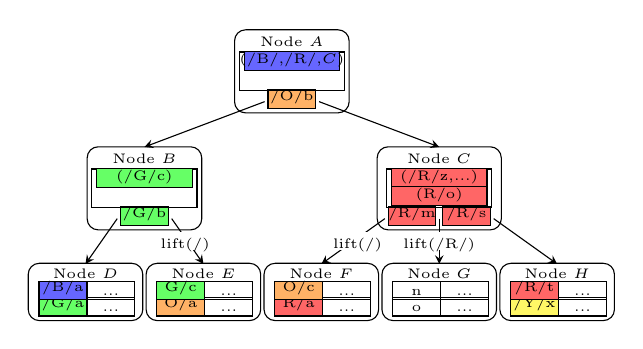
\begin{tikzpicture}[xscale=0.95, yscale=0.95]
            \node[anchor=south, rectangle, rounded corners, minimum height=.06\textwidth, minimum width=.12\textwidth, draw=black] at (0, 0) {};
            \node[anchor=south, font=\tiny] at (0, .036\textwidth) {Node $F$};
            \node[anchor=south, rectangle, minimum height=.015\textwidth, minimum width=.05\textwidth, draw=black, fill={red!60}] at (-.025\textwidth, .005\textwidth) {};
            \node[anchor=south, font=\tiny] at (-.025\textwidth, 0) {R/a};
            \node[anchor=south, rectangle, minimum height=.015\textwidth, minimum width=.05\textwidth, draw=black] at (.028\textwidth, .005\textwidth) {};
            \node[anchor=south, font=\tiny] at (.028\textwidth, 0) {...};
            \node[anchor=south, rectangle, minimum height=.015\textwidth, minimum width=.05\textwidth, draw=black, fill={orange!60}] at (-.025\textwidth, .023\textwidth) {};
            \node[anchor=south, font=\tiny] at (-.025\textwidth, .018\textwidth) {O/c};
            \node[anchor=south, rectangle, minimum height=.015\textwidth, minimum width=.05\textwidth, draw=black] at (.028\textwidth, .023\textwidth) {};
            \node[anchor=south, font=\tiny] at (.028\textwidth, .018\textwidth) {...};

            \node[anchor=south, rectangle, rounded corners, minimum height=.06\textwidth, minimum width=.12\textwidth, draw=black] at (.13\textwidth, 0) {};
            \node[anchor=south, font=\tiny] at (.13\textwidth, .036\textwidth) {Node $G$};
            \node[anchor=south, rectangle, minimum height=.015\textwidth, minimum width=.05\textwidth, draw=black] at (.105\textwidth, .005\textwidth) {};
            \node[anchor=south, font=\tiny] at (.105\textwidth, 0) {o};
            \node[anchor=south, rectangle, minimum height=.015\textwidth, minimum width=.05\textwidth, draw=black] at (.158\textwidth, .005\textwidth) {};
            \node[anchor=south, font=\tiny] at (.158\textwidth, 0) {...};
            \node[anchor=south, rectangle, minimum height=.015\textwidth, minimum width=.05\textwidth, draw=black] at (.105\textwidth, .023\textwidth) {};
            \node[anchor=south, font=\tiny] at (.105\textwidth, .018\textwidth) {n};
            \node[anchor=south, rectangle, minimum height=.015\textwidth, minimum width=.05\textwidth, draw=black] at (.158\textwidth, .023\textwidth) {};
            \node[anchor=south, font=\tiny] at (.158\textwidth, .018\textwidth) {...};

            \node[anchor=south, rectangle, rounded corners, minimum height=.06\textwidth, minimum width=.12\textwidth, draw=black] at (.26\textwidth, 0) {};
            \node[anchor=south, font=\tiny] at (.26\textwidth, .036\textwidth) {Node $H$};
            \node[anchor=south, rectangle, minimum height=.015\textwidth, minimum width=.05\textwidth, draw=black, fill={yellow!60}] at (.235\textwidth, .005\textwidth) {};
            \node[anchor=south, font=\tiny] at (.235\textwidth, 0) {/Y/x};
            \node[anchor=south, rectangle, minimum height=.015\textwidth, minimum width=.05\textwidth, draw=black] at (.288\textwidth, .005\textwidth) {};
            \node[anchor=south, font=\tiny] at (.288\textwidth, 0) {...};
            \node[anchor=south, rectangle, minimum height=.015\textwidth, minimum width=.05\textwidth, draw=black, fill={red!60}] at (.235\textwidth, .023\textwidth) {};
            \node[anchor=south, font=\tiny] at (.235\textwidth, .018\textwidth) {/R/t};
            \node[anchor=south, rectangle, minimum height=.015\textwidth, minimum width=.05\textwidth, draw=black] at (.288\textwidth, .023\textwidth) {};
            \node[anchor=south, font=\tiny] at (.288\textwidth, .018\textwidth) {...};

            \node[anchor=south, rectangle, rounded corners, minimum height=.06\textwidth, minimum width=.12\textwidth, draw=black] at (-.13\textwidth, 0) {};
            \node[anchor=south, font=\tiny] at (-.13\textwidth, .036\textwidth) {Node $E$};
            \node[anchor=south, rectangle, minimum height=.015\textwidth, minimum width=.05\textwidth, draw=black, fill={orange!60}] at (-.155\textwidth, .005\textwidth) {};
            \node[anchor=south, font=\tiny] at (-.155\textwidth, 0) {O/a};
            \node[anchor=south, rectangle, minimum height=.015\textwidth, minimum width=.05\textwidth, draw=black] at (-.102\textwidth, .005\textwidth) {};
            \node[anchor=south, font=\tiny] at (-.102\textwidth, 0) {...};
            \node[anchor=south, rectangle, minimum height=.015\textwidth, minimum width=.05\textwidth, draw=black, fill={green!60}] at (-.155\textwidth, .023\textwidth) {};
            \node[anchor=south, font=\tiny] at (-.155\textwidth, .018\textwidth) {G/c};
            \node[anchor=south, rectangle, minimum height=.015\textwidth, minimum width=.05\textwidth, draw=black] at (-.102\textwidth, .023\textwidth) {};
            \node[anchor=south, font=\tiny] at (-.102\textwidth, .018\textwidth) {...};

            \node[anchor=south, rectangle, rounded corners, minimum height=.06\textwidth, minimum width=.12\textwidth, draw=black] at (-.26\textwidth, 0) {};
            \node[anchor=south, font=\tiny] at (-.26\textwidth, .036\textwidth) {Node $D$};
            \node[anchor=south, rectangle, minimum height=.015\textwidth, minimum width=.05\textwidth, draw=black, fill={green!60}] at (-.285\textwidth, .005\textwidth) {};
            \node[anchor=south, font=\tiny] at (-.285\textwidth, 0) {/G/a};
            \node[anchor=south, rectangle, minimum height=.015\textwidth, minimum width=.05\textwidth, draw=black] at (-.232\textwidth, .005\textwidth) {};
            \node[anchor=south, font=\tiny] at (-.232\textwidth, 0) {...};
            \node[anchor=south, rectangle, minimum height=.015\textwidth, minimum width=.05\textwidth, draw=black, fill={blue!60}] at (-.285\textwidth, .023\textwidth) {};
            \node[anchor=south, font=\tiny] at (-.285\textwidth, .018\textwidth) {/B/a};
            \node[anchor=south, rectangle, minimum height=.015\textwidth, minimum width=.05\textwidth, draw=black] at (-.232\textwidth, .023\textwidth) {};
            \node[anchor=south, font=\tiny] at (-.232\textwidth, .018\textwidth) {...};

            \node[anchor=south, rectangle, rounded corners, minimum height=.087\textwidth, minimum width=.12\textwidth, draw=black] at (-.195\textwidth, .1\textwidth) {};
            \node[anchor=south, font=\tiny] at (-.195\textwidth, .163\textwidth) {Node $B$};
            \node[anchor=south, rectangle, minimum height=.015\textwidth, minimum width=.05\textwidth, draw=black, fill={green!60}] at (-.195\textwidth, .105\textwidth) {};
            \node[anchor=south, font=\tiny] at (-.195\textwidth, .1\textwidth) {/G/b};
            \node[anchor=south, rectangle, minimum height=.04\textwidth, minimum width=.11\textwidth, draw=black] at (-.195\textwidth, .125\textwidth) {};
            \node[anchor=south, rectangle, minimum height=.015\textwidth, minimum width=.1\textwidth, draw=black, fill={green!60}] at (-.195\textwidth, .147\textwidth) {};
            \node[anchor=south, font=\tiny] at  (-.195\textwidth, .141\textwidth) {\delm(/G/c)};

            \node[anchor=south, rectangle, rounded corners, minimum height=.087\textwidth, minimum width=.13\textwidth, draw=black] at (.13\textwidth, .1\textwidth) {};
            \node[anchor=south, font=\tiny] at (.13\textwidth, .163\textwidth) {Node $C$};
            \node[anchor=south, rectangle, minimum height=.015\textwidth, minimum width=.05\textwidth, draw=black, fill={red!60}] at (.1\textwidth, .105\textwidth) {};
            \node[anchor=south, font=\tiny] at (.1\textwidth, .1\textwidth) {/R/m};
            \node[anchor=south, rectangle, minimum height=.015\textwidth, minimum width=.05\textwidth, draw=black, fill={red!60}] at (.16\textwidth, .105\textwidth) {};
            \node[anchor=south, font=\tiny] at (.16\textwidth, .1\textwidth) {/R/s};
            \node[anchor=south, rectangle, minimum height=.04\textwidth, minimum width=.11\textwidth, draw=black] at (.13\textwidth, .125\textwidth) {};
            \node[anchor=south, rectangle, minimum height=.015\textwidth, minimum width=.1\textwidth, draw=black, fill={red!60}] at (.13\textwidth, .147\textwidth) {};
            \node[anchor=south, font=\tiny] at  (.13\textwidth, .141\textwidth) {\putm(/R/z,...)};
            \node[anchor=south, rectangle, minimum height=.015\textwidth, minimum width=.1\textwidth, draw=black, fill={red!60}] at (.13\textwidth, .127\textwidth) {};
            \node[anchor=south, font=\tiny] at  (.13\textwidth, .121\textwidth) {\delm(R/o)};

            \node[anchor=south, rectangle, rounded corners, minimum height=.087\textwidth, minimum width=.12\textwidth, draw=black] at (-.0325\textwidth, .229\textwidth) {};
            \node[anchor=south, font=\tiny] at (-.0325\textwidth, .292\textwidth) {Node $A$};
            \node[anchor=south, rectangle, minimum height=.015\textwidth, minimum width=.05\textwidth, draw=black, fill={orange!60}] at (-.0325\textwidth, .234\textwidth) {};
            \node[anchor=south, font=\tiny] at (-.0325\textwidth, .229\textwidth) {/O/b};
            \node[anchor=south, rectangle, minimum height=.04\textwidth, minimum width=.11\textwidth, draw=black] at (-.0325\textwidth, .254\textwidth) {};
            \node[anchor=south, rectangle, minimum height=.015\textwidth, minimum width=.1\textwidth, draw=black, fill={blue!60}] at (-.0325\textwidth, .276\textwidth) {};
            \node[anchor=south, font=\tiny] at  (-.0325\textwidth, .27\textwidth) {\goto(/B/,/R/,$C$)};

            \draw[->, >=stealth] (-.225\textwidth, .113\textwidth) -- (-.26\textwidth, .063\textwidth);
            \draw[->, >=stealth] (-.165\textwidth, .113\textwidth) -- (-.13\textwidth, .063\textwidth);
            \draw[->, >=stealth] (.13\textwidth, .113\textwidth) -- (.13\textwidth, .063\textwidth);
            \draw[->, >=stealth] (.19\textwidth, .113\textwidth) -- (.26\textwidth, .063\textwidth);
            \draw[->, >=stealth] (.07\textwidth, .113\textwidth) -- (0, .063\textwidth);
            \draw[->, >=stealth] (-.0625\textwidth, .242\textwidth) -- (-.195\textwidth, .192\textwidth);
            \draw[->, >=stealth] (-.0025\textwidth, .242\textwidth) -- (.13\textwidth, .192\textwidth);

            \node[anchor=north,rectangle, minimum height=.015\textwidth, minimum width=.05\textwidth, fill={white}] at (.13\textwidth, .099\textwidth) {};
            \node[anchor=north, font=\tiny] at (.13\textwidth, .102\textwidth) {lift(/R/)};
            \node[anchor=north,rectangle, minimum height=.015\textwidth, minimum width=.05\textwidth, fill={white}] at (.04\textwidth, .099\textwidth) {};
            \node[anchor=north, font=\tiny] at (.04\textwidth, .102\textwidth) {lift(/)};
            \node[anchor=north,rectangle, minimum height=.015\textwidth, minimum width=.05\textwidth, fill={white}] at (-.15\textwidth, .099\textwidth) {};
            \node[anchor=north, font=\tiny] at (-.15\textwidth, .102\textwidth) {lift(/)};
        \end{tikzpicture}
        \caption{\label{subfig:goto-3} The range-clone operation injects a \goto message
            for destination (``/B/'') keys into the root node.}
    \end{subfigure}
    \caption[A range-clone example with a \goto message]{\label{fig:goto}
        An example of completing range-clone(``/R/'', ``/B/'') with a \goto message.}
\end{figure}

For example, in Figure~\ref{subfig:goto-3}, consider a query for key ``/B/a''.
The query first visits the root node, Node $A$, and finds a \goto message,
\goto(``/B/'', ``/R'', $C$).
This query should follow the \goto message and visit Node $C$,
instead of the normal parent-to-child pointer to Node $B$.
Additionally, the \goto message acts as an \xf function that translates the
search key from ``/B/a'' to ``/R/a'' and bounds the query result to
(``/R/$_{min}$'', ``/R/$_{max}$'').
After fetching the key/value pair with key ``/R/a'' in Node $F$,
the query reconstructs the key by replacing prefix ``/R/'' with prefix ``/B/''.
Therefore, the query returns the key/value pair with key ``/B/a''.
To see why the \goto message needs to bound the query result,
consider a range query for a key that is greater than ``/B/z''.
The \goto message in Node $A$ translates the search key to ``/R/z''.
However, searching for a key greater than ``/R/z'' in the subtree rooted at
Node $C$ returns key ``/Y/x'',
which the query cannot reconstruct by replacing prefix ``/R/'' with prefix
``/B/''.
In fact, the \goto message is only for results whose keys fall in the key
range (``/B/$_{min}$'', ``/B/$_{max}$''),
therefore, any key that is not in the key range
(``/R/$_{min}$'', ``/R/$_{max}$'') is invalid after following the \goto message.

Because a \goto message redirects queries whose search keys have a certain
prefix, it also acts as a range-delete message that invalidates all old messages
and key/value pairs following other pointers (normal parent-to-child pointers
and older \goto messages).
Thus, if we set the node ID in a \goto message to a special value
(for example, 0), the \goto message acts as a range-delete message.
Therefore, we can use \goto messages to implement range-delete.

Though a \goto message acts as an additional parent-to-child pointer in the node,
the child of the \goto message doesn't need to be at the same height as
normal children of the node.
Therefore, the \goto message let us share a subtree between two parents
at different heights.

Also, the \xf function associated with the \goto message means the target
subtree can have a larger key range than specified in the \goto message.
Thus, the range-clone operation can lazily slice out the subtrees,
amortizing the slicing cost with other operations.

\paragraph{Range-clone with \goto messages.}

Range-clone(\spre, \dpre) is implemented with \goto messages through the
following steps:
\begin{itemize}
\item the range-clone operation does a root-to-leaf traversal with \spre
until reaching the source LCA, the lowest node that covers the whole key range
(\spre$_{min}$, \spre$_{max}$).
During the traversal, the range-clone operation also flushes messages from
parent to child.
At this point, all messages with keys in the cloned key range
are in the subtree rooted at the source LCA.
\item the range-clone message then injects a \goto message into the root node of
the lifted \bedag with the source LCA as the node ID in the \goto message,
increasing the reference count of the source LCA by 1.
\end{itemize}
Briefly speaking, on the critical path, the range-clone operation flushes
messages until the source LCA, increments the reference count of the source LCA,
and injects a \goto message into the root node.
Note, this range-clone operation doesn't do tree surgery or pointer swings
on the critical path.

Figure~\ref{fig:goto} shows an example of range-clone(``/R/'', ``/B/'')
that generates a \goto message.
Figure~\ref{subfig:goto-1} shows the \bet before the range-clone operation.
Starting from the root node, Node $A$, the range-clone operation traverses to
the source LCA, Node $C$.
At the same time, it flushes the message, \delm(``/R/z''), to Node $C$.
Figure~\ref{subfig:goto-2} shows the \bet after the range-clone operation
reaches the source LCA.
Finally, the range-clone operation injects a \goto message into the root node,
with ``/B/'' as its \dpre, ``/R/'' as its \spre and Node $C$ as its node ID.
Figure~\ref{subfig:goto-3} shows the result.
Now, consider a query for key ``/B/a''.
The query starts at the Node $A$.
Then, instead of following the parent-to-child pointers to Node $B$, it follows
the \goto message and visits Node $C$.
The \goto message also acts as an \xf function that translates the search key
to ``/R/a'' and bounds the result in range (``/R/$_{min}$'', ``/R/$_{max}$'').
At last, the query finds the correct key/value pair in Node $F$.

\subsection{Flushing \goto messages}
\label{sec:rc:flush}

A \goto message prevents the \bet from flushing future messages that
fall in the key range of the \goto message,
because queries will not follow the normal parent-to-child pointer and find
the messages once flushed.
Therefore, the lifted \bedag should flush \goto messages along with other messages.

However, flushing a \goto message to a node at the same height as the source
LCA breaks the asymptotic I/O costs of queries in the lifted \bedag,
because such a \goto message redirects queries to a node at the same height.
Therefore, when flushing a \goto message to a node at the same height as
the source LCA,
the lifted \bedag transfers the \goto message to
pivots and a parent-to-child pointer.

This subsection explains how the lifted \bedag flushes \goto messages.
We start from the simple case, where a \goto message is being flushed to nodes
higher than the source LCA.
Then, we describe how a \goto message becomes pivots and a parent-to-child
pointer
when the lifted \bedag flushes the \goto message to
a node at the same height as the source LCA.

\paragraph{The lifted \bedag flushes a \goto message to a node higher than
the source LCA.}
In the simple case, the node that tries to flush a \goto message has a single
child that covers the key range of the \goto message
and the child is higher than the source LCA of the \goto message.
Flushing the \goto message simply lifts the \dpre of the \goto message and moves
the \goto message from the node's buffer to the child's buffer.

\begin{figure}
    \begin{subfigure}{\textwidth}
        \centering
        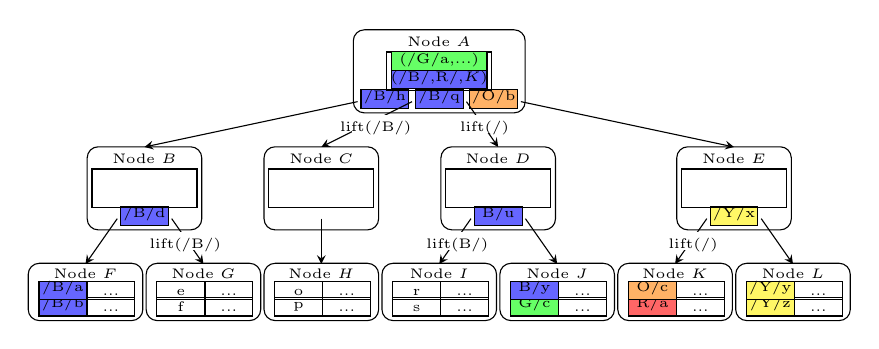
\begin{tikzpicture}[xscale=0.95, yscale=0.95]
            \node[anchor=south, rectangle, rounded corners, minimum height=.06\textwidth, minimum width=.12\textwidth, draw=black] at (0, 0) {};
            \node[anchor=south, font=\tiny] at (0, .036\textwidth) {Node $F$};
            \node[anchor=south, rectangle, minimum height=.015\textwidth, minimum width=.05\textwidth, draw=black, fill={blue!60}] at (-.025\textwidth, .005\textwidth) {};
            \node[anchor=south, font=\tiny] at (-.025\textwidth, 0) {/B/b};
            \node[anchor=south, rectangle, minimum height=.015\textwidth, minimum width=.05\textwidth, draw=black] at (.028\textwidth, .005\textwidth) {};
            \node[anchor=south, font=\tiny] at (.028\textwidth, 0) {...};
            \node[anchor=south, rectangle, minimum height=.015\textwidth, minimum width=.05\textwidth, draw=black, fill={blue!60}] at (-.025\textwidth, .023\textwidth) {};
            \node[anchor=south, font=\tiny] at (-.025\textwidth, .018\textwidth) {/B/a};
            \node[anchor=south, rectangle, minimum height=.015\textwidth, minimum width=.05\textwidth, draw=black] at (.028\textwidth, .023\textwidth) {};
            \node[anchor=south, font=\tiny] at (.028\textwidth, .018\textwidth) {...};

            \node[anchor=south, rectangle, rounded corners, minimum height=.06\textwidth, minimum width=.12\textwidth, draw=black] at (.13\textwidth, 0) {};
            \node[anchor=south, font=\tiny] at (.13\textwidth, .036\textwidth) {Node $G$};
            \node[anchor=south, rectangle, minimum height=.015\textwidth, minimum width=.05\textwidth, draw=black] at (.105\textwidth, .005\textwidth) {};
            \node[anchor=south, font=\tiny] at (.105\textwidth, 0) {f};
            \node[anchor=south, rectangle, minimum height=.015\textwidth, minimum width=.05\textwidth, draw=black] at (.158\textwidth, .005\textwidth) {};
            \node[anchor=south, font=\tiny] at (.158\textwidth, 0) {...};
            \node[anchor=south, rectangle, minimum height=.015\textwidth, minimum width=.05\textwidth, draw=black] at (.105\textwidth, .023\textwidth) {};
            \node[anchor=south, font=\tiny] at (.105\textwidth, .018\textwidth) {e};
            \node[anchor=south, rectangle, minimum height=.015\textwidth, minimum width=.05\textwidth, draw=black] at (.158\textwidth, .023\textwidth) {};
            \node[anchor=south, font=\tiny] at (.158\textwidth, .018\textwidth) {...};

            \node[anchor=south, rectangle, rounded corners, minimum height=.06\textwidth, minimum width=.12\textwidth, draw=black] at (.26\textwidth, 0) {};
            \node[anchor=south, font=\tiny] at (.26\textwidth, .036\textwidth) {Node $H$};
            \node[anchor=south, rectangle, minimum height=.015\textwidth, minimum width=.05\textwidth, draw=black] at (.235\textwidth, .005\textwidth) {};
            \node[anchor=south, font=\tiny] at (.235\textwidth, 0) {p};
            \node[anchor=south, rectangle, minimum height=.015\textwidth, minimum width=.05\textwidth, draw=black] at (.288\textwidth, .005\textwidth) {};
            \node[anchor=south, font=\tiny] at (.288\textwidth, 0) {...};
            \node[anchor=south, rectangle, minimum height=.015\textwidth, minimum width=.05\textwidth, draw=black] at (.235\textwidth, .023\textwidth) {};
            \node[anchor=south, font=\tiny] at (.235\textwidth, .018\textwidth) {o};
            \node[anchor=south, rectangle, minimum height=.015\textwidth, minimum width=.05\textwidth, draw=black] at (.288\textwidth, .023\textwidth) {};
            \node[anchor=south, font=\tiny] at (.288\textwidth, .018\textwidth) {...};

            \node[anchor=south, rectangle, rounded corners, minimum height=.06\textwidth, minimum width=.12\textwidth, draw=black] at (.39\textwidth, 0) {};
            \node[anchor=south, font=\tiny] at (.39\textwidth, .036\textwidth) {Node $I$};
            \node[anchor=south, rectangle, minimum height=.015\textwidth, minimum width=.05\textwidth, draw=black] at (.365\textwidth, .005\textwidth) {};
            \node[anchor=south, font=\tiny] at (.365\textwidth, 0) {s};
            \node[anchor=south, rectangle, minimum height=.015\textwidth, minimum width=.05\textwidth, draw=black] at (.418\textwidth, .005\textwidth) {};
            \node[anchor=south, font=\tiny] at (.418\textwidth, 0) {...};
            \node[anchor=south, rectangle, minimum height=.015\textwidth, minimum width=.05\textwidth, draw=black] at (.365\textwidth, .023\textwidth) {};
            \node[anchor=south, font=\tiny] at (.365\textwidth, .018\textwidth) {r};
            \node[anchor=south, rectangle, minimum height=.015\textwidth, minimum width=.05\textwidth, draw=black] at (.418\textwidth, .023\textwidth) {};
            \node[anchor=south, font=\tiny] at (.418\textwidth, .018\textwidth) {...};

            \node[anchor=south, rectangle, rounded corners, minimum height=.06\textwidth, minimum width=.12\textwidth, draw=black] at (.52\textwidth, 0) {};
            \node[anchor=south, font=\tiny] at (.52\textwidth, .036\textwidth) {Node $J$};
            \node[anchor=south, rectangle, minimum height=.015\textwidth, minimum width=.05\textwidth, draw=black, fill={green!60}] at (.495\textwidth, .005\textwidth) {};
            \node[anchor=south, font=\tiny] at (.495\textwidth, 0) {G/c};
            \node[anchor=south, rectangle, minimum height=.015\textwidth, minimum width=.05\textwidth, draw=black] at (.548\textwidth, .005\textwidth) {};
            \node[anchor=south, font=\tiny] at (.548\textwidth, 0) {...};
            \node[anchor=south, rectangle, minimum height=.015\textwidth, minimum width=.05\textwidth, draw=black, fill={blue!60}] at (.495\textwidth, .023\textwidth) {};
            \node[anchor=south, font=\tiny] at (.495\textwidth, .018\textwidth) {B/y};
            \node[anchor=south, rectangle, minimum height=.015\textwidth, minimum width=.05\textwidth, draw=black] at (.548\textwidth, .023\textwidth) {};
            \node[anchor=south, font=\tiny] at (.548\textwidth, .018\textwidth) {...};

            \node[anchor=south, rectangle, rounded corners, minimum height=.06\textwidth, minimum width=.12\textwidth, draw=black] at (.65\textwidth, 0) {};
            \node[anchor=south, font=\tiny] at (.65\textwidth, .036\textwidth) {Node $K$};
            \node[anchor=south, rectangle, minimum height=.015\textwidth, minimum width=.05\textwidth, draw=black, fill={red!60}] at (.625\textwidth, .005\textwidth) {};
            \node[anchor=south, font=\tiny] at (.625\textwidth, 0) {R/a};
            \node[anchor=south, rectangle, minimum height=.015\textwidth, minimum width=.05\textwidth, draw=black] at (.678\textwidth, .005\textwidth) {};
            \node[anchor=south, font=\tiny] at (.678\textwidth, 0) {...};
            \node[anchor=south, rectangle, minimum height=.015\textwidth, minimum width=.05\textwidth, draw=black, fill={orange!60}] at (.625\textwidth, .023\textwidth) {};
            \node[anchor=south, font=\tiny] at (.625\textwidth, .018\textwidth) {O/c};
            \node[anchor=south, rectangle, minimum height=.015\textwidth, minimum width=.05\textwidth, draw=black] at (.678\textwidth, .023\textwidth) {};
            \node[anchor=south, font=\tiny] at (.678\textwidth, .018\textwidth) {...};

            \node[anchor=south, rectangle, rounded corners, minimum height=.06\textwidth, minimum width=.12\textwidth, draw=black] at (.78\textwidth, 0) {};
            \node[anchor=south, font=\tiny] at (.78\textwidth, .036\textwidth) {Node $L$};
            \node[anchor=south, rectangle, minimum height=.015\textwidth, minimum width=.05\textwidth, draw=black, fill={yellow!60}] at (.755\textwidth, .005\textwidth) {};
            \node[anchor=south, font=\tiny] at (.755\textwidth, 0) {/Y/z};
            \node[anchor=south, rectangle, minimum height=.015\textwidth, minimum width=.05\textwidth, draw=black] at (.808\textwidth, .005\textwidth) {};
            \node[anchor=south, font=\tiny] at (.808\textwidth, 0) {...};
            \node[anchor=south, rectangle, minimum height=.015\textwidth, minimum width=.05\textwidth, draw=black, fill={yellow!60}] at (.755\textwidth, .023\textwidth) {};
            \node[anchor=south, font=\tiny] at (.755\textwidth, .018\textwidth) {/Y/y};
            \node[anchor=south, rectangle, minimum height=.015\textwidth, minimum width=.05\textwidth, draw=black] at (.808\textwidth, .023\textwidth) {};
            \node[anchor=south, font=\tiny] at (.808\textwidth, .018\textwidth) {...};

            \node[anchor=south, rectangle, rounded corners, minimum height=.087\textwidth, minimum width=.12\textwidth, draw=black] at (.065\textwidth, .1\textwidth) {};
            \node[anchor=south, font=\tiny] at (.065\textwidth, .163\textwidth) {Node $B$};
            \node[anchor=south, rectangle, minimum height=.015\textwidth, minimum width=.05\textwidth, draw=black, fill={blue!60}] at (.065\textwidth, .105\textwidth) {};
            \node[anchor=south, font=\tiny] at (.065\textwidth, .1\textwidth) {/B/d};
            \node[anchor=south, rectangle, minimum height=.04\textwidth, minimum width=.11\textwidth, draw=black] at (.065\textwidth, .125\textwidth) {};

            \node[anchor=south, rectangle, rounded corners, minimum height=.087\textwidth, minimum width=.12\textwidth, draw=black] at (.26\textwidth, .1\textwidth) {};
            \node[anchor=south, font=\tiny] at (.26\textwidth, .163\textwidth) {Node $C$};
            \node[anchor=south, rectangle, minimum height=.04\textwidth, minimum width=.11\textwidth, draw=black] at (.26\textwidth, .125\textwidth) {};

            \node[anchor=south, rectangle, rounded corners, minimum height=.087\textwidth, minimum width=.12\textwidth, draw=black] at (.455\textwidth, .1\textwidth) {};
            \node[anchor=south, font=\tiny] at (.455\textwidth, .163\textwidth) {Node $D$};
            \node[anchor=south, rectangle, minimum height=.015\textwidth, minimum width=.05\textwidth, draw=black, fill={blue!60}] at (.455\textwidth, .105\textwidth) {};
            \node[anchor=south, font=\tiny] at (.455\textwidth, .1\textwidth) {B/u};
            \node[anchor=south, rectangle, minimum height=.04\textwidth, minimum width=.11\textwidth, draw=black] at (.455\textwidth, .125\textwidth) {};

            \node[anchor=south, rectangle, rounded corners, minimum height=.087\textwidth, minimum width=.12\textwidth, draw=black] at (.715\textwidth, .1\textwidth) {};
            \node[anchor=south, font=\tiny] at (.715\textwidth, .163\textwidth) {Node $E$};
            \node[anchor=south, rectangle, minimum height=.015\textwidth, minimum width=.05\textwidth, draw=black, fill={yellow!60}] at (.715\textwidth, .105\textwidth) {};
            \node[anchor=south, font=\tiny] at (.715\textwidth, .1\textwidth) {/Y/x};
            \node[anchor=south, rectangle, minimum height=.04\textwidth, minimum width=.11\textwidth, draw=black] at (.715\textwidth, .125\textwidth) {};

            \node[anchor=south, rectangle, rounded corners, minimum height=.087\textwidth, minimum width=.18\textwidth, draw=black] at (.39\textwidth, .229\textwidth) {};
            \node[anchor=south, font=\tiny] at (.39\textwidth, .292\textwidth) {Node $A$};
            \node[anchor=south, rectangle, minimum height=.015\textwidth, minimum width=.05\textwidth, draw=black, fill={blue!60}] at (.33\textwidth, .234\textwidth) {};
            \node[anchor=south, font=\tiny] at (.33\textwidth, .229\textwidth) {/B/h};
            \node[anchor=south, rectangle, minimum height=.015\textwidth, minimum width=.05\textwidth, draw=black, fill={blue!60}] at (.39\textwidth, .234\textwidth) {};
            \node[anchor=south, font=\tiny] at (.39\textwidth, .229\textwidth) {/B/q};
            \node[anchor=south, rectangle, minimum height=.015\textwidth, minimum width=.05\textwidth, draw=black, fill={orange!60}] at (.45\textwidth, .234\textwidth) {};
            \node[anchor=south, font=\tiny] at (.45\textwidth, .229\textwidth) {/O/b};
            \node[anchor=south, rectangle, minimum height=.04\textwidth, minimum width=.11\textwidth, draw=black] at (.39\textwidth, .254\textwidth) {};
            \node[anchor=south, rectangle, minimum height=.015\textwidth, minimum width=.1\textwidth, draw=black, fill={blue!60}] at (.39\textwidth, .256\textwidth) {};
            \node[anchor=south, font=\tiny] at  (.39\textwidth, .25\textwidth) {\goto(/B/,R/,$K$)};
            \node[anchor=south, rectangle, minimum height=.015\textwidth, minimum width=.1\textwidth, draw=black, fill={green!60}] at (.39\textwidth, .276\textwidth) {};
            \node[anchor=south, font=\tiny] at  (.39\textwidth, .27\textwidth) {\putm(/G/a,...)};

            \draw[->, >=stealth] (.035\textwidth, .113\textwidth) -- (0, .063\textwidth);
            \draw[->, >=stealth] (.095\textwidth, .113\textwidth) -- (.13\textwidth, .063\textwidth);
            \draw[->, >=stealth] (.26\textwidth, .113\textwidth) -- (.26\textwidth, .063\textwidth);
            \draw[->, >=stealth] (.425\textwidth, .113\textwidth) -- (.39\textwidth, .063\textwidth);
            \draw[->, >=stealth] (.485\textwidth, .113\textwidth) -- (.52\textwidth, .063\textwidth);
            \draw[->, >=stealth] (.685\textwidth, .113\textwidth) -- (.65\textwidth, .063\textwidth);
            \draw[->, >=stealth] (.745\textwidth, .113\textwidth) -- (.78\textwidth, .063\textwidth);
            \draw[->, >=stealth] (.3\textwidth, .242\textwidth) -- (.065\textwidth, .192\textwidth);
            \draw[->, >=stealth] (.36\textwidth, .242\textwidth) -- (.26\textwidth, .192\textwidth);
            \draw[->, >=stealth] (.42\textwidth, .242\textwidth) -- (.455\textwidth, .192\textwidth);
            \draw[->, >=stealth] (.48\textwidth, .242\textwidth) -- (.715\textwidth, .192\textwidth);

            \node[anchor=north,rectangle, minimum height=.015\textwidth, minimum width=.05\textwidth, fill={white}] at (.32\textwidth, .228\textwidth) {};
            \node[anchor=north, font=\tiny] at (.32\textwidth, .231\textwidth) {lift(/B/)};
            \node[anchor=north,rectangle, minimum height=.015\textwidth, minimum width=.05\textwidth, fill={white}] at (.44\textwidth, .228\textwidth) {};
            \node[anchor=north, font=\tiny] at (.44\textwidth, .231\textwidth) {lift(/)};
            \node[anchor=north,rectangle, minimum height=.015\textwidth, minimum width=.05\textwidth, fill={white}] at (.11\textwidth, .099\textwidth) {};
            \node[anchor=north, font=\tiny] at (.11\textwidth, .102\textwidth) {lift(/B/)};
            \node[anchor=north,rectangle, minimum height=.015\textwidth, minimum width=.05\textwidth, fill={white}] at (.41\textwidth, .099\textwidth) {};
            \node[anchor=north, font=\tiny] at (.41\textwidth, .102\textwidth) {lift(B/)};
            \node[anchor=north,rectangle, minimum height=.015\textwidth, minimum width=.05\textwidth, fill={white}] at (.67\textwidth, .099\textwidth) {};
            \node[anchor=north, font=\tiny] at (.67\textwidth, .102\textwidth) {lift(/)};
        \end{tikzpicture}
        \caption{\label{subfig:flush-1} The lifted \bedag wants to flush the
            \goto message from Node $A$, however, the \goto message doesn't
            fit into a single child.}
    \end{subfigure}
    \begin{subfigure}{\textwidth}
        \centering
        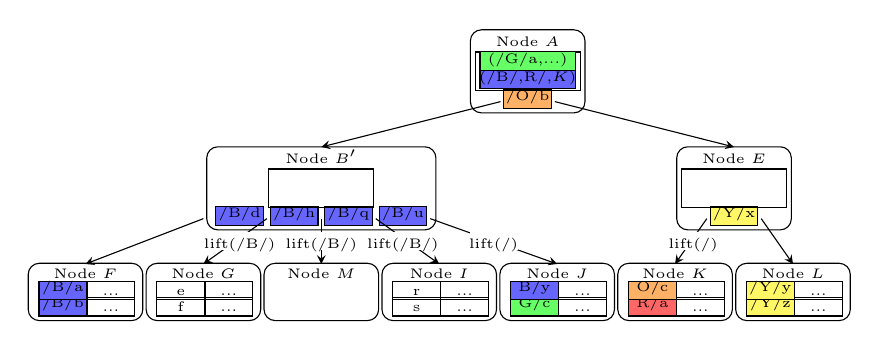
\begin{tikzpicture}[xscale=0.95, yscale=0.95]
            \node[anchor=south, rectangle, rounded corners, minimum height=.06\textwidth, minimum width=.12\textwidth, draw=black] at (0, 0) {};
            \node[anchor=south, font=\tiny] at (0, .036\textwidth) {Node $F$};
            \node[anchor=south, rectangle, minimum height=.015\textwidth, minimum width=.05\textwidth, draw=black, fill={blue!60}] at (-.025\textwidth, .005\textwidth) {};
            \node[anchor=south, font=\tiny] at (-.025\textwidth, 0) {/B/b};
            \node[anchor=south, rectangle, minimum height=.015\textwidth, minimum width=.05\textwidth, draw=black] at (.028\textwidth, .005\textwidth) {};
            \node[anchor=south, font=\tiny] at (.028\textwidth, 0) {...};
            \node[anchor=south, rectangle, minimum height=.015\textwidth, minimum width=.05\textwidth, draw=black, fill={blue!60}] at (-.025\textwidth, .023\textwidth) {};
            \node[anchor=south, font=\tiny] at (-.025\textwidth, .018\textwidth) {/B/a};
            \node[anchor=south, rectangle, minimum height=.015\textwidth, minimum width=.05\textwidth, draw=black] at (.028\textwidth, .023\textwidth) {};
            \node[anchor=south, font=\tiny] at (.028\textwidth, .018\textwidth) {...};

            \node[anchor=south, rectangle, rounded corners, minimum height=.06\textwidth, minimum width=.12\textwidth, draw=black] at (.13\textwidth, 0) {};
            \node[anchor=south, font=\tiny] at (.13\textwidth, .036\textwidth) {Node $G$};
            \node[anchor=south, rectangle, minimum height=.015\textwidth, minimum width=.05\textwidth, draw=black] at (.105\textwidth, .005\textwidth) {};
            \node[anchor=south, font=\tiny] at (.105\textwidth, 0) {f};
            \node[anchor=south, rectangle, minimum height=.015\textwidth, minimum width=.05\textwidth, draw=black] at (.158\textwidth, .005\textwidth) {};
            \node[anchor=south, font=\tiny] at (.158\textwidth, 0) {...};
            \node[anchor=south, rectangle, minimum height=.015\textwidth, minimum width=.05\textwidth, draw=black] at (.105\textwidth, .023\textwidth) {};
            \node[anchor=south, font=\tiny] at (.105\textwidth, .018\textwidth) {e};
            \node[anchor=south, rectangle, minimum height=.015\textwidth, minimum width=.05\textwidth, draw=black] at (.158\textwidth, .023\textwidth) {};
            \node[anchor=south, font=\tiny] at (.158\textwidth, .018\textwidth) {...};

            \node[anchor=south, rectangle, rounded corners, minimum height=.06\textwidth, minimum width=.12\textwidth, draw=black] at (.26\textwidth, 0) {};
            \node[anchor=south, font=\tiny] at (.26\textwidth, .036\textwidth) {Node $M$};

            \node[anchor=south, rectangle, rounded corners, minimum height=.06\textwidth, minimum width=.12\textwidth, draw=black] at (.39\textwidth, 0) {};
            \node[anchor=south, font=\tiny] at (.39\textwidth, .036\textwidth) {Node $I$};
            \node[anchor=south, rectangle, minimum height=.015\textwidth, minimum width=.05\textwidth, draw=black] at (.365\textwidth, .005\textwidth) {};
            \node[anchor=south, font=\tiny] at (.365\textwidth, 0) {s};
            \node[anchor=south, rectangle, minimum height=.015\textwidth, minimum width=.05\textwidth, draw=black] at (.418\textwidth, .005\textwidth) {};
            \node[anchor=south, font=\tiny] at (.418\textwidth, 0) {...};
            \node[anchor=south, rectangle, minimum height=.015\textwidth, minimum width=.05\textwidth, draw=black] at (.365\textwidth, .023\textwidth) {};
            \node[anchor=south, font=\tiny] at (.365\textwidth, .018\textwidth) {r};
            \node[anchor=south, rectangle, minimum height=.015\textwidth, minimum width=.05\textwidth, draw=black] at (.418\textwidth, .023\textwidth) {};
            \node[anchor=south, font=\tiny] at (.418\textwidth, .018\textwidth) {...};

            \node[anchor=south, rectangle, rounded corners, minimum height=.06\textwidth, minimum width=.12\textwidth, draw=black] at (.52\textwidth, 0) {};
            \node[anchor=south, font=\tiny] at (.52\textwidth, .036\textwidth) {Node $J$};
            \node[anchor=south, rectangle, minimum height=.015\textwidth, minimum width=.05\textwidth, draw=black, fill={green!60}] at (.495\textwidth, .005\textwidth) {};
            \node[anchor=south, font=\tiny] at (.495\textwidth, 0) {G/c};
            \node[anchor=south, rectangle, minimum height=.015\textwidth, minimum width=.05\textwidth, draw=black] at (.548\textwidth, .005\textwidth) {};
            \node[anchor=south, font=\tiny] at (.548\textwidth, 0) {...};
            \node[anchor=south, rectangle, minimum height=.015\textwidth, minimum width=.05\textwidth, draw=black, fill={blue!60}] at (.495\textwidth, .023\textwidth) {};
            \node[anchor=south, font=\tiny] at (.495\textwidth, .018\textwidth) {B/y};
            \node[anchor=south, rectangle, minimum height=.015\textwidth, minimum width=.05\textwidth, draw=black] at (.548\textwidth, .023\textwidth) {};
            \node[anchor=south, font=\tiny] at (.548\textwidth, .018\textwidth) {...};

            \node[anchor=south, rectangle, rounded corners, minimum height=.06\textwidth, minimum width=.12\textwidth, draw=black] at (.65\textwidth, 0) {};
            \node[anchor=south, font=\tiny] at (.65\textwidth, .036\textwidth) {Node $K$};
            \node[anchor=south, rectangle, minimum height=.015\textwidth, minimum width=.05\textwidth, draw=black, fill={red!60}] at (.625\textwidth, .005\textwidth) {};
            \node[anchor=south, font=\tiny] at (.625\textwidth, 0) {R/a};
            \node[anchor=south, rectangle, minimum height=.015\textwidth, minimum width=.05\textwidth, draw=black] at (.678\textwidth, .005\textwidth) {};
            \node[anchor=south, font=\tiny] at (.678\textwidth, 0) {...};
            \node[anchor=south, rectangle, minimum height=.015\textwidth, minimum width=.05\textwidth, draw=black, fill={orange!60}] at (.625\textwidth, .023\textwidth) {};
            \node[anchor=south, font=\tiny] at (.625\textwidth, .018\textwidth) {O/c};
            \node[anchor=south, rectangle, minimum height=.015\textwidth, minimum width=.05\textwidth, draw=black] at (.678\textwidth, .023\textwidth) {};
            \node[anchor=south, font=\tiny] at (.678\textwidth, .018\textwidth) {...};

            \node[anchor=south, rectangle, rounded corners, minimum height=.06\textwidth, minimum width=.12\textwidth, draw=black] at (.78\textwidth, 0) {};
            \node[anchor=south, font=\tiny] at (.78\textwidth, .036\textwidth) {Node $L$};
            \node[anchor=south, rectangle, minimum height=.015\textwidth, minimum width=.05\textwidth, draw=black, fill={yellow!60}] at (.755\textwidth, .005\textwidth) {};
            \node[anchor=south, font=\tiny] at (.755\textwidth, 0) {/Y/z};
            \node[anchor=south, rectangle, minimum height=.015\textwidth, minimum width=.05\textwidth, draw=black] at (.808\textwidth, .005\textwidth) {};
            \node[anchor=south, font=\tiny] at (.808\textwidth, 0) {...};
            \node[anchor=south, rectangle, minimum height=.015\textwidth, minimum width=.05\textwidth, draw=black, fill={yellow!60}] at (.755\textwidth, .023\textwidth) {};
            \node[anchor=south, font=\tiny] at (.755\textwidth, .018\textwidth) {/Y/y};
            \node[anchor=south, rectangle, minimum height=.015\textwidth, minimum width=.05\textwidth, draw=black] at (.808\textwidth, .023\textwidth) {};
            \node[anchor=south, font=\tiny] at (.808\textwidth, .018\textwidth) {...};

            \node[anchor=south, rectangle, rounded corners, minimum height=.087\textwidth, minimum width=.24\textwidth, draw=black] at (.26\textwidth, .1\textwidth) {};
            \node[anchor=south, font=\tiny] at (.26\textwidth, .163\textwidth) {Node $B'$};
            \node[anchor=south, rectangle, minimum height=.015\textwidth, minimum width=.05\textwidth, draw=black, fill={blue!60}] at (.17\textwidth, .105\textwidth) {};
            \node[anchor=south, font=\tiny] at (.17\textwidth, .1\textwidth) {/B/d};
            \node[anchor=south, rectangle, minimum height=.015\textwidth, minimum width=.05\textwidth, draw=black, fill={blue!60}] at (.23\textwidth, .105\textwidth) {};
            \node[anchor=south, font=\tiny] at (.23\textwidth, .1\textwidth) {/B/h};
            \node[anchor=south, rectangle, minimum height=.015\textwidth, minimum width=.05\textwidth, draw=black, fill={blue!60}] at (.29\textwidth, .105\textwidth) {};
            \node[anchor=south, font=\tiny] at (.29\textwidth, .1\textwidth) {/B/q};
            \node[anchor=south, rectangle, minimum height=.015\textwidth, minimum width=.05\textwidth, draw=black, fill={blue!60}] at (.35\textwidth, .105\textwidth) {};
            \node[anchor=south, font=\tiny] at (.35\textwidth, .1\textwidth) {/B/u};
            \node[anchor=south, rectangle, minimum height=.04\textwidth, minimum width=.11\textwidth, draw=black] at (.26\textwidth, .125\textwidth) {};

            \node[anchor=south, rectangle, rounded corners, minimum height=.087\textwidth, minimum width=.12\textwidth, draw=black] at (.715\textwidth, .1\textwidth) {};
            \node[anchor=south, font=\tiny] at (.715\textwidth, .163\textwidth) {Node $E$};
            \node[anchor=south, rectangle, minimum height=.015\textwidth, minimum width=.05\textwidth, draw=black, fill={yellow!60}] at (.715\textwidth, .105\textwidth) {};
            \node[anchor=south, font=\tiny] at (.715\textwidth, .1\textwidth) {/Y/x};
            \node[anchor=south, rectangle, minimum height=.04\textwidth, minimum width=.11\textwidth, draw=black] at (.715\textwidth, .125\textwidth) {};

            \node[anchor=south, rectangle, rounded corners, minimum height=.087\textwidth, minimum width=.12\textwidth, draw=black] at (.4875\textwidth, .229\textwidth) {};
            \node[anchor=south, font=\tiny] at (.4875\textwidth, .292\textwidth) {Node $A$};
            \node[anchor=south, rectangle, minimum height=.015\textwidth, minimum width=.05\textwidth, draw=black, fill={orange!60}] at (.4875\textwidth, .234\textwidth) {};
            \node[anchor=south, font=\tiny] at (.4875\textwidth, .229\textwidth) {/O/b};
            \node[anchor=south, rectangle, minimum height=.04\textwidth, minimum width=.11\textwidth, draw=black] at (.4875\textwidth, .254\textwidth) {};
            \node[anchor=south, rectangle, minimum height=.015\textwidth, minimum width=.1\textwidth, draw=black, fill={blue!60}] at (.4875\textwidth, .256\textwidth) {};
            \node[anchor=south, font=\tiny] at  (.4875\textwidth, .25\textwidth) {\goto(/B/,R/,$K$)};
            \node[anchor=south, rectangle, minimum height=.015\textwidth, minimum width=.1\textwidth, draw=black, fill={green!60}] at (.4875\textwidth, .276\textwidth) {};
            \node[anchor=south, font=\tiny] at  (.4875\textwidth, .27\textwidth) {\putm(/G/a,...)};

            \draw[->, >=stealth] (.13\textwidth, .113\textwidth) -- (0, .063\textwidth);
            \draw[->, >=stealth] (.20\textwidth, .113\textwidth) -- (.13\textwidth, .063\textwidth);
            \draw[->, >=stealth] (.26\textwidth, .113\textwidth) -- (.26\textwidth, .063\textwidth);
            \draw[->, >=stealth] (.32\textwidth, .113\textwidth) -- (.39\textwidth, .063\textwidth);
            \draw[->, >=stealth] (.38\textwidth, .113\textwidth) -- (.52\textwidth, .063\textwidth);
            \draw[->, >=stealth] (.685\textwidth, .113\textwidth) -- (.65\textwidth, .063\textwidth);
            \draw[->, >=stealth] (.745\textwidth, .113\textwidth) -- (.78\textwidth, .063\textwidth);
            \draw[->, >=stealth] (.4575\textwidth, .242\textwidth) -- (.26\textwidth, .192\textwidth);
            \draw[->, >=stealth] (.5175\textwidth, .242\textwidth) -- (.715\textwidth, .192\textwidth);

            \node[anchor=north,rectangle, minimum height=.015\textwidth, minimum width=.05\textwidth, fill={white}] at (.17\textwidth, .099\textwidth) {};
            \node[anchor=north, font=\tiny] at (.17\textwidth, .102\textwidth) {lift(/B/)};
            \node[anchor=north,rectangle, minimum height=.015\textwidth, minimum width=.05\textwidth, fill={white}] at (.26\textwidth, .099\textwidth) {};
            \node[anchor=north, font=\tiny] at (.26\textwidth, .102\textwidth) {lift(/B/)};
            \node[anchor=north,rectangle, minimum height=.015\textwidth, minimum width=.05\textwidth, fill={white}] at (.35\textwidth, .099\textwidth) {};
            \node[anchor=north, font=\tiny] at (.35\textwidth, .102\textwidth) {lift(/B/)};
            \node[anchor=north,rectangle, minimum height=.015\textwidth, minimum width=.05\textwidth, fill={white}] at (.45\textwidth, .099\textwidth) {};
            \node[anchor=north, font=\tiny] at (.45\textwidth, .102\textwidth) {lift(/)};
            \node[anchor=north,rectangle, minimum height=.015\textwidth, minimum width=.05\textwidth, fill={white}] at (.67\textwidth, .099\textwidth) {};
            \node[anchor=north, font=\tiny] at (.67\textwidth, .102\textwidth) {lift(/)};
        \end{tikzpicture}
        \caption{\label{subfig:flush-2} The lifted \bedag garbage collects Node
            $C$ and merges Node $B$ and $D$ into Node $B'$.}
    \end{subfigure}
    \begin{subfigure}{\textwidth}
        \centering
        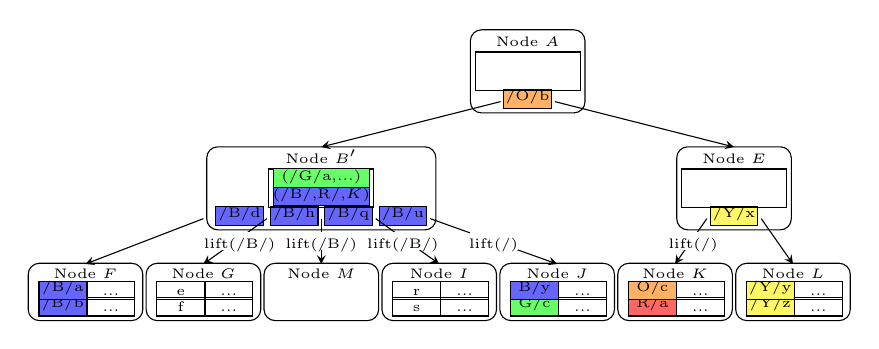
\begin{tikzpicture}[xscale=0.95, yscale=0.95]
            \node[anchor=south, rectangle, rounded corners, minimum height=.06\textwidth, minimum width=.12\textwidth, draw=black] at (0, 0) {};
            \node[anchor=south, font=\tiny] at (0, .036\textwidth) {Node $F$};
            \node[anchor=south, rectangle, minimum height=.015\textwidth, minimum width=.05\textwidth, draw=black, fill={blue!60}] at (-.025\textwidth, .005\textwidth) {};
            \node[anchor=south, font=\tiny] at (-.025\textwidth, 0) {/B/b};
            \node[anchor=south, rectangle, minimum height=.015\textwidth, minimum width=.05\textwidth, draw=black] at (.028\textwidth, .005\textwidth) {};
            \node[anchor=south, font=\tiny] at (.028\textwidth, 0) {...};
            \node[anchor=south, rectangle, minimum height=.015\textwidth, minimum width=.05\textwidth, draw=black, fill={blue!60}] at (-.025\textwidth, .023\textwidth) {};
            \node[anchor=south, font=\tiny] at (-.025\textwidth, .018\textwidth) {/B/a};
            \node[anchor=south, rectangle, minimum height=.015\textwidth, minimum width=.05\textwidth, draw=black] at (.028\textwidth, .023\textwidth) {};
            \node[anchor=south, font=\tiny] at (.028\textwidth, .018\textwidth) {...};

            \node[anchor=south, rectangle, rounded corners, minimum height=.06\textwidth, minimum width=.12\textwidth, draw=black] at (.13\textwidth, 0) {};
            \node[anchor=south, font=\tiny] at (.13\textwidth, .036\textwidth) {Node $G$};
            \node[anchor=south, rectangle, minimum height=.015\textwidth, minimum width=.05\textwidth, draw=black] at (.105\textwidth, .005\textwidth) {};
            \node[anchor=south, font=\tiny] at (.105\textwidth, 0) {f};
            \node[anchor=south, rectangle, minimum height=.015\textwidth, minimum width=.05\textwidth, draw=black] at (.158\textwidth, .005\textwidth) {};
            \node[anchor=south, font=\tiny] at (.158\textwidth, 0) {...};
            \node[anchor=south, rectangle, minimum height=.015\textwidth, minimum width=.05\textwidth, draw=black] at (.105\textwidth, .023\textwidth) {};
            \node[anchor=south, font=\tiny] at (.105\textwidth, .018\textwidth) {e};
            \node[anchor=south, rectangle, minimum height=.015\textwidth, minimum width=.05\textwidth, draw=black] at (.158\textwidth, .023\textwidth) {};
            \node[anchor=south, font=\tiny] at (.158\textwidth, .018\textwidth) {...};

            \node[anchor=south, rectangle, rounded corners, minimum height=.06\textwidth, minimum width=.12\textwidth, draw=black] at (.26\textwidth, 0) {};
            \node[anchor=south, font=\tiny] at (.26\textwidth, .036\textwidth) {Node $M$};

            \node[anchor=south, rectangle, rounded corners, minimum height=.06\textwidth, minimum width=.12\textwidth, draw=black] at (.39\textwidth, 0) {};
            \node[anchor=south, font=\tiny] at (.39\textwidth, .036\textwidth) {Node $I$};
            \node[anchor=south, rectangle, minimum height=.015\textwidth, minimum width=.05\textwidth, draw=black] at (.365\textwidth, .005\textwidth) {};
            \node[anchor=south, font=\tiny] at (.365\textwidth, 0) {s};
            \node[anchor=south, rectangle, minimum height=.015\textwidth, minimum width=.05\textwidth, draw=black] at (.418\textwidth, .005\textwidth) {};
            \node[anchor=south, font=\tiny] at (.418\textwidth, 0) {...};
            \node[anchor=south, rectangle, minimum height=.015\textwidth, minimum width=.05\textwidth, draw=black] at (.365\textwidth, .023\textwidth) {};
            \node[anchor=south, font=\tiny] at (.365\textwidth, .018\textwidth) {r};
            \node[anchor=south, rectangle, minimum height=.015\textwidth, minimum width=.05\textwidth, draw=black] at (.418\textwidth, .023\textwidth) {};
            \node[anchor=south, font=\tiny] at (.418\textwidth, .018\textwidth) {...};

            \node[anchor=south, rectangle, rounded corners, minimum height=.06\textwidth, minimum width=.12\textwidth, draw=black] at (.52\textwidth, 0) {};
            \node[anchor=south, font=\tiny] at (.52\textwidth, .036\textwidth) {Node $J$};
            \node[anchor=south, rectangle, minimum height=.015\textwidth, minimum width=.05\textwidth, draw=black, fill={green!60}] at (.495\textwidth, .005\textwidth) {};
            \node[anchor=south, font=\tiny] at (.495\textwidth, 0) {G/c};
            \node[anchor=south, rectangle, minimum height=.015\textwidth, minimum width=.05\textwidth, draw=black] at (.548\textwidth, .005\textwidth) {};
            \node[anchor=south, font=\tiny] at (.548\textwidth, 0) {...};
            \node[anchor=south, rectangle, minimum height=.015\textwidth, minimum width=.05\textwidth, draw=black, fill={blue!60}] at (.495\textwidth, .023\textwidth) {};
            \node[anchor=south, font=\tiny] at (.495\textwidth, .018\textwidth) {B/y};
            \node[anchor=south, rectangle, minimum height=.015\textwidth, minimum width=.05\textwidth, draw=black] at (.548\textwidth, .023\textwidth) {};
            \node[anchor=south, font=\tiny] at (.548\textwidth, .018\textwidth) {...};

            \node[anchor=south, rectangle, rounded corners, minimum height=.06\textwidth, minimum width=.12\textwidth, draw=black] at (.65\textwidth, 0) {};
            \node[anchor=south, font=\tiny] at (.65\textwidth, .036\textwidth) {Node $K$};
            \node[anchor=south, rectangle, minimum height=.015\textwidth, minimum width=.05\textwidth, draw=black, fill={red!60}] at (.625\textwidth, .005\textwidth) {};
            \node[anchor=south, font=\tiny] at (.625\textwidth, 0) {R/a};
            \node[anchor=south, rectangle, minimum height=.015\textwidth, minimum width=.05\textwidth, draw=black] at (.678\textwidth, .005\textwidth) {};
            \node[anchor=south, font=\tiny] at (.678\textwidth, 0) {...};
            \node[anchor=south, rectangle, minimum height=.015\textwidth, minimum width=.05\textwidth, draw=black, fill={orange!60}] at (.625\textwidth, .023\textwidth) {};
            \node[anchor=south, font=\tiny] at (.625\textwidth, .018\textwidth) {O/c};
            \node[anchor=south, rectangle, minimum height=.015\textwidth, minimum width=.05\textwidth, draw=black] at (.678\textwidth, .023\textwidth) {};
            \node[anchor=south, font=\tiny] at (.678\textwidth, .018\textwidth) {...};

            \node[anchor=south, rectangle, rounded corners, minimum height=.06\textwidth, minimum width=.12\textwidth, draw=black] at (.78\textwidth, 0) {};
            \node[anchor=south, font=\tiny] at (.78\textwidth, .036\textwidth) {Node $L$};
            \node[anchor=south, rectangle, minimum height=.015\textwidth, minimum width=.05\textwidth, draw=black, fill={yellow!60}] at (.755\textwidth, .005\textwidth) {};
            \node[anchor=south, font=\tiny] at (.755\textwidth, 0) {/Y/z};
            \node[anchor=south, rectangle, minimum height=.015\textwidth, minimum width=.05\textwidth, draw=black] at (.808\textwidth, .005\textwidth) {};
            \node[anchor=south, font=\tiny] at (.808\textwidth, 0) {...};
            \node[anchor=south, rectangle, minimum height=.015\textwidth, minimum width=.05\textwidth, draw=black, fill={yellow!60}] at (.755\textwidth, .023\textwidth) {};
            \node[anchor=south, font=\tiny] at (.755\textwidth, .018\textwidth) {/Y/y};
            \node[anchor=south, rectangle, minimum height=.015\textwidth, minimum width=.05\textwidth, draw=black] at (.808\textwidth, .023\textwidth) {};
            \node[anchor=south, font=\tiny] at (.808\textwidth, .018\textwidth) {...};

            \node[anchor=south, rectangle, rounded corners, minimum height=.087\textwidth, minimum width=.24\textwidth, draw=black] at (.26\textwidth, .1\textwidth) {};
            \node[anchor=south, font=\tiny] at (.26\textwidth, .163\textwidth) {Node $B'$};
            \node[anchor=south, rectangle, minimum height=.015\textwidth, minimum width=.05\textwidth, draw=black, fill={blue!60}] at (.17\textwidth, .105\textwidth) {};
            \node[anchor=south, font=\tiny] at (.17\textwidth, .1\textwidth) {/B/d};
            \node[anchor=south, rectangle, minimum height=.015\textwidth, minimum width=.05\textwidth, draw=black, fill={blue!60}] at (.23\textwidth, .105\textwidth) {};
            \node[anchor=south, font=\tiny] at (.23\textwidth, .1\textwidth) {/B/h};
            \node[anchor=south, rectangle, minimum height=.015\textwidth, minimum width=.05\textwidth, draw=black, fill={blue!60}] at (.29\textwidth, .105\textwidth) {};
            \node[anchor=south, font=\tiny] at (.29\textwidth, .1\textwidth) {/B/q};
            \node[anchor=south, rectangle, minimum height=.015\textwidth, minimum width=.05\textwidth, draw=black, fill={blue!60}] at (.35\textwidth, .105\textwidth) {};
            \node[anchor=south, font=\tiny] at (.35\textwidth, .1\textwidth) {/B/u};
            \node[anchor=south, rectangle, minimum height=.04\textwidth, minimum width=.11\textwidth, draw=black] at (.26\textwidth, .125\textwidth) {};
            \node[anchor=south, rectangle, minimum height=.015\textwidth, minimum width=.1\textwidth, draw=black, fill={blue!60}] at (.26\textwidth, .127\textwidth) {};
            \node[anchor=south, font=\tiny] at  (.26\textwidth, .121\textwidth) {\goto(/B/,R/,$K$)};
            \node[anchor=south, rectangle, minimum height=.015\textwidth, minimum width=.1\textwidth, draw=black, fill={green!60}] at (.26\textwidth, .147\textwidth) {};
            \node[anchor=south, font=\tiny] at  (.26\textwidth, .141\textwidth) {\putm(/G/a,...)};

            \node[anchor=south, rectangle, rounded corners, minimum height=.087\textwidth, minimum width=.12\textwidth, draw=black] at (.715\textwidth, .1\textwidth) {};
            \node[anchor=south, font=\tiny] at (.715\textwidth, .163\textwidth) {Node $E$};
            \node[anchor=south, rectangle, minimum height=.015\textwidth, minimum width=.05\textwidth, draw=black, fill={yellow!60}] at (.715\textwidth, .105\textwidth) {};
            \node[anchor=south, font=\tiny] at (.715\textwidth, .1\textwidth) {/Y/x};
            \node[anchor=south, rectangle, minimum height=.04\textwidth, minimum width=.11\textwidth, draw=black] at (.715\textwidth, .125\textwidth) {};

            \node[anchor=south, rectangle, rounded corners, minimum height=.087\textwidth, minimum width=.12\textwidth, draw=black] at (.4875\textwidth, .229\textwidth) {};
            \node[anchor=south, font=\tiny] at (.4875\textwidth, .292\textwidth) {Node $A$};
            \node[anchor=south, rectangle, minimum height=.015\textwidth, minimum width=.05\textwidth, draw=black, fill={orange!60}] at (.4875\textwidth, .234\textwidth) {};
            \node[anchor=south, font=\tiny] at (.4875\textwidth, .229\textwidth) {/O/b};
            \node[anchor=south, rectangle, minimum height=.04\textwidth, minimum width=.11\textwidth, draw=black] at (.4875\textwidth, .254\textwidth) {};

            \draw[->, >=stealth] (.13\textwidth, .113\textwidth) -- (0, .063\textwidth);
            \draw[->, >=stealth] (.20\textwidth, .113\textwidth) -- (.13\textwidth, .063\textwidth);
            \draw[->, >=stealth] (.26\textwidth, .113\textwidth) -- (.26\textwidth, .063\textwidth);
            \draw[->, >=stealth] (.32\textwidth, .113\textwidth) -- (.39\textwidth, .063\textwidth);
            \draw[->, >=stealth] (.38\textwidth, .113\textwidth) -- (.52\textwidth, .063\textwidth);
            \draw[->, >=stealth] (.685\textwidth, .113\textwidth) -- (.65\textwidth, .063\textwidth);
            \draw[->, >=stealth] (.745\textwidth, .113\textwidth) -- (.78\textwidth, .063\textwidth);
            \draw[->, >=stealth] (.4575\textwidth, .242\textwidth) -- (.26\textwidth, .192\textwidth);
            \draw[->, >=stealth] (.5175\textwidth, .242\textwidth) -- (.715\textwidth, .192\textwidth);

            \node[anchor=north,rectangle, minimum height=.015\textwidth, minimum width=.05\textwidth, fill={white}] at (.17\textwidth, .099\textwidth) {};
            \node[anchor=north, font=\tiny] at (.17\textwidth, .102\textwidth) {lift(/B/)};
            \node[anchor=north,rectangle, minimum height=.015\textwidth, minimum width=.05\textwidth, fill={white}] at (.26\textwidth, .099\textwidth) {};
            \node[anchor=north, font=\tiny] at (.26\textwidth, .102\textwidth) {lift(/B/)};
            \node[anchor=north,rectangle, minimum height=.015\textwidth, minimum width=.05\textwidth, fill={white}] at (.35\textwidth, .099\textwidth) {};
            \node[anchor=north, font=\tiny] at (.35\textwidth, .102\textwidth) {lift(/B/)};
            \node[anchor=north,rectangle, minimum height=.015\textwidth, minimum width=.05\textwidth, fill={white}] at (.45\textwidth, .099\textwidth) {};
            \node[anchor=north, font=\tiny] at (.45\textwidth, .102\textwidth) {lift(/)};
            \node[anchor=north,rectangle, minimum height=.015\textwidth, minimum width=.05\textwidth, fill={white}] at (.67\textwidth, .099\textwidth) {};
            \node[anchor=north, font=\tiny] at (.67\textwidth, .102\textwidth) {lift(/)};
        \end{tikzpicture}
        \caption{\label{subfig:flush-3} The lifted \bedag flushes the \goto message
            to Node $B'$.}
    \end{subfigure}
    \caption[The \bedag merges children before flushing a \goto message]{\label{fig:flush}
        When a node tries to flush a \goto message, there may be more than
        one child that overlaps with the key range of the \goto message.
        In this case, the \bedag must merge children to create a single child
        that can accommodate the \goto message.}
\end{figure}

For example, in Figure~\ref{subfig:flush-2}, one child of Node $A$, Node $B'$,
covers the whole key range of the \goto message,
(``/B/$_{min}$'', ``/B/$_{max}$'').
Therefore, the lifted \bedag can flush the \goto message to Node $B'$,
as shown in Figure~\ref{subfig:flush-3}.

In the more complicated case, a \goto message can overlap with the key ranges
of multiple children.
One solution is to duplicate the \goto message and flush to all children.
However,
because duplicating the \goto message increases the reference count of the
source LCA,
the source LCA ends up being shared by many duplicated \goto messages,
making the sharing complicated.

Our solution is to generate a single child that can accommodate the \goto
message.
An easy way is to merge all children whose key range overlaps with the
\goto message.
However, this may create a node with a huge fanout.
In fact, because the \goto message invalidates all old keys
with \dpre, we can decrease the reference counts
(and potentially garbage collect)
of all children whose key ranges fall completely in the key range of the \goto
message (we call these children \textit{interior children})
and merge the two children whose key ranges partly overlap with the
\goto message (we call these two children \textit{fringe children}).

Figure~\ref{fig:flush} shows an example of merging children before flushing a
\goto message.
In Figure~\ref{subfig:flush-1}, Node $B$, $C$ and $D$ all overlap with the
range of the \goto message.
Node $B$ AND $D$ are fringe children, while Node $C$ is an interior child.
Note, though the range-rename operation that generates the \goto message has
``/R/'' as the \spre, the \spre in the \goto message is ``R/'' because ``/'' is
lifted from the source LCA, Node $K$.
To flush the \goto message, in Figure~\ref{subfig:flush-2}, the lifted \bedag
garbage collects Node $C$ and merges Node $B$ and $D$ into Node $B'$.
Note in the example, the merge creates an empty node, Node $M$, to cover the key
range (``/B/h'', ``/B/q'').
After the merge, Node $A$ flushes the \goto message to Node $B'$, as shown in
Figure~\ref{subfig:flush-3}.

In the exmaple, we create an empty node, Node $M$, to cover the key range of
garbage-collected nodes.
Otherwise, we need to enlarge the key range of either Node $G$ or Node $I$.
However, with key lifting, changing the key range of a node means re-lifting
the node and its descendants, which means additioanl I/Os during a flush.

In special cases, there can be only one or no fringe child.
If there is only one fringe child, the flush process removes the interior
children and adds an empty subtree to cover the key range as one child of the
fringe child.
If there is no fringe child, the flush process removes the interior child and
adds an empty subtree to cover the key range as the child of the node.

\paragraph{Converting \goto messages to pivots and parent-to-child pointers.}
After the merging process, there is only one child whose key range overlaps
with the key range of the \goto message.
If the child is higher than the source LCA of the \goto message,
we can simply flush the \goto message to the child buffer.
However, if the child is at the same height as the source LCA,
we cannot flush the \goto message.
In such scenarios, the \goto message is converted into pivots and a
parent-to-child pointer in the node.

The lifted \bedag completes this conversion by adding two new pivots,
\dpre$_{min}$ and \dpre$_{max}$ and
setting the new parent-to-child pointer to the source LCA of the
\goto message.
Assume \dpre$_{min}$ and \dpre$_{max}$ are in the key range of child $i$ of the node,
that is, $\dpre_{min}, \dpre_{max} \in (pivot_{i},pivot_{i+1})$.
Adding \dpre$_{min}$ and \dpre$_{max}$ as two new pivots creates 3 key ranges,
$(pivot_{i},\dpre_{min})$, $(\dpre_{min},\dpre_{max})$ and
$(\dpre_{max}, pivot_{i+1})$.
Key range $(\dpre_{min},\dpre_{max})$ is covered in the source LCA of the \goto
message, while the other two key range are covered by child $i$.

All three parent-to-child pointers now point to children whose key
ranges are different than those specified in the node.
In particular, child $i$ has range $(pivot_{i},pivot_{i+1})$ but bounded by
$(pivot_{i},\dpre_{min})$ or $(\dpre_{max}, pivot_{i+1})$.
The source LCA has a key range that might be larger than
$(\spre_{min}, \spre_{max})$ but bounded by $(\dpre_{min},\dpre_{max})$.
A smaller key range may lift a longer prefix through the parent-to-child
pointer.

The problem is solved by augmenting parent-to-child pointers with \xf functions,
which are the same as the \xf function described in \goto messages.
Each parent-to-child pointer now has a \xf function with a prefix.
After key lifting lifts the search keys of queries by the LCP of two pivots,
the \xf function prepends its prefix to the search key.
Also, \xf functions serves as filters, bounding the results queries may return.

\begin{figure}
    \begin{subfigure}{\textwidth}
        \centering
        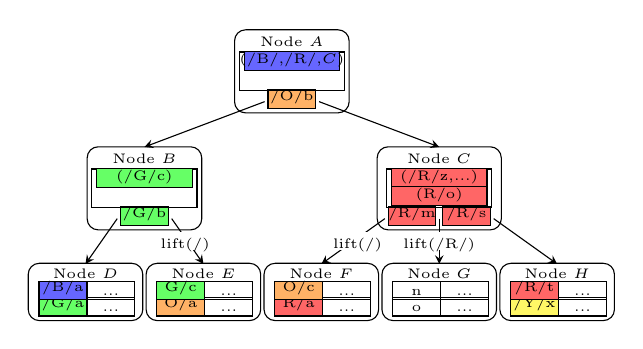
\begin{tikzpicture}[xscale=0.95, yscale=0.95]
            \node[anchor=south, rectangle, rounded corners, minimum height=.06\textwidth, minimum width=.12\textwidth, draw=black] at (0, 0) {};
            \node[anchor=south, font=\tiny] at (0, .036\textwidth) {Node $F$};
            \node[anchor=south, rectangle, minimum height=.015\textwidth, minimum width=.05\textwidth, draw=black, fill={red!60}] at (-.025\textwidth, .005\textwidth) {};
            \node[anchor=south, font=\tiny] at (-.025\textwidth, 0) {R/a};
            \node[anchor=south, rectangle, minimum height=.015\textwidth, minimum width=.05\textwidth, draw=black] at (.028\textwidth, .005\textwidth) {};
            \node[anchor=south, font=\tiny] at (.028\textwidth, 0) {...};
            \node[anchor=south, rectangle, minimum height=.015\textwidth, minimum width=.05\textwidth, draw=black, fill={orange!60}] at (-.025\textwidth, .023\textwidth) {};
            \node[anchor=south, font=\tiny] at (-.025\textwidth, .018\textwidth) {O/c};
            \node[anchor=south, rectangle, minimum height=.015\textwidth, minimum width=.05\textwidth, draw=black] at (.028\textwidth, .023\textwidth) {};
            \node[anchor=south, font=\tiny] at (.028\textwidth, .018\textwidth) {...};

            \node[anchor=south, rectangle, rounded corners, minimum height=.06\textwidth, minimum width=.12\textwidth, draw=black] at (.13\textwidth, 0) {};
            \node[anchor=south, font=\tiny] at (.13\textwidth, .036\textwidth) {Node $G$};
            \node[anchor=south, rectangle, minimum height=.015\textwidth, minimum width=.05\textwidth, draw=black] at (.105\textwidth, .005\textwidth) {};
            \node[anchor=south, font=\tiny] at (.105\textwidth, 0) {o};
            \node[anchor=south, rectangle, minimum height=.015\textwidth, minimum width=.05\textwidth, draw=black] at (.158\textwidth, .005\textwidth) {};
            \node[anchor=south, font=\tiny] at (.158\textwidth, 0) {...};
            \node[anchor=south, rectangle, minimum height=.015\textwidth, minimum width=.05\textwidth, draw=black] at (.105\textwidth, .023\textwidth) {};
            \node[anchor=south, font=\tiny] at (.105\textwidth, .018\textwidth) {n};
            \node[anchor=south, rectangle, minimum height=.015\textwidth, minimum width=.05\textwidth, draw=black] at (.158\textwidth, .023\textwidth) {};
            \node[anchor=south, font=\tiny] at (.158\textwidth, .018\textwidth) {...};

            \node[anchor=south, rectangle, rounded corners, minimum height=.06\textwidth, minimum width=.12\textwidth, draw=black] at (.26\textwidth, 0) {};
            \node[anchor=south, font=\tiny] at (.26\textwidth, .036\textwidth) {Node $H$};
            \node[anchor=south, rectangle, minimum height=.015\textwidth, minimum width=.05\textwidth, draw=black, fill={yellow!60}] at (.235\textwidth, .005\textwidth) {};
            \node[anchor=south, font=\tiny] at (.235\textwidth, 0) {/Y/x};
            \node[anchor=south, rectangle, minimum height=.015\textwidth, minimum width=.05\textwidth, draw=black] at (.288\textwidth, .005\textwidth) {};
            \node[anchor=south, font=\tiny] at (.288\textwidth, 0) {...};
            \node[anchor=south, rectangle, minimum height=.015\textwidth, minimum width=.05\textwidth, draw=black, fill={red!60}] at (.235\textwidth, .023\textwidth) {};
            \node[anchor=south, font=\tiny] at (.235\textwidth, .018\textwidth) {/R/t};
            \node[anchor=south, rectangle, minimum height=.015\textwidth, minimum width=.05\textwidth, draw=black] at (.288\textwidth, .023\textwidth) {};
            \node[anchor=south, font=\tiny] at (.288\textwidth, .018\textwidth) {...};

            \node[anchor=south, rectangle, rounded corners, minimum height=.06\textwidth, minimum width=.12\textwidth, draw=black] at (-.13\textwidth, 0) {};
            \node[anchor=south, font=\tiny] at (-.13\textwidth, .036\textwidth) {Node $E$};
            \node[anchor=south, rectangle, minimum height=.015\textwidth, minimum width=.05\textwidth, draw=black, fill={orange!60}] at (-.155\textwidth, .005\textwidth) {};
            \node[anchor=south, font=\tiny] at (-.155\textwidth, 0) {O/a};
            \node[anchor=south, rectangle, minimum height=.015\textwidth, minimum width=.05\textwidth, draw=black] at (-.102\textwidth, .005\textwidth) {};
            \node[anchor=south, font=\tiny] at (-.102\textwidth, 0) {...};
            \node[anchor=south, rectangle, minimum height=.015\textwidth, minimum width=.05\textwidth, draw=black, fill={green!60}] at (-.155\textwidth, .023\textwidth) {};
            \node[anchor=south, font=\tiny] at (-.155\textwidth, .018\textwidth) {G/c};
            \node[anchor=south, rectangle, minimum height=.015\textwidth, minimum width=.05\textwidth, draw=black] at (-.102\textwidth, .023\textwidth) {};
            \node[anchor=south, font=\tiny] at (-.102\textwidth, .018\textwidth) {...};

            \node[anchor=south, rectangle, rounded corners, minimum height=.06\textwidth, minimum width=.12\textwidth, draw=black] at (-.26\textwidth, 0) {};
            \node[anchor=south, font=\tiny] at (-.26\textwidth, .036\textwidth) {Node $D$};
            \node[anchor=south, rectangle, minimum height=.015\textwidth, minimum width=.05\textwidth, draw=black, fill={green!60}] at (-.285\textwidth, .005\textwidth) {};
            \node[anchor=south, font=\tiny] at (-.285\textwidth, 0) {/G/a};
            \node[anchor=south, rectangle, minimum height=.015\textwidth, minimum width=.05\textwidth, draw=black] at (-.232\textwidth, .005\textwidth) {};
            \node[anchor=south, font=\tiny] at (-.232\textwidth, 0) {...};
            \node[anchor=south, rectangle, minimum height=.015\textwidth, minimum width=.05\textwidth, draw=black, fill={blue!60}] at (-.285\textwidth, .023\textwidth) {};
            \node[anchor=south, font=\tiny] at (-.285\textwidth, .018\textwidth) {/B/a};
            \node[anchor=south, rectangle, minimum height=.015\textwidth, minimum width=.05\textwidth, draw=black] at (-.232\textwidth, .023\textwidth) {};
            \node[anchor=south, font=\tiny] at (-.232\textwidth, .018\textwidth) {...};

            \node[anchor=south, rectangle, rounded corners, minimum height=.087\textwidth, minimum width=.12\textwidth, draw=black] at (-.195\textwidth, .1\textwidth) {};
            \node[anchor=south, font=\tiny] at (-.195\textwidth, .163\textwidth) {Node $B$};
            \node[anchor=south, rectangle, minimum height=.015\textwidth, minimum width=.05\textwidth, draw=black, fill={green!60}] at (-.195\textwidth, .105\textwidth) {};
            \node[anchor=south, font=\tiny] at (-.195\textwidth, .1\textwidth) {/G/b};
            \node[anchor=south, rectangle, minimum height=.04\textwidth, minimum width=.11\textwidth, draw=black] at (-.195\textwidth, .125\textwidth) {};
            \node[anchor=south, rectangle, minimum height=.015\textwidth, minimum width=.1\textwidth, draw=black, fill={green!60}] at (-.195\textwidth, .147\textwidth) {};
            \node[anchor=south, font=\tiny] at  (-.195\textwidth, .141\textwidth) {\delm(/G/c)};

            \node[anchor=south, rectangle, rounded corners, minimum height=.087\textwidth, minimum width=.13\textwidth, draw=black] at (.13\textwidth, .1\textwidth) {};
            \node[anchor=south, font=\tiny] at (.13\textwidth, .163\textwidth) {Node $C$};
            \node[anchor=south, rectangle, minimum height=.015\textwidth, minimum width=.05\textwidth, draw=black, fill={red!60}] at (.1\textwidth, .105\textwidth) {};
            \node[anchor=south, font=\tiny] at (.1\textwidth, .1\textwidth) {/R/m};
            \node[anchor=south, rectangle, minimum height=.015\textwidth, minimum width=.05\textwidth, draw=black, fill={red!60}] at (.16\textwidth, .105\textwidth) {};
            \node[anchor=south, font=\tiny] at (.16\textwidth, .1\textwidth) {/R/s};
            \node[anchor=south, rectangle, minimum height=.04\textwidth, minimum width=.11\textwidth, draw=black] at (.13\textwidth, .125\textwidth) {};
            \node[anchor=south, rectangle, minimum height=.015\textwidth, minimum width=.1\textwidth, draw=black, fill={red!60}] at (.13\textwidth, .147\textwidth) {};
            \node[anchor=south, font=\tiny] at  (.13\textwidth, .141\textwidth) {\putm(/R/z,...)};
            \node[anchor=south, rectangle, minimum height=.015\textwidth, minimum width=.1\textwidth, draw=black, fill={red!60}] at (.13\textwidth, .127\textwidth) {};
            \node[anchor=south, font=\tiny] at  (.13\textwidth, .121\textwidth) {\delm(R/o)};

            \node[anchor=south, rectangle, rounded corners, minimum height=.087\textwidth, minimum width=.12\textwidth, draw=black] at (-.0325\textwidth, .229\textwidth) {};
            \node[anchor=south, font=\tiny] at (-.0325\textwidth, .292\textwidth) {Node $A$};
            \node[anchor=south, rectangle, minimum height=.015\textwidth, minimum width=.05\textwidth, draw=black, fill={orange!60}] at (-.0325\textwidth, .234\textwidth) {};
            \node[anchor=south, font=\tiny] at (-.0325\textwidth, .229\textwidth) {/O/b};
            \node[anchor=south, rectangle, minimum height=.04\textwidth, minimum width=.11\textwidth, draw=black] at (-.0325\textwidth, .254\textwidth) {};
            \node[anchor=south, rectangle, minimum height=.015\textwidth, minimum width=.1\textwidth, draw=black, fill={blue!60}] at (-.0325\textwidth, .276\textwidth) {};
            \node[anchor=south, font=\tiny] at  (-.0325\textwidth, .27\textwidth) {\goto(/B/,/R/,$C$)};

            \draw[->, >=stealth] (-.225\textwidth, .113\textwidth) -- (-.26\textwidth, .063\textwidth);
            \draw[->, >=stealth] (-.165\textwidth, .113\textwidth) -- (-.13\textwidth, .063\textwidth);
            \draw[->, >=stealth] (.13\textwidth, .113\textwidth) -- (.13\textwidth, .063\textwidth);
            \draw[->, >=stealth] (.19\textwidth, .113\textwidth) -- (.26\textwidth, .063\textwidth);
            \draw[->, >=stealth] (.07\textwidth, .113\textwidth) -- (0, .063\textwidth);
            \draw[->, >=stealth] (-.0625\textwidth, .242\textwidth) -- (-.195\textwidth, .192\textwidth);
            \draw[->, >=stealth] (-.0025\textwidth, .242\textwidth) -- (.13\textwidth, .192\textwidth);

            \node[anchor=north,rectangle, minimum height=.015\textwidth, minimum width=.05\textwidth, fill={white}] at (.13\textwidth, .099\textwidth) {};
            \node[anchor=north, font=\tiny] at (.13\textwidth, .102\textwidth) {lift(/R/)};
            \node[anchor=north,rectangle, minimum height=.015\textwidth, minimum width=.05\textwidth, fill={white}] at (.04\textwidth, .099\textwidth) {};
            \node[anchor=north, font=\tiny] at (.04\textwidth, .102\textwidth) {lift(/)};
            \node[anchor=north,rectangle, minimum height=.015\textwidth, minimum width=.05\textwidth, fill={white}] at (-.15\textwidth, .099\textwidth) {};
            \node[anchor=north, font=\tiny] at (-.15\textwidth, .102\textwidth) {lift(/)};
        \end{tikzpicture}
        \caption{\label{subfig:spvt-1} The \goto message cannot be flushed to
            Node $B$, which is at the same as Node $C$.}
    \end{subfigure}
    \begin{subfigure}{\textwidth}
        \centering
        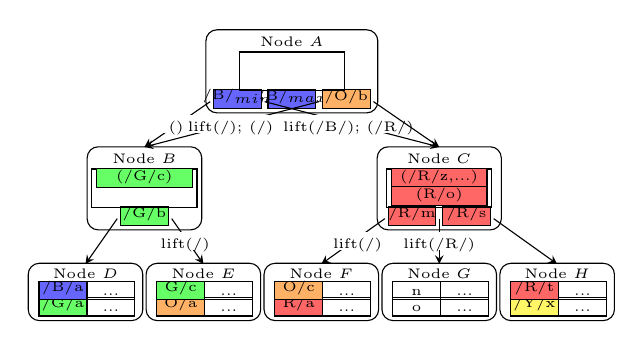
\begin{tikzpicture}[xscale=0.95, yscale=0.95]
            \node[anchor=south, rectangle, rounded corners, minimum height=.06\textwidth, minimum width=.12\textwidth, draw=black] at (0, 0) {};
            \node[anchor=south, font=\tiny] at (0, .036\textwidth) {Node $F$};
            \node[anchor=south, rectangle, minimum height=.015\textwidth, minimum width=.05\textwidth, draw=black, fill={red!60}] at (-.025\textwidth, .005\textwidth) {};
            \node[anchor=south, font=\tiny] at (-.025\textwidth, 0) {R/a};
            \node[anchor=south, rectangle, minimum height=.015\textwidth, minimum width=.05\textwidth, draw=black] at (.028\textwidth, .005\textwidth) {};
            \node[anchor=south, font=\tiny] at (.028\textwidth, 0) {...};
            \node[anchor=south, rectangle, minimum height=.015\textwidth, minimum width=.05\textwidth, draw=black, fill={orange!60}] at (-.025\textwidth, .023\textwidth) {};
            \node[anchor=south, font=\tiny] at (-.025\textwidth, .018\textwidth) {O/c};
            \node[anchor=south, rectangle, minimum height=.015\textwidth, minimum width=.05\textwidth, draw=black] at (.028\textwidth, .023\textwidth) {};
            \node[anchor=south, font=\tiny] at (.028\textwidth, .018\textwidth) {...};

            \node[anchor=south, rectangle, rounded corners, minimum height=.06\textwidth, minimum width=.12\textwidth, draw=black] at (.13\textwidth, 0) {};
            \node[anchor=south, font=\tiny] at (.13\textwidth, .036\textwidth) {Node $G$};
            \node[anchor=south, rectangle, minimum height=.015\textwidth, minimum width=.05\textwidth, draw=black] at (.105\textwidth, .005\textwidth) {};
            \node[anchor=south, font=\tiny] at (.105\textwidth, 0) {o};
            \node[anchor=south, rectangle, minimum height=.015\textwidth, minimum width=.05\textwidth, draw=black] at (.158\textwidth, .005\textwidth) {};
            \node[anchor=south, font=\tiny] at (.158\textwidth, 0) {...};
            \node[anchor=south, rectangle, minimum height=.015\textwidth, minimum width=.05\textwidth, draw=black] at (.105\textwidth, .023\textwidth) {};
            \node[anchor=south, font=\tiny] at (.105\textwidth, .018\textwidth) {n};
            \node[anchor=south, rectangle, minimum height=.015\textwidth, minimum width=.05\textwidth, draw=black] at (.158\textwidth, .023\textwidth) {};
            \node[anchor=south, font=\tiny] at (.158\textwidth, .018\textwidth) {...};

            \node[anchor=south, rectangle, rounded corners, minimum height=.06\textwidth, minimum width=.12\textwidth, draw=black] at (.26\textwidth, 0) {};
            \node[anchor=south, font=\tiny] at (.26\textwidth, .036\textwidth) {Node $H$};
            \node[anchor=south, rectangle, minimum height=.015\textwidth, minimum width=.05\textwidth, draw=black, fill={yellow!60}] at (.235\textwidth, .005\textwidth) {};
            \node[anchor=south, font=\tiny] at (.235\textwidth, 0) {/Y/x};
            \node[anchor=south, rectangle, minimum height=.015\textwidth, minimum width=.05\textwidth, draw=black] at (.288\textwidth, .005\textwidth) {};
            \node[anchor=south, font=\tiny] at (.288\textwidth, 0) {...};
            \node[anchor=south, rectangle, minimum height=.015\textwidth, minimum width=.05\textwidth, draw=black, fill={red!60}] at (.235\textwidth, .023\textwidth) {};
            \node[anchor=south, font=\tiny] at (.235\textwidth, .018\textwidth) {/R/t};
            \node[anchor=south, rectangle, minimum height=.015\textwidth, minimum width=.05\textwidth, draw=black] at (.288\textwidth, .023\textwidth) {};
            \node[anchor=south, font=\tiny] at (.288\textwidth, .018\textwidth) {...};

            \node[anchor=south, rectangle, rounded corners, minimum height=.06\textwidth, minimum width=.12\textwidth, draw=black] at (-.13\textwidth, 0) {};
            \node[anchor=south, font=\tiny] at (-.13\textwidth, .036\textwidth) {Node $E$};
            \node[anchor=south, rectangle, minimum height=.015\textwidth, minimum width=.05\textwidth, draw=black, fill={orange!60}] at (-.155\textwidth, .005\textwidth) {};
            \node[anchor=south, font=\tiny] at (-.155\textwidth, 0) {O/a};
            \node[anchor=south, rectangle, minimum height=.015\textwidth, minimum width=.05\textwidth, draw=black] at (-.102\textwidth, .005\textwidth) {};
            \node[anchor=south, font=\tiny] at (-.102\textwidth, 0) {...};
            \node[anchor=south, rectangle, minimum height=.015\textwidth, minimum width=.05\textwidth, draw=black, fill={green!60}] at (-.155\textwidth, .023\textwidth) {};
            \node[anchor=south, font=\tiny] at (-.155\textwidth, .018\textwidth) {G/c};
            \node[anchor=south, rectangle, minimum height=.015\textwidth, minimum width=.05\textwidth, draw=black] at (-.102\textwidth, .023\textwidth) {};
            \node[anchor=south, font=\tiny] at (-.102\textwidth, .018\textwidth) {...};

            \node[anchor=south, rectangle, rounded corners, minimum height=.06\textwidth, minimum width=.12\textwidth, draw=black] at (-.26\textwidth, 0) {};
            \node[anchor=south, font=\tiny] at (-.26\textwidth, .036\textwidth) {Node $D$};
            \node[anchor=south, rectangle, minimum height=.015\textwidth, minimum width=.05\textwidth, draw=black, fill={green!60}] at (-.285\textwidth, .005\textwidth) {};
            \node[anchor=south, font=\tiny] at (-.285\textwidth, 0) {/G/a};
            \node[anchor=south, rectangle, minimum height=.015\textwidth, minimum width=.05\textwidth, draw=black] at (-.232\textwidth, .005\textwidth) {};
            \node[anchor=south, font=\tiny] at (-.232\textwidth, 0) {...};
            \node[anchor=south, rectangle, minimum height=.015\textwidth, minimum width=.05\textwidth, draw=black, fill={blue!60}] at (-.285\textwidth, .023\textwidth) {};
            \node[anchor=south, font=\tiny] at (-.285\textwidth, .018\textwidth) {/B/a};
            \node[anchor=south, rectangle, minimum height=.015\textwidth, minimum width=.05\textwidth, draw=black] at (-.232\textwidth, .023\textwidth) {};
            \node[anchor=south, font=\tiny] at (-.232\textwidth, .018\textwidth) {...};

            \node[anchor=south, rectangle, rounded corners, minimum height=.087\textwidth, minimum width=.12\textwidth, draw=black] at (-.195\textwidth, .1\textwidth) {};
            \node[anchor=south, font=\tiny] at (-.195\textwidth, .163\textwidth) {Node $B$};
            \node[anchor=south, rectangle, minimum height=.015\textwidth, minimum width=.05\textwidth, draw=black, fill={green!60}] at (-.195\textwidth, .105\textwidth) {};
            \node[anchor=south, font=\tiny] at (-.195\textwidth, .1\textwidth) {/G/b};
            \node[anchor=south, rectangle, minimum height=.04\textwidth, minimum width=.11\textwidth, draw=black] at (-.195\textwidth, .125\textwidth) {};
            \node[anchor=south, rectangle, minimum height=.015\textwidth, minimum width=.1\textwidth, draw=black, fill={green!60}] at (-.195\textwidth, .147\textwidth) {};
            \node[anchor=south, font=\tiny] at  (-.195\textwidth, .141\textwidth) {\delm(/G/c)};

            \node[anchor=south, rectangle, rounded corners, minimum height=.087\textwidth, minimum width=.13\textwidth, draw=black] at (.13\textwidth, .1\textwidth) {};
            \node[anchor=south, font=\tiny] at (.13\textwidth, .163\textwidth) {Node $C$};
            \node[anchor=south, rectangle, minimum height=.015\textwidth, minimum width=.05\textwidth, draw=black, fill={red!60}] at (.1\textwidth, .105\textwidth) {};
            \node[anchor=south, font=\tiny] at (.1\textwidth, .1\textwidth) {/R/m};
            \node[anchor=south, rectangle, minimum height=.015\textwidth, minimum width=.05\textwidth, draw=black, fill={red!60}] at (.16\textwidth, .105\textwidth) {};
            \node[anchor=south, font=\tiny] at (.16\textwidth, .1\textwidth) {/R/s};
            \node[anchor=south, rectangle, minimum height=.04\textwidth, minimum width=.11\textwidth, draw=black] at (.13\textwidth, .125\textwidth) {};
            \node[anchor=south, rectangle, minimum height=.015\textwidth, minimum width=.1\textwidth, draw=black, fill={red!60}] at (.13\textwidth, .147\textwidth) {};
            \node[anchor=south, font=\tiny] at  (.13\textwidth, .141\textwidth) {\putm(/R/z,...)};
            \node[anchor=south, rectangle, minimum height=.015\textwidth, minimum width=.1\textwidth, draw=black, fill={red!60}] at (.13\textwidth, .127\textwidth) {};
            \node[anchor=south, font=\tiny] at  (.13\textwidth, .121\textwidth) {\delm(R/o)};

            \node[anchor=south, rectangle, rounded corners, minimum height=.087\textwidth, minimum width=.18\textwidth, draw=black] at (-.0325\textwidth, .229\textwidth) {};
            \node[anchor=south, font=\tiny] at (-.0325\textwidth, .292\textwidth) {Node $A$};
            \node[anchor=south, rectangle, minimum height=.015\textwidth, minimum width=.05\textwidth, draw=black, fill={blue!60}] at (-.0325\textwidth, .234\textwidth) {};
            \node[anchor=south, font=\tiny] at (-.0325\textwidth, .229\textwidth) {/B/$_{max}$};
            \node[anchor=south, rectangle, minimum height=.015\textwidth, minimum width=.05\textwidth, draw=black, fill={blue!60}] at (-.0925\textwidth, .234\textwidth) {};
            \node[anchor=south, font=\tiny] at (-.0925\textwidth, .229\textwidth) {/B/$_{min}$};
            \node[anchor=south, rectangle, minimum height=.015\textwidth, minimum width=.05\textwidth, draw=black, fill={orange!60}] at (.0275\textwidth, .234\textwidth) {};
            \node[anchor=south, font=\tiny] at (.0275\textwidth, .229\textwidth) {/O/b};
            \node[anchor=south, rectangle, minimum height=.04\textwidth, minimum width=.11\textwidth, draw=black] at (-.0325\textwidth, .254\textwidth) {};

            \draw[->, >=stealth] (-.225\textwidth, .113\textwidth) -- (-.26\textwidth, .063\textwidth);
            \draw[->, >=stealth] (-.165\textwidth, .113\textwidth) -- (-.13\textwidth, .063\textwidth);
            \draw[->, >=stealth] (.13\textwidth, .113\textwidth) -- (.13\textwidth, .063\textwidth);
            \draw[->, >=stealth] (.19\textwidth, .113\textwidth) -- (.26\textwidth, .063\textwidth);
            \draw[->, >=stealth] (.07\textwidth, .113\textwidth) -- (0, .063\textwidth);
            \draw[->, >=stealth] (-.1225\textwidth, .242\textwidth) -- (-.195\textwidth, .192\textwidth);
            \draw[->, >=stealth] (-.0625\textwidth, .242\textwidth) -- (.13\textwidth, .192\textwidth);
            \draw[->, >=stealth] (-.0025\textwidth, .242\textwidth) -- (-.195\textwidth, .192\textwidth);
            \draw[->, >=stealth] (.0575\textwidth, .242\textwidth) -- (.13\textwidth, .192\textwidth);

            \node[anchor=north,rectangle, minimum height=.015\textwidth, minimum width=.05\textwidth, fill={white}] at (.13\textwidth, .099\textwidth) {};
            \node[anchor=north, font=\tiny] at (.13\textwidth, .102\textwidth) {lift(/R/)};
            \node[anchor=north,rectangle, minimum height=.015\textwidth, minimum width=.05\textwidth, fill={white}] at (.04\textwidth, .099\textwidth) {};
            \node[anchor=north, font=\tiny] at (.04\textwidth, .102\textwidth) {lift(/)};
            \node[anchor=north,rectangle, minimum height=.015\textwidth, minimum width=.05\textwidth, fill={white}] at (-.15\textwidth, .099\textwidth) {};
            \node[anchor=north, font=\tiny] at (-.15\textwidth, .102\textwidth) {lift(/)};
            \node[anchor=north,rectangle, minimum height=.015\textwidth, minimum width=.05\textwidth, fill={white}] at (-.16\textwidth, .228\textwidth) {};
            \node[anchor=north, font=\tiny] at (-.16\textwidth, .231\textwidth) {\xf ()};
            \node[anchor=north,rectangle, minimum height=.015\textwidth, minimum width=.08\textwidth, fill={white}] at (-.1\textwidth, .228\textwidth) {};
            \node[anchor=north, font=\tiny] at (-.1\textwidth, .231\textwidth) {lift(/); \xf (/)};
            \node[anchor=north,rectangle, minimum height=.015\textwidth, minimum width=.08\textwidth, fill={white}] at (.03\textwidth, .228\textwidth) {};
            \node[anchor=north, font=\tiny] at (.03\textwidth, .231\textwidth) {lift(/B/); \xf (/R/)};
        \end{tikzpicture}
        \caption{\label{subfig:spvt-2} The \goto message becomes pivots and a
            parent-to-child pointer, and adds \xf functions to the parent-to-child pointers.}
    \end{subfigure}
    \caption[Transform a \goto message into pivots and a parent-to-child pointer]{\label{fig:spvt}
        When the lifted \bedag cannot flush a \goto message deeper, it
        transforms the \goto message into pivots and a parent-to-child pointers
        and adds \xf functions to the parent-to-child pointers.}
\end{figure}

Figure~\ref{fig:spvt} shows an example of the transformation.
The lifted \bedag cannot flush the \goto message from Node $A$ to Node $B$,
because Node $B$ is at the same height as its source LCA, Node $C$.
Therefore, two pivots, ``/B/$_{min}$'' and ``/B/$_{max}$'', are added to Node $A$.
The parent-to-child pointer between ``/B/$_{min}$'' and ``/B/$_{max}$'' points
to the source LCA, Node $C$, and has a \xf function of ``/R/'', indicating a
key range mismatch and the additional prefix ``/R/'' for keys in the child.
Queries following that parent-to-child pointer should prepend prefix ``/R/''
after the normal lifting of ``/B/'' from its search key.
Also, queries remember only keys between ``/R/$_{min}$'' and ``/R/$_{max}$'' in
the child are valid.
Similarly, two \xf functions are added to the other two pointers.
Note, for the leftmost parent-to-child pointer of Node $A$, though the \xf
function contains no prefix, it still serves as a filter for queries.

With the help of \xf functions in parent-to-child pointers,
the \bedag can transfer a \goto message into two pivots and a parent-to-child
pointer.
Now, let's look at how \xf functions are resolved during flushes,
finishing the rest work in the range-clone operation.

\paragraph{Fixing \xf functions in parent-to-child pointers.}
\goto messages add \xf functions to parent-to-child pointers.
The \xf function transforms the search keys of queries by prepending its prefix
after normal key lifting through parent-to-child pointers.
Also, the \xf function indicates that
the child contains keys outside of the key range
specified by pivots in the parent and
thus, queries should ignore those keys following
the parent-to-child pointers.

The lifted \bedag resolves \xf functions through node flushes.
Specifically, when flushing from a parent to a child and the parent-to-child
pointer has an \xf function,
the lifted \bedag garbage collects exterior children of the child whose key
ranges are completely outside of the key range specified by the pivots in parent.
Also, the lifted \bedag removes messages whose keys are outside of the key
range specified in the parent from the child buffer.
Then, for fringe children whose key ranges partly overlap with that specified
in the parent, the \bedag propagates the \xf function to their parent-to-child
pointers.
Finally, if the \xf function has a prefix, the \bedag lifts the prefix from
keys in the child.

\begin{figure}
    \begin{subfigure}{\textwidth}
        \centering
        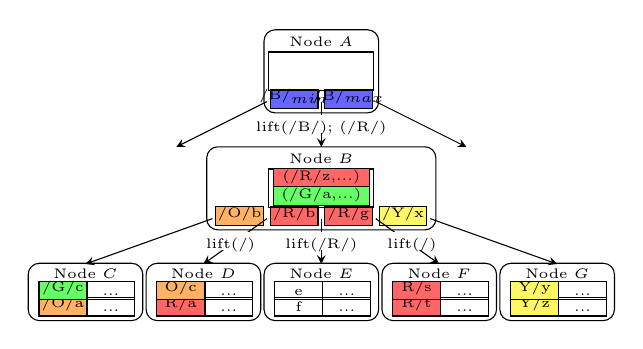
\begin{tikzpicture}[xscale=0.95, yscale=0.95]
            \node[anchor=south, rectangle, rounded corners, minimum height=.06\textwidth, minimum width=.12\textwidth, draw=black] at (0, 0) {};
            \node[anchor=south, font=\tiny] at (0, .036\textwidth) {Node $C$};
            \node[anchor=south, rectangle, minimum height=.015\textwidth, minimum width=.05\textwidth, draw=black, fill={orange!60}] at (-.025\textwidth, .005\textwidth) {};
            \node[anchor=south, font=\tiny] at (-.025\textwidth, 0) {/O/a};
            \node[anchor=south, rectangle, minimum height=.015\textwidth, minimum width=.05\textwidth, draw=black] at (.028\textwidth, .005\textwidth) {};
            \node[anchor=south, font=\tiny] at (.028\textwidth, 0) {...};
            \node[anchor=south, rectangle, minimum height=.015\textwidth, minimum width=.05\textwidth, draw=black, fill={green!60}] at (-.025\textwidth, .023\textwidth) {};
            \node[anchor=south, font=\tiny] at (-.025\textwidth, .018\textwidth) {/G/c};
            \node[anchor=south, rectangle, minimum height=.015\textwidth, minimum width=.05\textwidth, draw=black] at (.028\textwidth, .023\textwidth) {};
            \node[anchor=south, font=\tiny] at (.028\textwidth, .018\textwidth) {...};

            \node[anchor=south, rectangle, rounded corners, minimum height=.06\textwidth, minimum width=.12\textwidth, draw=black] at (.13\textwidth, 0) {};
            \node[anchor=south, font=\tiny] at (.13\textwidth, .036\textwidth) {Node $D$};
            \node[anchor=south, rectangle, minimum height=.015\textwidth, minimum width=.05\textwidth, draw=black, fill={red!60}] at (.105\textwidth, .005\textwidth) {};
            \node[anchor=south, font=\tiny] at (.105\textwidth, 0) {R/a};
            \node[anchor=south, rectangle, minimum height=.015\textwidth, minimum width=.05\textwidth, draw=black] at (.158\textwidth, .005\textwidth) {};
            \node[anchor=south, font=\tiny] at (.158\textwidth, 0) {...};
            \node[anchor=south, rectangle, minimum height=.015\textwidth, minimum width=.05\textwidth, draw=black, fill={orange!60}] at (.105\textwidth, .023\textwidth) {};
            \node[anchor=south, font=\tiny] at (.105\textwidth, .018\textwidth) {O/c};
            \node[anchor=south, rectangle, minimum height=.015\textwidth, minimum width=.05\textwidth, draw=black] at (.158\textwidth, .023\textwidth) {};
            \node[anchor=south, font=\tiny] at (.158\textwidth, .018\textwidth) {...};

            \node[anchor=south, rectangle, rounded corners, minimum height=.06\textwidth, minimum width=.12\textwidth, draw=black] at (.26\textwidth, 0) {};
            \node[anchor=south, font=\tiny] at (.26\textwidth, .036\textwidth) {Node $E$};
            \node[anchor=south, rectangle, minimum height=.015\textwidth, minimum width=.05\textwidth, draw=black] at (.235\textwidth, .005\textwidth) {};
            \node[anchor=south, font=\tiny] at (.235\textwidth, 0) {f};
            \node[anchor=south, rectangle, minimum height=.015\textwidth, minimum width=.05\textwidth, draw=black] at (.288\textwidth, .005\textwidth) {};
            \node[anchor=south, font=\tiny] at (.288\textwidth, 0) {...};
            \node[anchor=south, rectangle, minimum height=.015\textwidth, minimum width=.05\textwidth, draw=black] at (.235\textwidth, .023\textwidth) {};
            \node[anchor=south, font=\tiny] at (.235\textwidth, .018\textwidth) {e};
            \node[anchor=south, rectangle, minimum height=.015\textwidth, minimum width=.05\textwidth, draw=black] at (.288\textwidth, .023\textwidth) {};
            \node[anchor=south, font=\tiny] at (.288\textwidth, .018\textwidth) {...};

            \node[anchor=south, rectangle, rounded corners, minimum height=.06\textwidth, minimum width=.12\textwidth, draw=black] at (.39\textwidth, 0) {};
            \node[anchor=south, font=\tiny] at (.39\textwidth, .036\textwidth) {Node $F$};
            \node[anchor=south, rectangle, minimum height=.015\textwidth, minimum width=.05\textwidth, draw=black, fill={red!60}] at (.365\textwidth, .005\textwidth) {};
            \node[anchor=south, font=\tiny] at (.365\textwidth, 0) {R/t};
            \node[anchor=south, rectangle, minimum height=.015\textwidth, minimum width=.05\textwidth, draw=black] at (.418\textwidth, .005\textwidth) {};
            \node[anchor=south, font=\tiny] at (.418\textwidth, 0) {...};
            \node[anchor=south, rectangle, minimum height=.015\textwidth, minimum width=.05\textwidth, draw=black, fill={red!60}] at (.365\textwidth, .023\textwidth) {};
            \node[anchor=south, font=\tiny] at (.365\textwidth, .018\textwidth) {R/s};
            \node[anchor=south, rectangle, minimum height=.015\textwidth, minimum width=.05\textwidth, draw=black] at (.418\textwidth, .023\textwidth) {};
            \node[anchor=south, font=\tiny] at (.418\textwidth, .018\textwidth) {...};

            \node[anchor=south, rectangle, rounded corners, minimum height=.06\textwidth, minimum width=.12\textwidth, draw=black] at (.52\textwidth, 0) {};
            \node[anchor=south, font=\tiny] at (.52\textwidth, .036\textwidth) {Node $G$};
            \node[anchor=south, rectangle, minimum height=.015\textwidth, minimum width=.05\textwidth, draw=black, fill={yellow!60}] at (.495\textwidth, .005\textwidth) {};
            \node[anchor=south, font=\tiny] at (.495\textwidth, 0) {Y/z};
            \node[anchor=south, rectangle, minimum height=.015\textwidth, minimum width=.05\textwidth, draw=black] at (.548\textwidth, .005\textwidth) {};
            \node[anchor=south, font=\tiny] at (.548\textwidth, 0) {...};
            \node[anchor=south, rectangle, minimum height=.015\textwidth, minimum width=.05\textwidth, draw=black, fill={yellow!60}] at (.495\textwidth, .023\textwidth) {};
            \node[anchor=south, font=\tiny] at (.495\textwidth, .018\textwidth) {Y/y};
            \node[anchor=south, rectangle, minimum height=.015\textwidth, minimum width=.05\textwidth, draw=black] at (.548\textwidth, .023\textwidth) {};
            \node[anchor=south, font=\tiny] at (.548\textwidth, .018\textwidth) {...};

            \node[anchor=south, rectangle, rounded corners, minimum height=.087\textwidth, minimum width=.24\textwidth, draw=black] at (.26\textwidth, .1\textwidth) {};
            \node[anchor=south, font=\tiny] at (.26\textwidth, .163\textwidth) {Node $B$};
            \node[anchor=south, rectangle, minimum height=.015\textwidth, minimum width=.05\textwidth, draw=black, fill={orange!60}] at (.17\textwidth, .105\textwidth) {};
            \node[anchor=south, font=\tiny] at (.17\textwidth, .1\textwidth) {/O/b};
            \node[anchor=south, rectangle, minimum height=.015\textwidth, minimum width=.05\textwidth, draw=black, fill={red!60}] at (.23\textwidth, .105\textwidth) {};
            \node[anchor=south, font=\tiny] at (.23\textwidth, .1\textwidth) {/R/b};
            \node[anchor=south, rectangle, minimum height=.015\textwidth, minimum width=.05\textwidth, draw=black, fill={red!60}] at (.29\textwidth, .105\textwidth) {};
            \node[anchor=south, font=\tiny] at (.29\textwidth, .1\textwidth) {/R/g};
            \node[anchor=south, rectangle, minimum height=.015\textwidth, minimum width=.05\textwidth, draw=black, fill={yellow!60}] at (.35\textwidth, .105\textwidth) {};
            \node[anchor=south, font=\tiny] at (.35\textwidth, .1\textwidth) {/Y/x};
            \node[anchor=south, rectangle, minimum height=.04\textwidth, minimum width=.11\textwidth, draw=black] at (.26\textwidth, .125\textwidth) {};
            \node[anchor=south, rectangle, minimum height=.015\textwidth, minimum width=.1\textwidth, draw=black, fill={red!60}] at (.26\textwidth, .147\textwidth) {};
            \node[anchor=south, font=\tiny] at  (.26\textwidth, .141\textwidth) {\putm(/R/z,...)};
            \node[anchor=south, rectangle, minimum height=.015\textwidth, minimum width=.1\textwidth, draw=black, fill={green!60}] at (.26\textwidth, .127\textwidth) {};
            \node[anchor=south, font=\tiny] at  (.26\textwidth, .121\textwidth) {\putm(/G/a,...)};

            \node[anchor=south, rectangle, rounded corners, minimum height=.087\textwidth, minimum width=.12\textwidth, draw=black] at (.26\textwidth, .229\textwidth) {};
            \node[anchor=south, font=\tiny] at (.26\textwidth, .292\textwidth) {Node $A$};
            \node[anchor=south, rectangle, minimum height=.015\textwidth, minimum width=.05\textwidth, draw=black, fill={blue!60}] at (.23\textwidth, .234\textwidth) {};
            \node[anchor=south, font=\tiny] at (.23\textwidth, .229\textwidth) {/B/$_{min}$};
            \node[anchor=south, rectangle, minimum height=.015\textwidth, minimum width=.05\textwidth, draw=black, fill={blue!60}] at (.29\textwidth, .234\textwidth) {};
            \node[anchor=south, font=\tiny] at (.29\textwidth, .229\textwidth) {/B/$_{max}$};
            \node[anchor=south, rectangle, minimum height=.04\textwidth, minimum width=.11\textwidth, draw=black] at (.26\textwidth, .254\textwidth) {};

            \draw[->, >=stealth] (.14\textwidth, .113\textwidth) -- (0, .063\textwidth);
            \draw[->, >=stealth] (.20\textwidth, .113\textwidth) -- (.13\textwidth, .063\textwidth);
            \draw[->, >=stealth] (.26\textwidth, .113\textwidth) -- (.26\textwidth, .063\textwidth);
            \draw[->, >=stealth] (.32\textwidth, .113\textwidth) -- (.39\textwidth, .063\textwidth);
            \draw[->, >=stealth] (.38\textwidth, .113\textwidth) -- (.52\textwidth, .063\textwidth);
            \draw[->, >=stealth] (.26\textwidth, .242\textwidth) -- (.26\textwidth, .192\textwidth);
            \draw[->, >=stealth] (.20\textwidth, .242\textwidth) -- (.10\textwidth, .192\textwidth);
            \draw[->, >=stealth] (.32\textwidth, .242\textwidth) -- (.42\textwidth, .192\textwidth);

            \node[anchor=north,rectangle, minimum height=.015\textwidth, minimum width=.05\textwidth, fill={white}] at (.16\textwidth, .099\textwidth) {};
            \node[anchor=north, font=\tiny] at (.16\textwidth, .102\textwidth) {lift(/)};
            \node[anchor=north,rectangle, minimum height=.015\textwidth, minimum width=.05\textwidth, fill={white}] at (.26\textwidth, .099\textwidth) {};
            \node[anchor=north, font=\tiny] at (.26\textwidth, .102\textwidth) {lift(/R/)};
            \node[anchor=north,rectangle, minimum height=.015\textwidth, minimum width=.05\textwidth, fill={white}] at (.36\textwidth, .099\textwidth) {};
            \node[anchor=north, font=\tiny] at (.36\textwidth, .102\textwidth) {lift(/)};
            \node[anchor=north,rectangle, minimum height=.015\textwidth, minimum width=.08\textwidth, fill={white}] at (.26\textwidth, .228\textwidth) {};
            \node[anchor=north, font=\tiny] at (.26\textwidth, .231\textwidth) {lift(/B/); \xf (/R/)};
        \end{tikzpicture}
        \caption{\label{subfig:xf-1} The parent-to-child pointer from Node $A$
            to Node $B$ has \xf(``/R/'').}
    \end{subfigure}
    \begin{subfigure}{\textwidth}
        \centering
        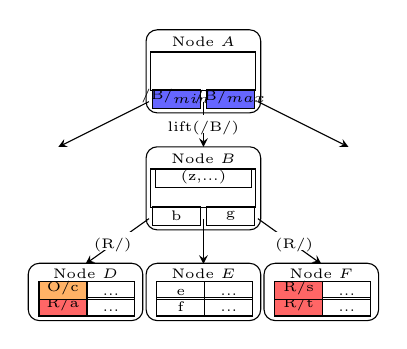
\begin{tikzpicture}[xscale=0.95, yscale=0.95]
            \node[anchor=south, rectangle, rounded corners, minimum height=.06\textwidth, minimum width=.12\textwidth, draw=black] at (.13\textwidth, 0) {};
            \node[anchor=south, font=\tiny] at (.13\textwidth, .036\textwidth) {Node $D$};
            \node[anchor=south, rectangle, minimum height=.015\textwidth, minimum width=.05\textwidth, draw=black, fill={red!60}] at (.105\textwidth, .005\textwidth) {};
            \node[anchor=south, font=\tiny] at (.105\textwidth, 0) {R/a};
            \node[anchor=south, rectangle, minimum height=.015\textwidth, minimum width=.05\textwidth, draw=black] at (.158\textwidth, .005\textwidth) {};
            \node[anchor=south, font=\tiny] at (.158\textwidth, 0) {...};
            \node[anchor=south, rectangle, minimum height=.015\textwidth, minimum width=.05\textwidth, draw=black, fill={orange!60}] at (.105\textwidth, .023\textwidth) {};
            \node[anchor=south, font=\tiny] at (.105\textwidth, .018\textwidth) {O/c};
            \node[anchor=south, rectangle, minimum height=.015\textwidth, minimum width=.05\textwidth, draw=black] at (.158\textwidth, .023\textwidth) {};
            \node[anchor=south, font=\tiny] at (.158\textwidth, .018\textwidth) {...};

            \node[anchor=south, rectangle, rounded corners, minimum height=.06\textwidth, minimum width=.12\textwidth, draw=black] at (.26\textwidth, 0) {};
            \node[anchor=south, font=\tiny] at (.26\textwidth, .036\textwidth) {Node $E$};
            \node[anchor=south, rectangle, minimum height=.015\textwidth, minimum width=.05\textwidth, draw=black] at (.235\textwidth, .005\textwidth) {};
            \node[anchor=south, font=\tiny] at (.235\textwidth, 0) {f};
            \node[anchor=south, rectangle, minimum height=.015\textwidth, minimum width=.05\textwidth, draw=black] at (.288\textwidth, .005\textwidth) {};
            \node[anchor=south, font=\tiny] at (.288\textwidth, 0) {...};
            \node[anchor=south, rectangle, minimum height=.015\textwidth, minimum width=.05\textwidth, draw=black] at (.235\textwidth, .023\textwidth) {};
            \node[anchor=south, font=\tiny] at (.235\textwidth, .018\textwidth) {e};
            \node[anchor=south, rectangle, minimum height=.015\textwidth, minimum width=.05\textwidth, draw=black] at (.288\textwidth, .023\textwidth) {};
            \node[anchor=south, font=\tiny] at (.288\textwidth, .018\textwidth) {...};

            \node[anchor=south, rectangle, rounded corners, minimum height=.06\textwidth, minimum width=.12\textwidth, draw=black] at (.39\textwidth, 0) {};
            \node[anchor=south, font=\tiny] at (.39\textwidth, .036\textwidth) {Node $F$};
            \node[anchor=south, rectangle, minimum height=.015\textwidth, minimum width=.05\textwidth, draw=black, fill={red!60}] at (.365\textwidth, .005\textwidth) {};
            \node[anchor=south, font=\tiny] at (.365\textwidth, 0) {R/t};
            \node[anchor=south, rectangle, minimum height=.015\textwidth, minimum width=.05\textwidth, draw=black] at (.418\textwidth, .005\textwidth) {};
            \node[anchor=south, font=\tiny] at (.418\textwidth, 0) {...};
            \node[anchor=south, rectangle, minimum height=.015\textwidth, minimum width=.05\textwidth, draw=black, fill={red!60}] at (.365\textwidth, .023\textwidth) {};
            \node[anchor=south, font=\tiny] at (.365\textwidth, .018\textwidth) {R/s};
            \node[anchor=south, rectangle, minimum height=.015\textwidth, minimum width=.05\textwidth, draw=black] at (.418\textwidth, .023\textwidth) {};
            \node[anchor=south, font=\tiny] at (.418\textwidth, .018\textwidth) {...};

            \node[anchor=south, rectangle, rounded corners, minimum height=.087\textwidth, minimum width=.12\textwidth, draw=black] at (.26\textwidth, .1\textwidth) {};
            \node[anchor=south, font=\tiny] at (.26\textwidth, .163\textwidth) {Node $B$};
            \node[anchor=south, rectangle, minimum height=.015\textwidth, minimum width=.05\textwidth, draw=black] at (.23\textwidth, .105\textwidth) {};
            \node[anchor=south, font=\tiny] at (.23\textwidth, .1\textwidth) {b};
            \node[anchor=south, rectangle, minimum height=.015\textwidth, minimum width=.05\textwidth, draw=black] at (.29\textwidth, .105\textwidth) {};
            \node[anchor=south, font=\tiny] at (.29\textwidth, .1\textwidth) {g};
            \node[anchor=south, rectangle, minimum height=.04\textwidth, minimum width=.11\textwidth, draw=black] at (.26\textwidth, .125\textwidth) {};
            \node[anchor=south, rectangle, minimum height=.015\textwidth, minimum width=.1\textwidth, draw=black] at (.26\textwidth, .147\textwidth) {};
            \node[anchor=south, font=\tiny] at  (.26\textwidth, .141\textwidth) {\putm(z,...)};

            \node[anchor=south, rectangle, rounded corners, minimum height=.087\textwidth, minimum width=.12\textwidth, draw=black] at (.26\textwidth, .229\textwidth) {};
            \node[anchor=south, font=\tiny] at (.26\textwidth, .292\textwidth) {Node $A$};
            \node[anchor=south, rectangle, minimum height=.015\textwidth, minimum width=.05\textwidth, draw=black, fill={blue!60}] at (.23\textwidth, .234\textwidth) {};
            \node[anchor=south, font=\tiny] at (.23\textwidth, .229\textwidth) {/B/$_{min}$};
            \node[anchor=south, rectangle, minimum height=.015\textwidth, minimum width=.05\textwidth, draw=black, fill={blue!60}] at (.29\textwidth, .234\textwidth) {};
            \node[anchor=south, font=\tiny] at (.29\textwidth, .229\textwidth) {/B/$_{max}$};
            \node[anchor=south, rectangle, minimum height=.04\textwidth, minimum width=.11\textwidth, draw=black] at (.26\textwidth, .254\textwidth) {};

            \draw[->, >=stealth] (.20\textwidth, .113\textwidth) -- (.13\textwidth, .063\textwidth);
            \draw[->, >=stealth] (.26\textwidth, .113\textwidth) -- (.26\textwidth, .063\textwidth);
            \draw[->, >=stealth] (.32\textwidth, .113\textwidth) -- (.39\textwidth, .063\textwidth);
            \draw[->, >=stealth] (.26\textwidth, .242\textwidth) -- (.26\textwidth, .192\textwidth);
            \draw[->, >=stealth] (.20\textwidth, .242\textwidth) -- (.10\textwidth, .192\textwidth);
            \draw[->, >=stealth] (.32\textwidth, .242\textwidth) -- (.42\textwidth, .192\textwidth);

            \node[anchor=north,rectangle, minimum height=.015\textwidth, minimum width=.05\textwidth, fill={white}] at (.16\textwidth, .099\textwidth) {};
            \node[anchor=north, font=\tiny] at (.16\textwidth, .102\textwidth) {\xf (R/)};
            \node[anchor=north,rectangle, minimum height=.015\textwidth, minimum width=.05\textwidth, fill={white}] at (.36\textwidth, .099\textwidth) {};
            \node[anchor=north, font=\tiny] at (.36\textwidth, .102\textwidth) {\xf (R/)};
            \node[anchor=north,rectangle, minimum height=.015\textwidth, minimum width=.08\textwidth, fill={white}] at (.26\textwidth, .228\textwidth) {};
            \node[anchor=north, font=\tiny] at (.26\textwidth, .231\textwidth) {lift(/B/)};
        \end{tikzpicture}
        \caption{\label{subfig:xf-2} To remove the \xf function, it discards
            exterior children and adds \xf functions to parent-to-child pointers
            of fringe children.}
    \end{subfigure}
    \caption[Resolving \xf functions in node flushes]{\label{fig:xf}
        During node flushes, the lifted \bedag resolves the \xf
        function associated with the parent-to-child pointer.}
\end{figure}

Figure~\ref{fig:xf} shows an example of fixing \xf functions in node flushes.
In Figure~\ref{subfig:xf-1}, the parent-to-child pointer from Node $A$ to
Node $B$ has an \xf function, \xf(``/R/'').
The key range specified by Node $A$ is (``/B/$_{min}$'',``/B/$_{max}$''),
and the \xf function translates the key range to
translates to (``/R/$_{min}$'',``/R/$_{max}$'') in Node $B$.
Also, the \xf function tells queries to ignore pivots and messages that are
out of the key range (``/R/$_{min}$'',``/R/$_{max}$'').
In Figure~\ref{subfig:xf-2}, the lifted \bedag garbage collects exterior nodes,
Node $C$ and $G$
and adds \xf functions to pointers to fringe nodes, Node $D$ and $F$.
Also, it updates keys in Node $B$ by removing the prefix, ``/R/'',
in the \xf function.
Note, the message \putm(/G/a,...) is also removed from Node $B$
because it is out of the key range specified in Node $A$.

\section{Implementation}
\label{sec:rc:impl}

This section discusses implementation details of the range-clone operation.

\subsection{Synchronization}

The range-clone operation synchronizes with other \bet operations using the
readers-writer locks of \bet nodes
(Section~\ref{sec:bg:impl:sync}).
The range-clone operation first grabs the write lock of the root node.
Then, while flushing messages along the root-to-leaf path until the LCA,
the range-clone operation write-locks \bet nodes, hand-over-hand,
holding the write lock of the root node.
Finally, the range-clone operation injects the \goto message into the root node
and releases the write locks of the root node and the LCA.

Compared to the range-rename operation that unlocks the root node after flushing
messages (Section~\ref{sec:rr:impl:sync}),
the range-clone operations locks the root node for a longer time.
However, the range-clone operation returns to the caller earlier,
while the range-rename operation needs to lock the LCAs during bottom-up
slicing, preventing concurrent operations to the subtrees.

\subsection{Preferential splitting}
\label{sec:rc:impl:pfsplit}

Most of the work in range-clone and range-rename is about splitting fringe
nodes, separating keys with the prefix and keys without the prefix.
If all nodes are either interior nodes or exterior nodes, much less work is
needed.
Therefore, it is beneficial to reduce the number of fringe nodes.

To this end, we introduce preferential splitting in node splits.
Originally, \fti splits leaf nodes evenly.
When a leaf node needs to be split, the middle key in the leaf is picked as the
new pivot that separates the two new leaf nodes.

Preferential splitting generates pivots that are potential splitting keys in
file system renames and maximizes the common prefix under the leaf,
subject to the constraint that both leaves should be at least 1/4 full.
This strategy reduces the likelihood of having fringe nodes
in range-clone and bounds how unbalanced leaves can be.

A naive approach would compare all keys in the range of [1/4, 3/4] of the leaf
node and pick the pair of two adjacent keys that share the shortest common
prefix.
But this scan can be costly.
For example, in \betrfs, a full leaf node is 4 MiB in size and each key/value pair in
\texttt{meta\_db} is less than 200 Bytes, which means more than 10000 key
comparisons are required in this naive preferential splitting.

In fact, we can do preferential splitting that only requires the reading of two keys.
Because the shortest common prefix of adjacent keys is the same as the common
prefix of the smallest (at 1/4 of the leaf) candidate key, $k_{s}$, and
the largest (at 3/4 of the leaf) candidate key, $k_{l}$,
a good pivot can be constructed from these two keys.
In particular, preferential splitting generates a pivot that is the maximum key
with prefix $p_{s}$, where $p_{s}$ is the shortest prefix of $k_{s}$ that
contains the LCP of $k_{s}$ and $k_{l}$ and has a slash or a end-of-string as
the last character.
For instance, if $k_{s}$ is ``/foo/bar'' and $k_{l}$ is ``/fuz/bar'',
preferential splitting set $p_{s}$ as ``/foo/'', which is the shortest prefix
of $k_{s}$ that contains the LCP of $k_{s}$ and $k_{l}$, ``/f'', and has a
slash at the end.
Therefore, the pivot generated by preferential splitting is the maximum key with
prefix ``/foo/'' (adding a `\textbackslash xff').

Non-leaf-node splits can be viewed as promoting a pivot from the child to the
parent.
Because the number of pivots in a non-leaf node is small (at most 16), we can
afford one-to-one comparisons.

As we will see in the evaluation, preferential splitting also helps
other operations, such as sequential writes, because the \bet is more likely
to generate a pivot that is the maximum data key of a file or directory.
In the sequential write workload, all pivots generated by node splits are
data keys of the file being written.
Generating the maximum data key of the file at the beginning of the workload
reduces node re-lifting costs.

\subsection{Queries}

As described in Section~\ref{sec:bg:impl:query}, during a query,
\fti applies messages in non-leaf nodes along the root-to-leaf path to the
leaf nodes.

However, in a \bedag,
there can be multiple paths from the root node to a leaf node,
which will accumulate a different set of pending messages.
Therefore, in our implementation,
we must cache different versions of the same node that is shared on disk --- one per path.
In addition to the original identifier, the node ID, in the cahe table,
we add the key range as a sub-identifier.
However, this approach can potentially create more cache pressure,
which can lead to more node evictions and I/Os.

We adopt a hybrid approach in the implementation.
If a leaf has only one version, i.e., all nodes along any path to it have
reference count 1, messages are applied to the leaf directly.
Otherwise, the leaf node maintains one additional copy for each version.

\subsection{Garbage collection}

When a leaf node's reference count drops to zero,
it is simply marked as free in the block table,
and the space on disk can be re-allocated after the next checkpoint.
If the system crashes before the next checkpoint, crash recovery will replay the
redo log on the previous checkpoint.
Therefore, it is only safe to reuse space in the block table
after a checkpoint (which includes a snapshot of the block table)
and we defer re-allocation of physical space until after a checkpoint
When an interior node's reference count drops to zero, the complication
is that, as part of freeing the node, the reference count on each of its children
must be lowered, and the children recursively freed.

Our \bedag implementation does this work with background threads,
although, in future work, we could also trigger foreground garbage collection
as part of flushing if free space falls below a threshold.
We track the pending work with an in-memory work queue and an extra flag in the block table;
the flag in the block table ensures that checkpointing the system is not obstructed by garbage collection,
and ensures that pending garbage collection work and space is not lost upon a crash.

\section{Conclusion}

This chapter presents the new range-clone operation.
We first describe a range-clone implementation that finishes all works
on the critical path and transforms lifted \bets into lifted \bedags.
Then, we introduce the \goto message that delays tree surgery,
fitting the implementation into the write-optimized framework of lifted \bedags.
At last, we show how \goto messages should be flushed down the lifted \bedags.
A \goto message will eventually become pivots and a parent-to-child pointer
in the lifted \bedag.

Full-path-indexed \betrfs clones a directory without traversing the directory
because full-path indexing specifies the key range inside the directory.
In contrast, to finish a directory clone,
an inode-based file system needs to traverse the directory to collect all inodes
inside the directory.
When the number of inodes in the directory is large,
cloning the directory is slower in inode-based file systems
than that in full-path-indexed \betrfs.
Additionally, the directory clones in full-path-indexed \betrfs
still maintains full-path indexing, which ensures good locality.

Therefore, full-path indexing is not an obstacle to namespace operations.
In fact, full-path indexing creates more opportunities for namespace operations.

Similar to the range-rename operation, the technique is not limited to the
range-clone operation that clones keys with certain prefix.
For a key/value store operation that clones a lot of keys,
one can use a similar technique as long as the key/value store can group all
related keys in a contiguous key range and
there is an \xf function that translates sources keys to destination keys.

